%\documentclass[10pt,a4paper]{article}
\documentclass[10pt]{article}
%\usepackage[top=0.85in,left=2.75in,footskip=0.75in]{geometry}
\usepackage[english]{babel}
\usepackage[utf8x]{inputenc}
\usepackage[T1]{fontenc}
%\usepackage[a4paper]{geometry}
%\geometry{a4paper, top=1in, bottom=2in}
\usepackage{amsmath}
\usepackage{amssymb}
\usepackage{graphicx}
\usepackage[colorlinks=true, allcolors=blue, hypertexnames=false]{hyperref}
\usepackage{epsfig,amsfonts}
%\usepackage{natbib}
\usepackage{authblk}
%\usepackage{subfig}
\usepackage{subfigure} %w/ Lorin's edits
\usepackage{setspace}
\usepackage{hypcap}
\usepackage{lscape}
\usepackage{lineno} %can do [right] to shift location of #s
%From: https://www.overleaf.com/learn/how-to/Cross_referencing_with_the_xr_package_in_Overleaf
\usepackage{xr}
\makeatletter
\newcommand*{\addFileDependency}[1]{% argument=file name and extension
  \typeout{(#1)}
  \@addtofilelist{#1}
  \IfFileExists{#1}{}{\typeout{No file #1.}}
}
\makeatother
\newcommand*{\myexternaldocument}[1]{%
    \externaldocument{#1}%
    \addFileDependency{#1.tex}%
    \addFileDependency{#1.aux}%
}
\myexternaldocument{Main}
%From: https://tex.stackexchange.com/questions/64934/subfig-label-positioning (went with second example solution on how to get multiple figures aligned with subfig + desired labeling)
%\usepackage{floatrow}
%From: https://tex.stackexchange.com/questions/332295/command-textalpha-unavailable-in-encoding-t1-when-using-greek
\usepackage{textgreek}

%From Lorin
\usepackage{latexsym}
\usepackage{bm}
\usepackage{bbm}

\def\eq#1{(\ref{#1})}
\def\pdf{p.d.f.\ } \def\cdf{c.d.f.\ }
\def\pdfs{p.d.f.s} \def\cdfs{c.d.f.s}
\def\mgf{m.g.f.\ } \def\mgfs{m.g.f.s\ }
\def\ci{\perp   \perp}  % conditional independence symbol
\def\beginmat{ \left( \begin{array} }
\def\endmat{ \end{array} \right) }
\def\diag{{\rm diag}}
\def\log{{\rm log}}
\def\tr{{\rm tr}}
\def\cond{\, | \,}
\newcommand*\diff{\mathop{}\!\mathrm{d}}
%\newcolumntype{P}[1]{>{\centering\arraybackslash}p{#1}}

\newtheorem{claim}{Claim}[section]
\newtheorem{definition}{Definition}[section]
\newtheorem{thm}{Theorem}[section]
\newtheorem{prop}{Proposition}[section]

\def\dsum{\displaystyle\sum}
\def\dint{\displaystyle\int}
%\def\dfrac{\displaystyle\frac}
\def\dsup{\displaystyle\sup}
\def\dinf{\displaystyle\inf}
\def\dmin{\displaystyle\min}
\def\dlim{\displaystyle\lim}

\newcommand{\me}{\mathrm{e}}
\newcommand{\supp}{\operatorname{supp}}
\newcommand{\abs}[1]{\left|#1\right|}
\newcommand{\comment}[1]{{\em #1}}
\newcommand{\ba}{\mathbf{a}}
\newcommand{\bb}{\mathbf{b}}
\newcommand{\bc}{\mathbf{c}}
\newcommand{\be}{\mathbf{e}}
\newcommand{\bg}{\mathbf{g}}
\newcommand{\bl}{\mathbf{l}}
\newcommand{\bs}{\mathbf{s}}
\newcommand{\bq}{\mathbf{q}}
\newcommand{\bk}{\mathbf{k}}
\newcommand{\bv}{\mathbf{v}}
\newcommand{\bx}{\mathbf{x}}
\newcommand{\by}{\mathbf{y}}
\newcommand{\bz}{\mathbf{z}}
\newcommand{\bh}{\mathbf{h}}
\newcommand{\bu}{\mathbf{u}}
\newcommand{\bfm}{\mathbf{m}}
\newcommand{\bw}{\mathbf{w}}
\newcommand{\w}{\mathbf{w}}
\newcommand{\bp}{\mathbf{p}}
\newcommand{\bK}{\mathbf{K}}
\newcommand{\bV}{\mathbf{V}}
\newcommand{\bA}{\mathbf{A}}
\newcommand{\bB}{\mathbf{B}}
\newcommand{\bC}{\mathbf{C}}
\newcommand{\bX}{\mathbf{X}}
\newcommand{\bY}{\mathbf{Y}}
\newcommand{\bE}{\mathbf{E}}
\newcommand{\bG}{\mathbf{G}}
\newcommand{\bH}{\mathbf{H}}
\newcommand{\bP}{\mathbf{P}}
\newcommand{\bQ}{\mathbf{Q}}
\newcommand{\bR}{\mathbf{R}}
\newcommand{\bW}{\mathbf{W}}
\newcommand{\bM}{\mathbf{M}}
\newcommand{\bU}{\mathbf{U}}
\newcommand{\bZ}{\mathbf{Z}}
\newcommand{\bD}{\mathbf{D}}
\newcommand{\bI}{\mathbf{I}}
\newcommand{\bS}{\mathbf{S}}
\newcommand{\T}{\intercal}
\newcommand{\wt}{\widetilde}
\newcommand{\wh}{\widehat}

\newcommand{\E}{\mathbb{E}}
\newcommand{\V}{\mathbb{V}}

\newcommand{\bbE}{\mathbb{E}}
\newcommand{\bbV}{\mathbb{V}}
\newcommand{\N}{\mathcal{N}}

\newcommand{\bepsilon}{\boldsymbol\epsilon}
\newcommand{\bvarepsilon}{\boldsymbol\varepsilon}
\newcommand{\bbeta}{\boldsymbol\beta}
\newcommand{\bsigma}{\boldsymbol\sigma}
\newcommand{\tbbeta}{{\tilde{\boldsymbol\beta}}}
\newcommand{\tbeta}{{\tilde{\beta}}}
\newcommand{\bgamma}{\boldsymbol\gamma}
\newcommand{\bdelta}{\boldsymbol\delta}
\newcommand{\btheta}{\boldsymbol\theta}
\newcommand{\bpsi}{\boldsymbol\psi}
\newcommand{\bphi}{\boldsymbol\phi}
\newcommand{\brho}{\boldsymbol\rho}
\newcommand{\balpha}{\boldsymbol\alpha}
\newcommand{\bmu}{\boldsymbol\mu}
\newcommand{\bomega}{\boldsymbol\omega}
\newcommand{\btau}{\boldsymbol\tau}
\newcommand{\bDelta}{\boldsymbol\Delta}
\newcommand{\bOmega}{\boldsymbol\Omega}
\newcommand{\bSigma}{\boldsymbol\Sigma}
\newcommand{\bLambda}{\boldsymbol\Lambda}
\newcommand{\bTheta}{\boldsymbol\Theta}
\newcommand{\at}[2][]{#1|_{#2}}
\newcommand{\red}[1]{\textcolor{red}{#1}}
\newcommand{\blue}[1]{\textcolor{blue}{#1}}

%2020091 Additions from Lorin's main edits
\topmargin 0.0cm
\oddsidemargin 0.5cm
\evensidemargin 0.5cm
\textwidth 16cm 
\textheight 21cm

\usepackage{latexsym,color,multirow,soul,xspace,tabularx}
\usepackage{booktabs}
\usepackage{multirow,multicol}
\usepackage{grffile}
\usepackage{epstopdf}
\usepackage{longtable}
\usepackage{adjustbox} 
\usepackage{makecell}
\usepackage{sidecap}
\usepackage{algorithm}
\usepackage{algpseudocode}
\usepackage{tikz}
\usepackage{caption}
\usepackage[subfigure]{tocloft}
\usepackage{etoolbox}
\usepackage{pdflscape}
\pagestyle{myheadings}

\newcommand{\edit}[2]{\sout{#1}\textcolor{red}{\xspace#2}}
%\newcommand{\sr}[2]{\sout{#1}\textcolor{red}{#2}}
\newcommand{\black}{\textcolor{black}}
\newcommand{\genee}{gene-$\varepsilon$~}
\newcommand{\genE}{gene-$\varepsilon$}

\DeclareMathOperator*{\argmin}{arg\,min}
\DeclareMathOperator*{\argmax}{arg\,max}

\newcolumntype{R}[2]{%
    >{\adjustbox{angle=#1,lap=\width-(#2)}\bgroup}%
    l%
    <{\egroup}%
}
\newcommand*\rot{\multicolumn{1}{R{90}{1em}}}
\newcolumntype{P}[1]{>{\centering\arraybackslash}p{#1}}

% Bold the 'Figure #' in the caption and separate it with a period
% Captions will be left justified
\usepackage[labelfont=bf,labelsep=period,justification=justified]{caption}
\captionsetup[table]{name=Supplementary Table}
\captionsetup[figure]{name=Supplementary Figure}
\allowdisplaybreaks
\renewcommand\thesubfigure{(\alph{subfigure})}
\bibliographystyle{plos2015}
\usepackage{cite}

% Remove brackets from numbering in List of References
\makeatletter
\renewcommand{\@biblabel}[1]{\quad#1.}
\makeatother


%%%%%%%%%%%%
%%%%%%%%%%%%

%\title{Supplementary: Differential complex trait architecture across humans: epistasis identified in non-European populations at multiple genomic scales}
%\author[1,2]{Michael C. Turchin}
%\author[1,3]{Isabella Ting}
%\author[1,4,5,*]{Lorin Crawford}
%\author[1,2,*,$\dag$]{Sohini Ramachandran}
%\affil[1]{Center for Computational Molecular Biology, Brown University}
%\affil[2]{Department of Ecology and Evolutionary Biology, Brown University}
%\affil[3]{Department of Computer Science, Brown University}
%\affil[4]{Department of Biostatistics, Brown University}
%\affil[5]{Center for Statistical Science, Brown University}
%\affil[$\ast$]{indicates these authors contributed equally}
%\affil[$^\dag$]{To whom correspondence should be addressed: sramachandran@brown.edu}

\begin{document}
%\maketitle

% Title must be 150 characters or less
\begin{flushleft}
{\Large{\textbf{Supplementary Note to ``Pathway Analysis within Multiple Human Ancestries Reveals Novel Signals for Epistasis in Complex Traits''}}}
\newline
% Insert Author names, affiliations and corresponding author email.
\\
Michael C. Turchin\textsuperscript{1,2,$\dagger$}, Gregory Darnell\textsuperscript{2,3}, Lorin Crawford\textsuperscript{2,4,*,$\dagger$}, and Sohini Ramachandran\textsuperscript{1,2,*,$\dagger$} 
\\
\bigskip
\bf{1} Department of Ecology and Evolutionary Biology, Brown University, Providence, RI, USA
\\
\bf{2} Center for Computational Molecular Biology, Brown University, Providence, RI, USA
\\
\bf{3} Institute for Computational and Experimental Research in Mathematics (ICERM), Brown University, Providence, RI, USA
\\
\bf{4} Microsoft Research New England, Cambridge, MA, USA
\\
\bigskip
*: Authors Contributed Equally\\
$\dagger$ Corresponding E-mail: michael\_turchin@brown.edu; lcrawford@microsoft.com; sramachandran@brown.edu 
\end{flushleft}

\setcounter{figure}{0}
\setcounter{table}{0}
\setcounter{equation}{0}
\makeatletter 

\tableofcontents

\clearpage
\newpage

%\section{Supplementary Note}\label{Supplementary-Note}

\section{Data Quality Control Procedures for UK Biobank}

The results presented in the main text made use of genotyped chip data released from the UK Biobank \cite{Sudlow2015}. Here, we focus on subgroups in the UK Biobank included individuals based on their self-identified ancestries: ``African'', ``British'', ``Caribbean'', ``Chinese'', ``Indian'', and ``Pakistani'', respectively. Quality control procedures for each of these subgroups in the data are as follows. First, we removed (\textit{i}) SNPs with minor allele frequency (MAF) less than 1\%, (\textit{ii}) SNPs with missingness greater than 5\%, and (\textit{iii}) SNPs not in Hardy-Weinberg Equilibrium (Fisher's exact test $P > 10^{-6}$). We also removed individuals by checking three sets of criteria. First, we removed individuals if they were a 3rd degree relative (or more) to someone else in the dataset --- specifically, the KING relatedness values provided with the UK Biobank data were used to identify related individuals, and one individual from every pair of 3rd degree or more relatives was removed. Second, individuals were also removed if they were tagged by any of the following three flags within the UK Biobank data: \texttt{het.missing.outliers}, \texttt{putative.sex.chromosome.aneuploidy}, and \texttt{excess.relatives}. Lastly, individuals were removed if they were determined to be outliers via principal component analysis (PCA) --- this was conducted by running \texttt{FlashPCA} (version 2.1) \cite{Abraham2017} in \texttt{R} on each population subgroup separately and identifying individuals that had any of their top six principal component (PC) values greater than seven standard deviations away from the mean. We refer to conducting PCA on each subgroup separately as ``local PCA'' to help distinguish from the alternative setup of conducting PCA on the entire dataset jointly, which would be referred to as ``global PCA''. 

After the first round of quality control procedures, we then proceeded to impute missing genotypes for each population subgroup. To conduct this imputation, we uploaded our population subgroups to the University of Michigan Imputation Server \cite{Das2016} and used the following options: \texttt{Minimac3} for the imputation software, 1000 Genomes (phase 3 version 5) for the reference panel, and \texttt{Eagle} (version 2.3) for the phasing software. Completed imputed files were then downloaded from the Imputation Server afterwards and treated to one last round of quality control. Here, imputed variants were intersected back to the original set of genotyped chip variants. Variants with imputation quality scores  less than 30\% were removed, and variants that had genotype missingness greater than 0\% were also removed. Information on the final forms of our UK Biobank population subgroups can be found in Supplementary Table \ref{InterPath-Supp-Table-UKBPopStats}.

\section{Hypergeometric Enrichment Analyses}

Hypergeometric analyses were conducted by counting the number of times a given gene is present among the significant pathways identified by MAPIT-R for a given database-phenotype-subgroup combination versus the number of times the gene is present among the background distribution of pathways from the same database. For the size-restriction analyses, pathways with greater than 1,000 SNPs were removed. The 1,000 SNP threshold was chosen to balance between the total number of pathways removed and the average pathway size across all subgroups (see Supplementary Figure \ref{InterPath-Supp-Figure-pValsVsNumSNPs} for the relationship between MAPIT-R $P$-values and pathway sizes). Note that for a number of size thresholds ranging from 500 to 1,500 SNPs, results regarding the proteasome family genes remain robust (Supplementary Figure \ref{InterPath-Supp-Figure-Hypergeoemtric-SizeThresholds}).

\clearpage

\section{Supplementary Figures}\label{Supplementary-Figures}

%\renewcommand{\thefigure}{Supplementary Figure \arabic{figure}}
%\renewcommand{\thetable}{Supplementary \arabic{table}}
\renewcommand{\figurename}{Supplementary Figure}
\renewcommand{\tablename}{Supplementary Table}
\setcounter{figure}{0}
\setcounter{table}{0}

\begin{figure}[H]
\centering
%\hspace*{-1cm}
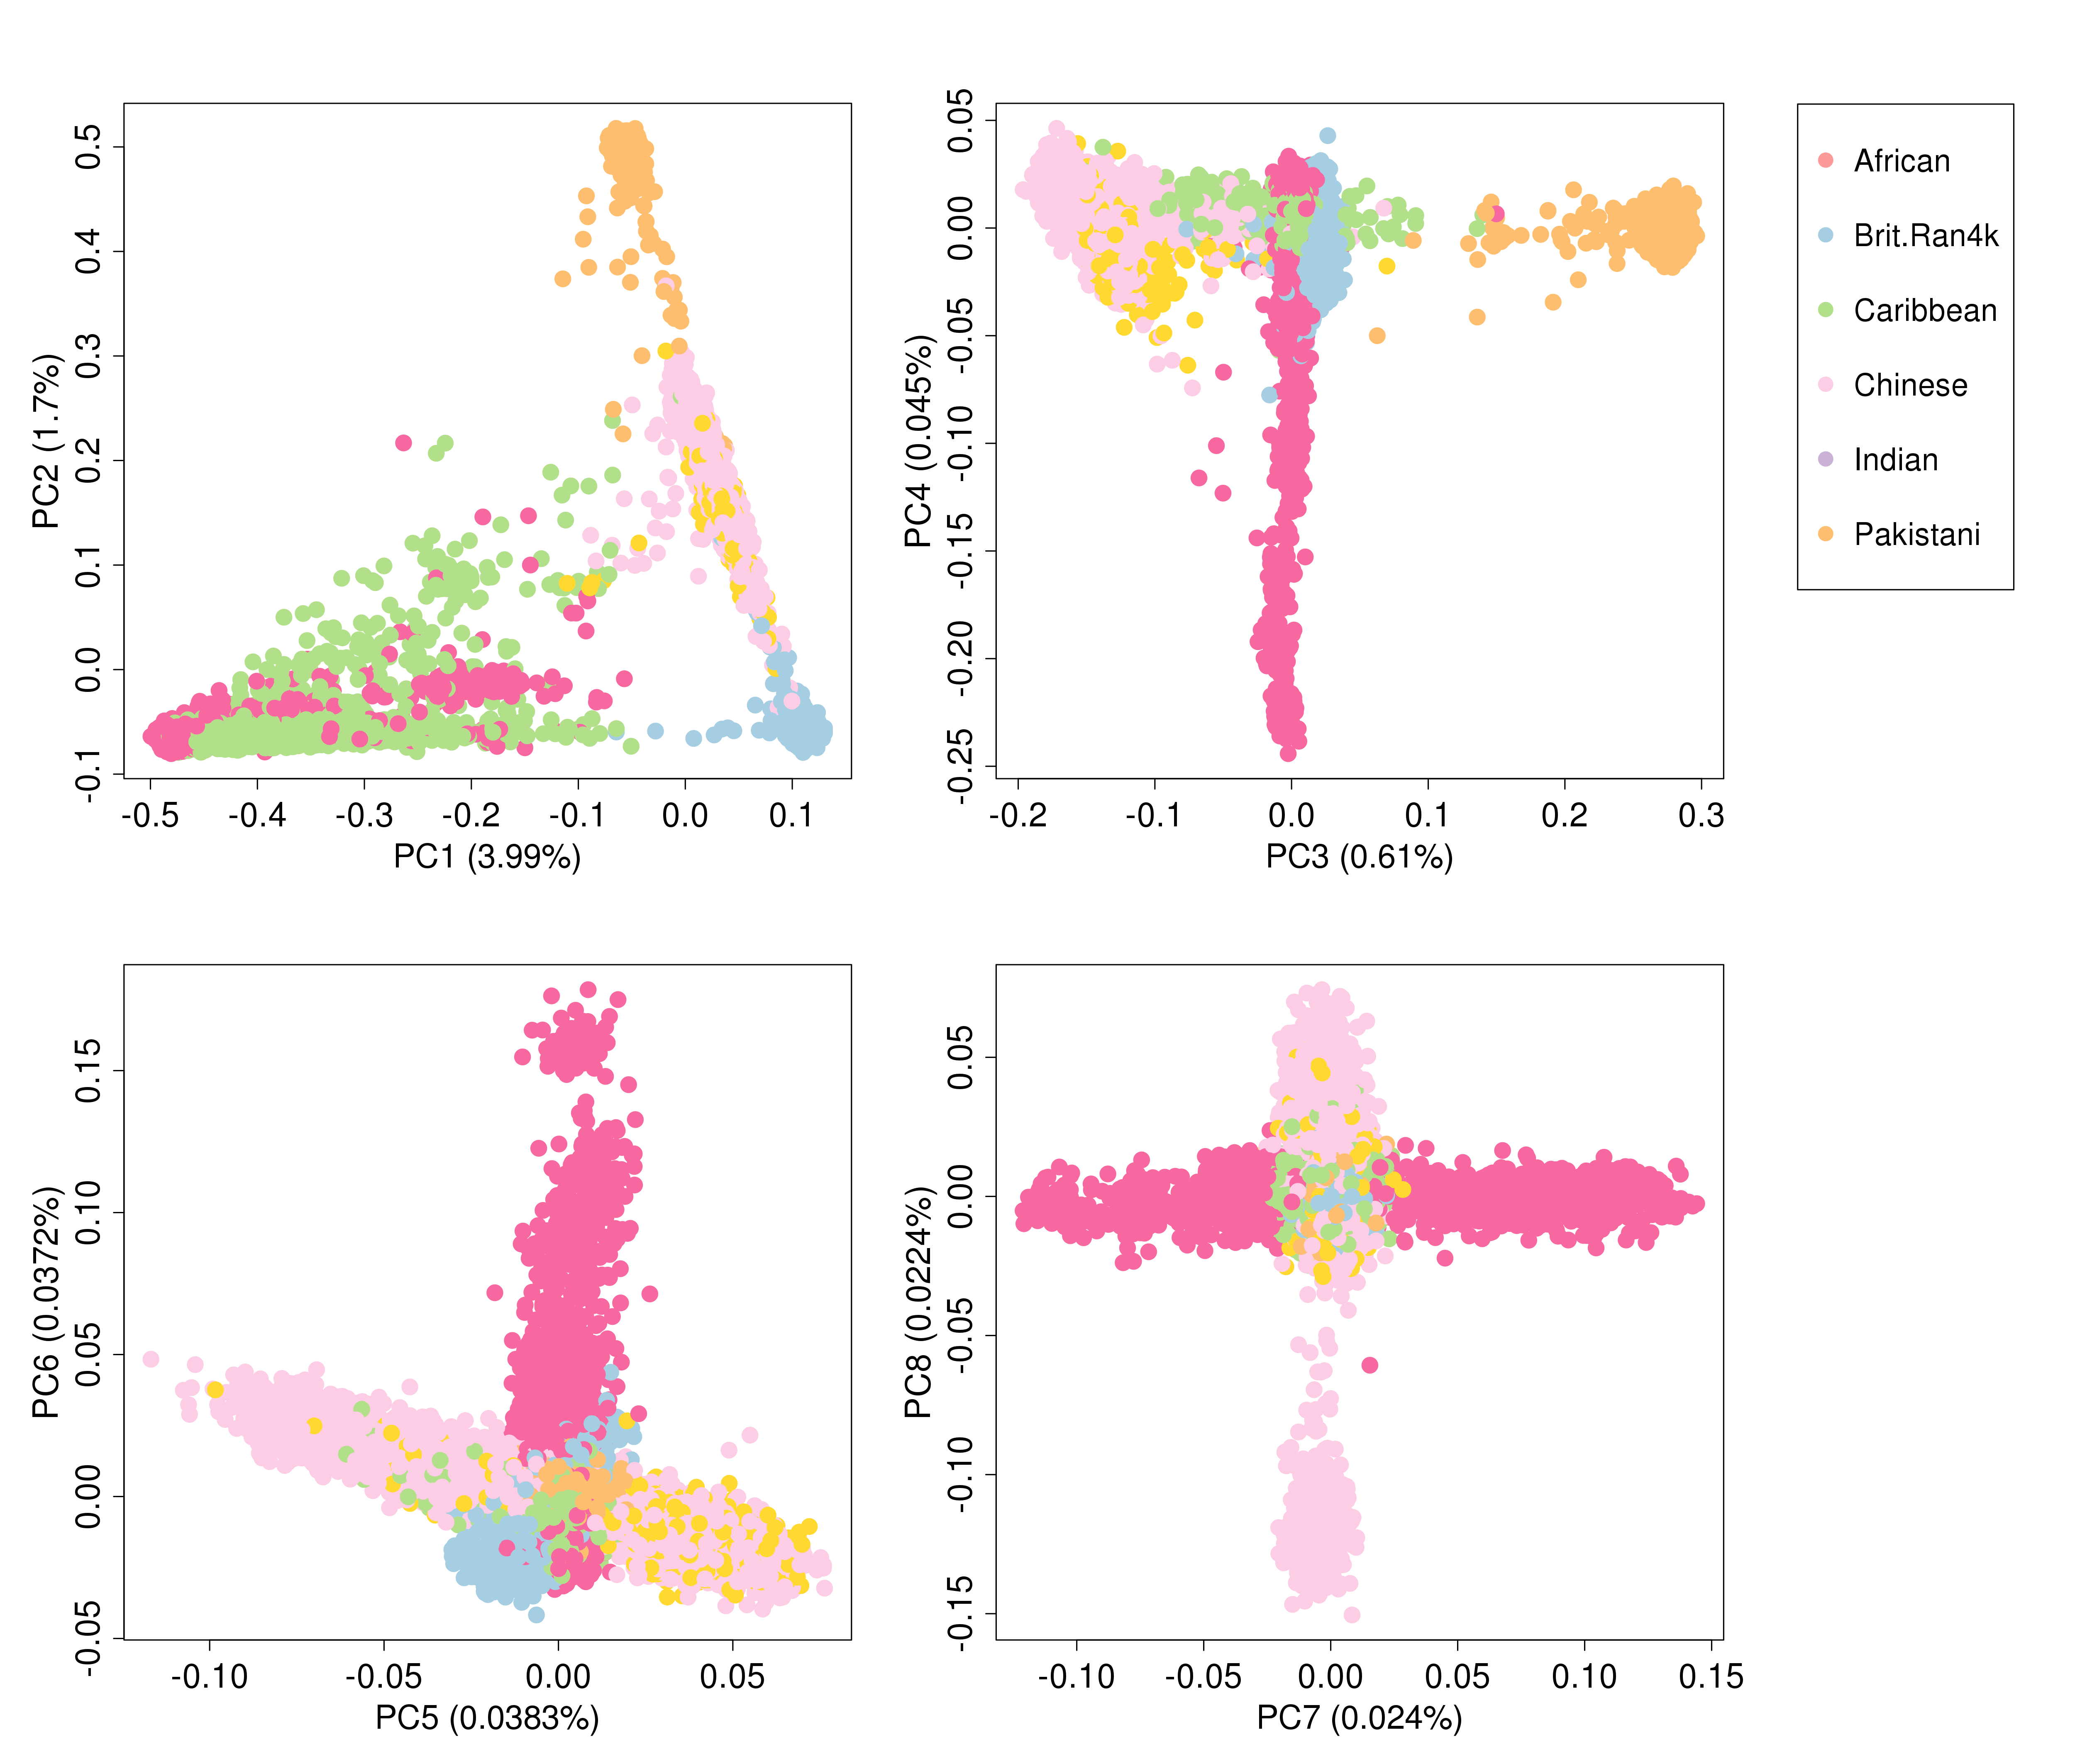
\includegraphics[width = \textwidth]{Images/Supp/InterPath_Supp_Figure_UKB_PCAPlot_vs2.png}
\caption{\textbf{Global principal component analysis (PCA) of the different ancestry-specific subgroups in the UK Biobank}. Here, subgroups in the UK Biobank included individuals based on their self-identified ancestries: ``African'', ``British'', ``Caribbean'', ``Chinese'', ``Indian'', and ``Pakistani'', respectively. The figure shows the top eight global principal components (PCs) for each subgroup plotted against one another. The comparisons include: \textbf{(a)} PC1 vs.~PC2, \textbf{(b)} PC3 vs.~PC4, \textbf{(c)} PC5 vs.~PC6, and \textbf{(d)} PC7 vs.~PC8. PCA was conducted using \texttt{FlashPCA} \cite{Abraham2017}. Here, ``global'' refers to running PCA on the full UK Biobank dataset with all subgroups pulled together jointly. This is in contrast to `local' PCA which conducts principal component analysis on each subgroup separately. Note that global PCs was only used for exploratory analyses and to create these plots, while local PCs were used for quality control and to adjust for population structure in the MAPIT-R analyses. On each axis, we also list the percent of total variation explained (PVE) by each PC in parentheses.}
\label{InterPath-Supp-Figure-UKB-subgroups-PCAPlot}
\end{figure}
\clearpage

\begin{figure}[htbp]
\centering
%\hspace*{-.9cm}
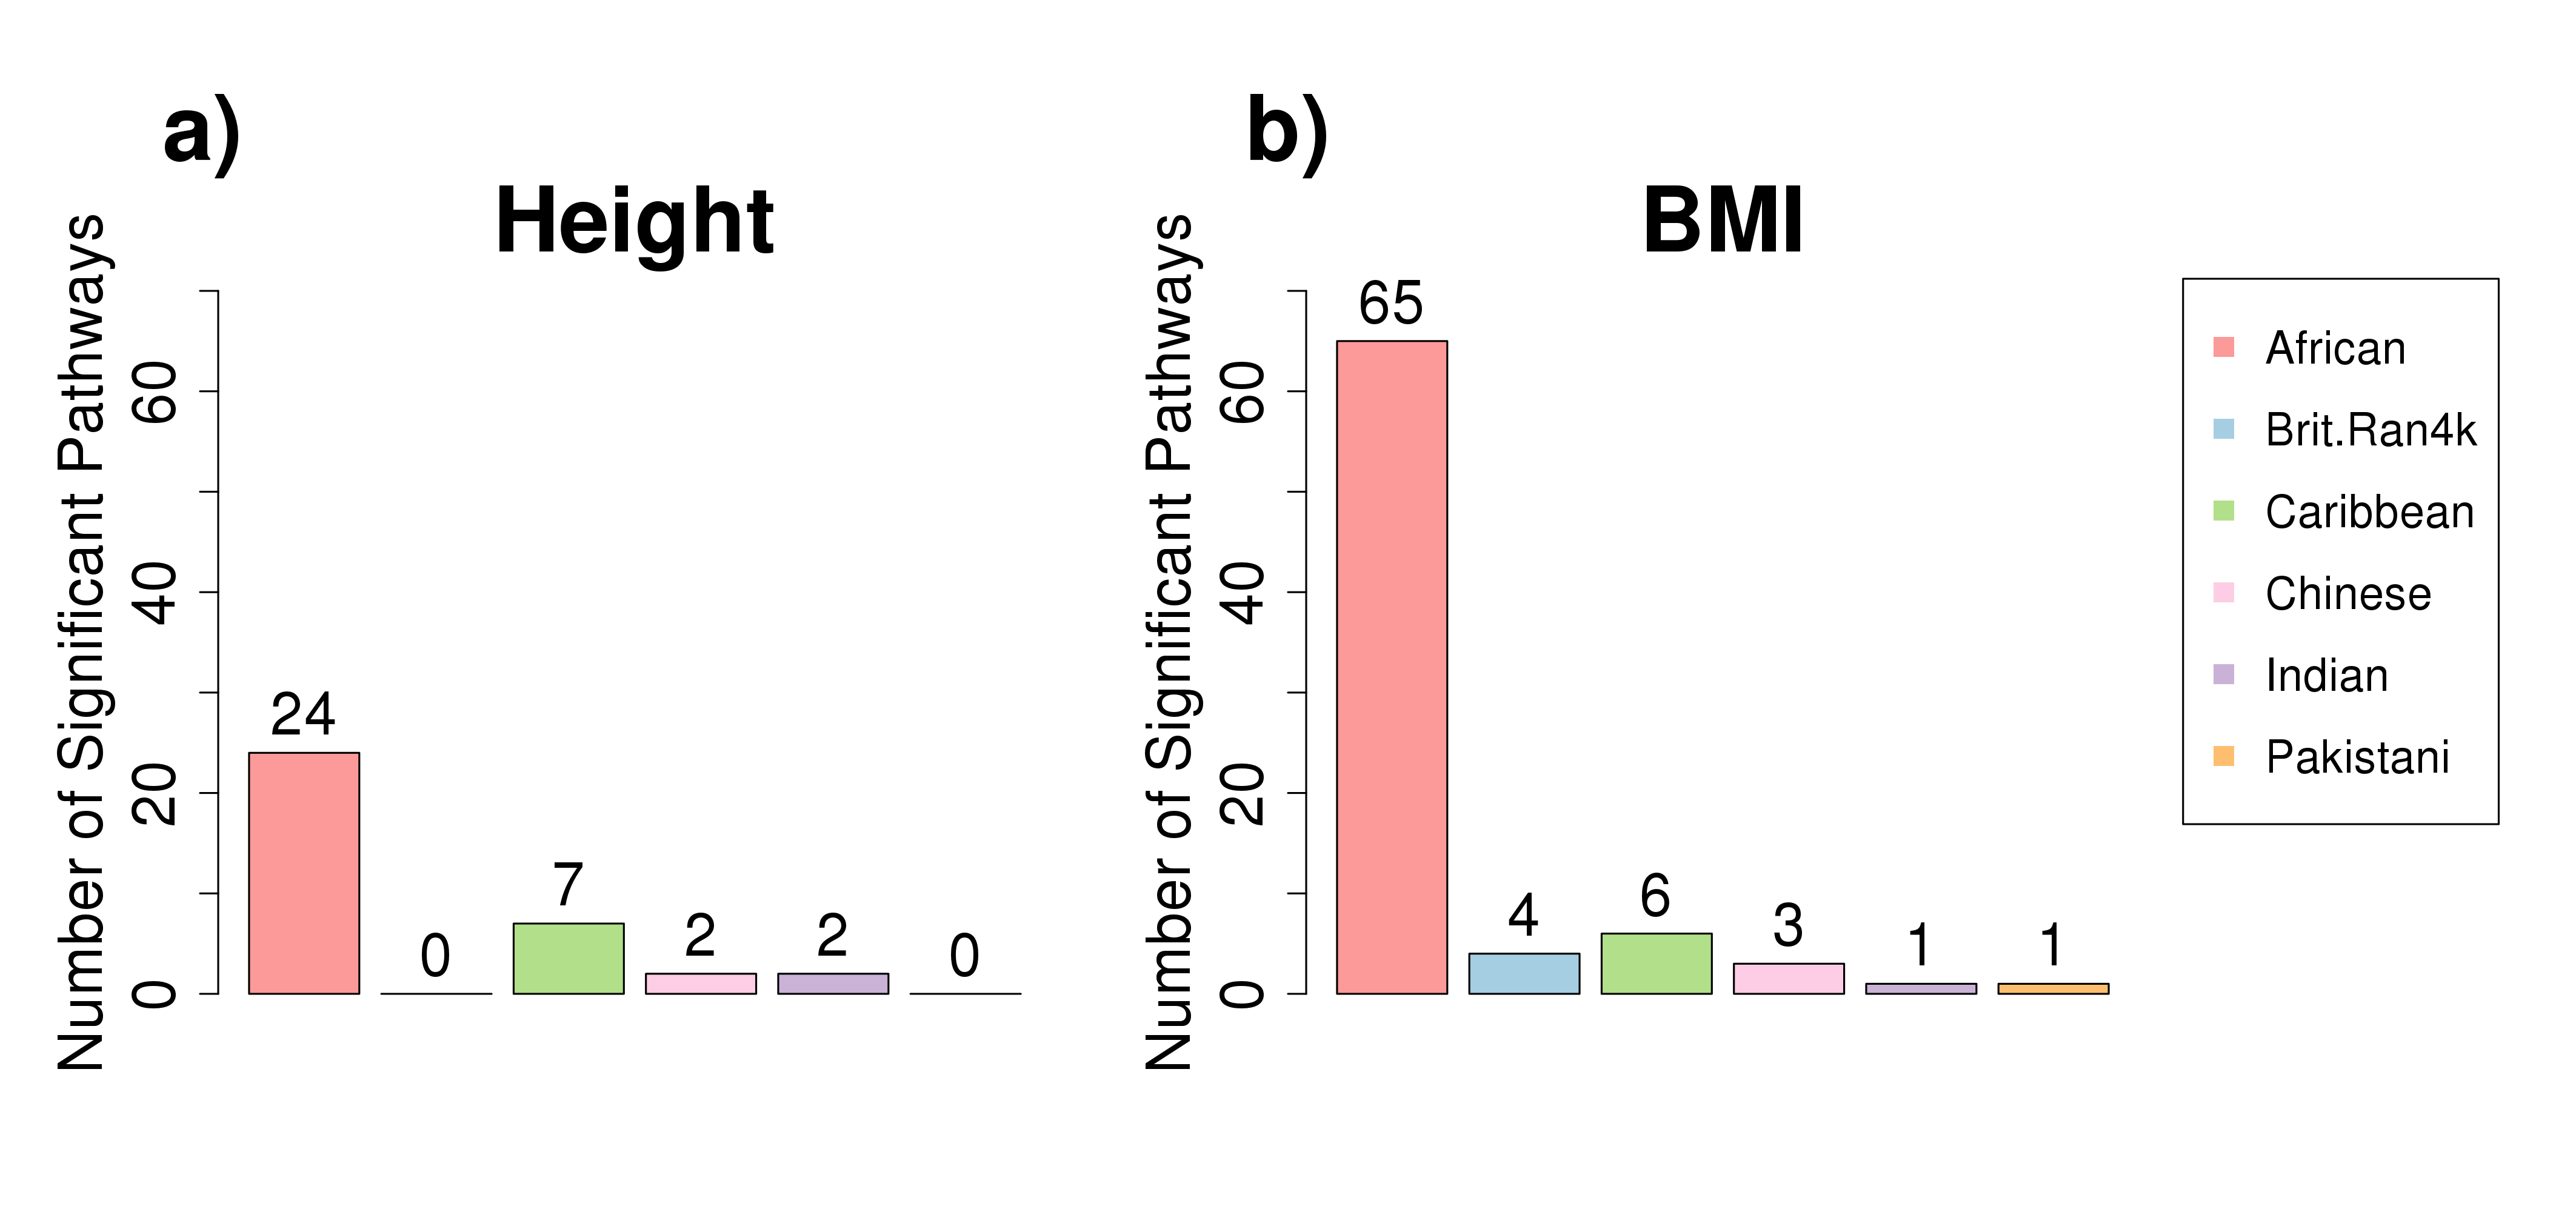
\includegraphics[width = \textwidth]{Images/Supp/InterPath_Supp_Figure_Barplots_REACTOME_vs4.png}
\caption{\textbf{Number of REACTOME pathways identified by MAPIT-R that have significant marginal epistatic effects within (a) standing height and (b) body mass index (BMI) per subgroup in the UK Biobank.} Here, the subgroups in the UK Biobank included individuals based on their self-identified ancestries: ``African'', ``British'', ``Caribbean'', ``Chinese'', ``Indian'', and ``Pakistani'', respectively. Genome-wide significance was determined by using Bonferroni-corrected $P$-value thresholds based on the number of pathways tested in each database-phenotype-subgroup combination (see Supplementary Table \ref{InterPath-Supp-Table-UKBPopStats}). Across all database-phenotype combinations, the African subgroup has the largest numbers of significant pathways. For lists of the specific significant pathways per database-phenotype-subgroup combination, see Supplementary Table \ref{InterPath-Supp-Table-TopPathways-AllPaths-AllPhenos}.}
\label{InterPath-Supp-Figure-Barplots-REACTOME}
\end{figure}
\clearpage

\begin{figure}[htbp]
\centering
\subfigure[Num1]{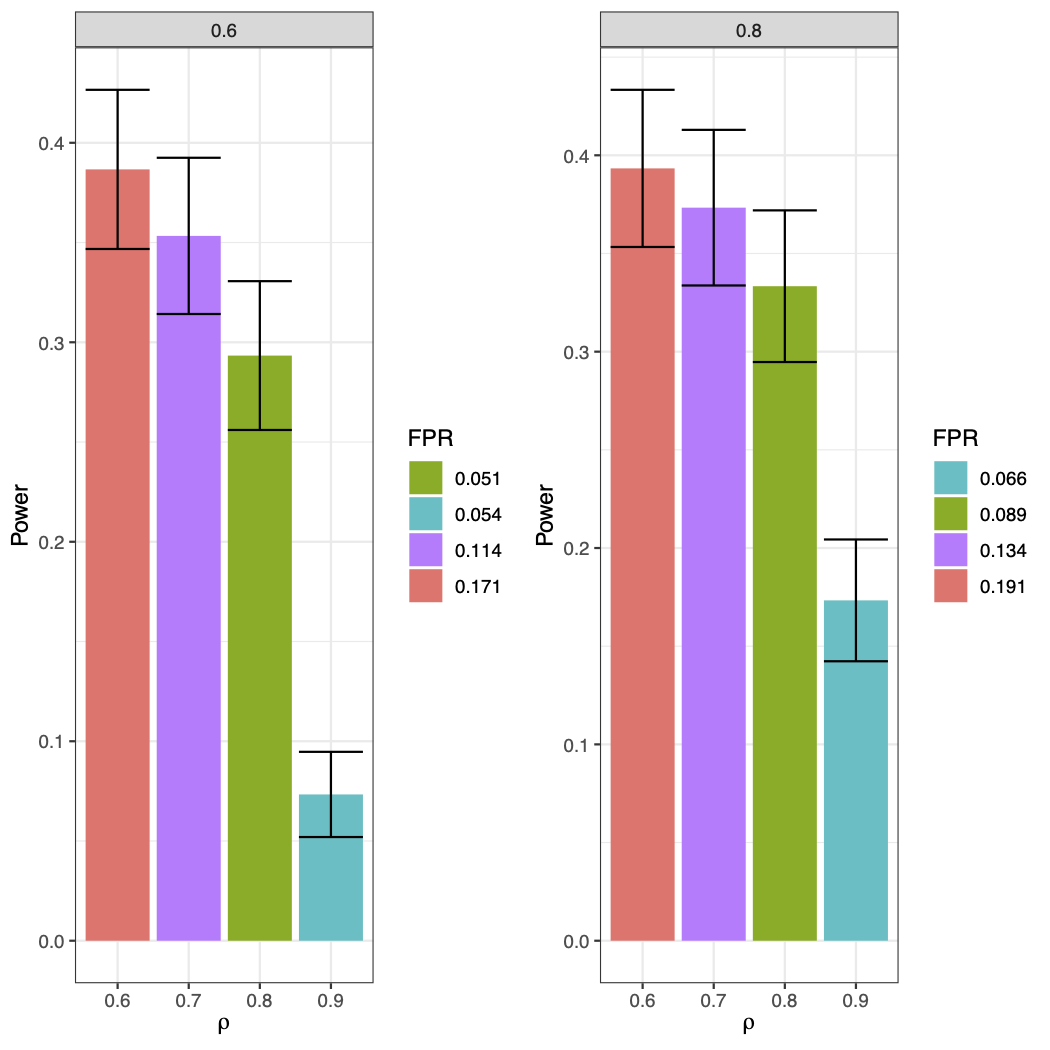
\includegraphics[width=.4\textwidth]{Images/Supp/Greg/power_split.png}}
\subfigure[Num2]{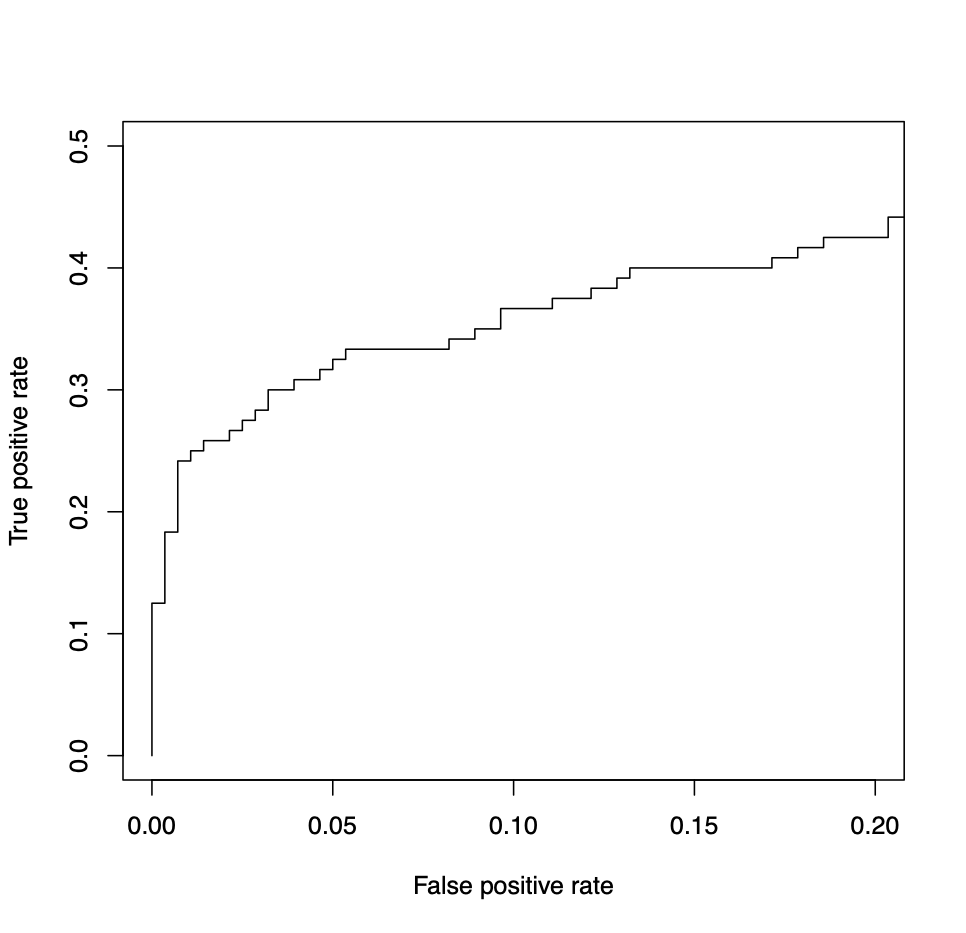
\includegraphics[width=.4\textwidth]{Images/Supp/Greg/Rplot01.png}}
\subfigure[Num3]{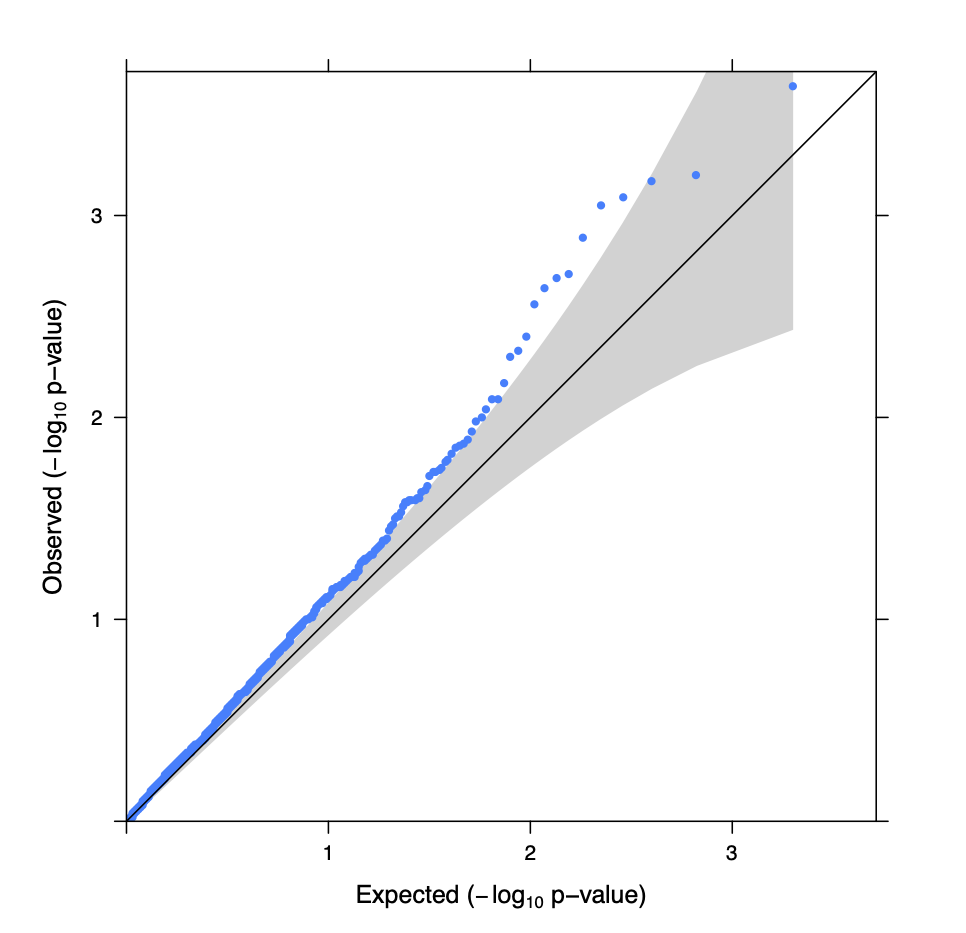
\includegraphics[width=.4\textwidth]{Images/Supp/Greg/Rplot02.png}}
\subfigure[Num4]{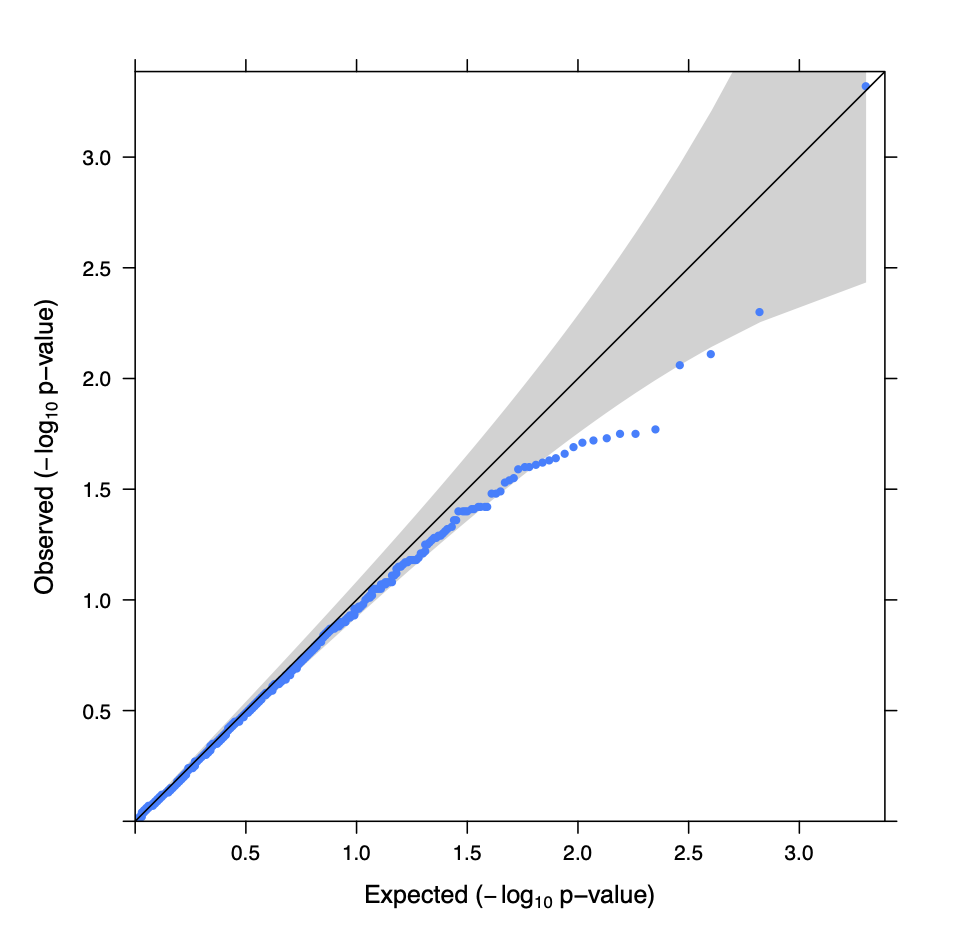
\includegraphics[width=.4\textwidth]{Images/Supp/Greg/Rplot03.png}}
\caption{\textbf{Plots showing behavior of MAPIT-R under simulations of varying genetic architectures and pathway definitions}. Here, we run simulations of MAPIT-R under various biological scenarios. For all plots, 3,000 individuals from the British subgroup and 10,000 SNPs from chromosome 1 were used to simulate different phenotypes based on varying additive and non-additive genetic architectures. Each simulation contains 10 pathways, each of which contains 50 SNPs. For each pathway, every SNP is `interacting', meaning each SNP of the 50 has 200 `interacting SNPs' randomly chosen elsewhere among the remaining 9,950 background SNPs. To properly simulate background additive heritability, an additional 50\% of the background, non-interacting SNPs were assigned additive effects. Overall heritability ($H^2$) was set at .6 or .8. Additive heritability was set at $H^2*(\rho)$ and epistatic heritability was set at $H^2*(1-\rho)$, where $\rho$ is a value ranging from .9 to .6 that controls the ratio between. Lastly, the top 10 local principal components of the individuals were used to introduce population structure and account for 10\% of the overall phenotype variance. (a) additive to epistatic heritability.  Each pathway has
%For all plots, number of individuals = 3,000. Number of SNPs total = 10,000. Genotypes are from uk biobank, chromosome 1. First 10k SNPs and random 3k white british individuals. There are 10 pathways in each simulation. Each pathway has exactly 50 group 1 SNPs and 200 interactions per group 1 SNP, so 10,000 total group 2 SNPs. Group 3 SNPs, which is those SNPs that have an additive background is 50\% of the total SNPs chosen at random, so 5,000 SNPs. Overall heritability is (0.6 or 0.8 for power plots) $H^2$. Epistatic PVE is $H^2*(1-\rho)$. And additive heritability is $H^2*(\rho)$. 10 global population structure PCs are included in each simulation and account for 10\% of the overall phenotype variance.
%A) power plot: $H^2$ on the top facet. $\rho$ on the x-axis. power = true positive rate on the y-axis. false positive rate is color. 50 simulations are performed per rho/pve combo. error bars are standard errors across 50 simulations.
%B) ROC curve: true positive rate vs false positive rate across 100 simulations with 10 pathways per sim. 5 are true positives and 5 are true negatives. I need to double check these stats for the ROC curve.
%C) QQ\_overlap: and D) QQ\_disjoint: 50 simulations. 10 pathways in each. same as the power plots. overlap vs disjoint refers to whether the SNPs in *group 1* so the main pathway SNPs could contain any duplicates across pathways tested in the same simulation.}
}
\label{InterPath-Supp-Figure-Greg-Simulations}
\end{figure}
\clearpage

\begin{figure}[htbp]
\centering
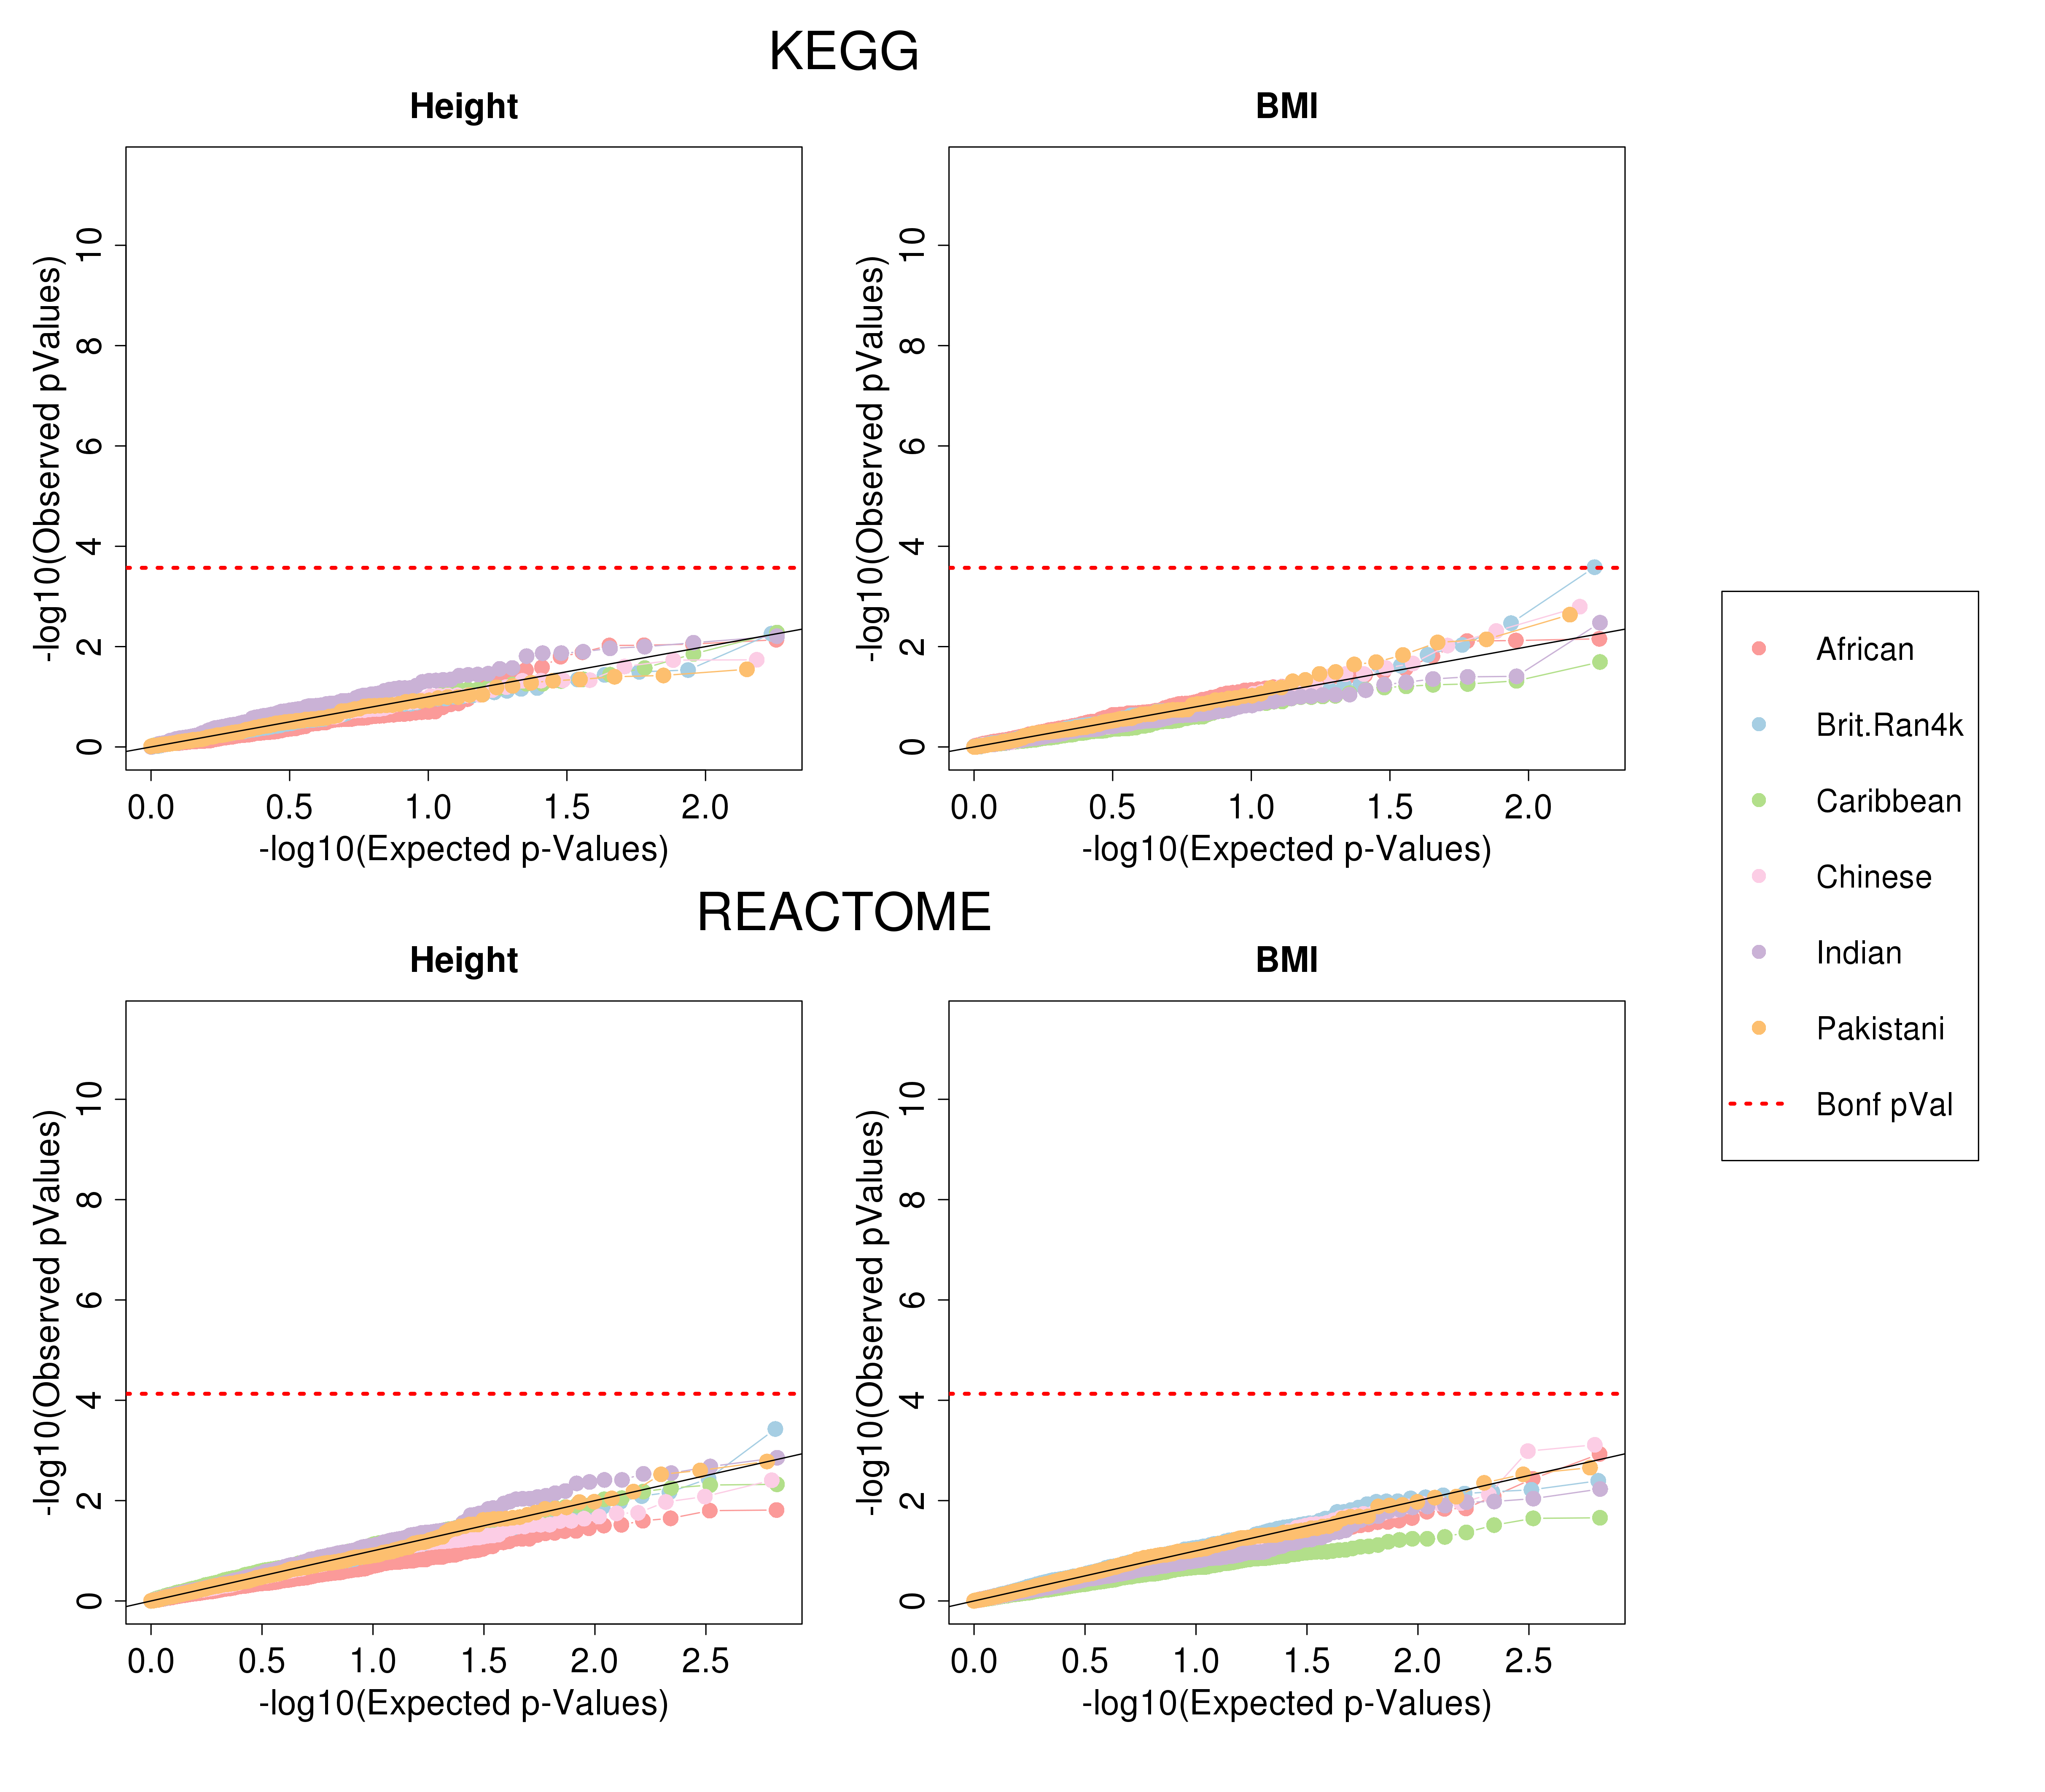
\includegraphics[width = \textwidth]{Images/Supp/InterPath_Supp_Figure_perm1_QQPlots_AllPaths_vs2.png}
\caption{\textbf{QQ-Plots of MAPIT-R $\bm{p}$-values using KEGG and REACTOME pathways annotations and randomly permuted phenotypes in each ancestry-specific subgroup in the UK Biobank.} Here, we run MAPIT-R after conducting a single random permutation of either height or BMI measurements. Note that traits were permuted within each population subgroup ten different times. Shown on the x-axis are the -$\log_{10}$ transformed expected $p$-values, while the $y$-axis shows the -$\log_{10}$ observed $p$-values. The dotted red line is the Bonferroni-corrected $P$-value threshold based on the number of pathways tested per database-phenotype combination (Supplementary Table \ref{InterPath-Supp-Table-UKBPopStats}). Subgroups in the UK Biobank included individuals based on their self-identified ancestries: ``African'', ``British'', ``Caribbean'', ``Chinese'', ``Indian'', and ``Pakistani'', respectively. Overall, we find that MAPIT-R properly controls for type 1 error rate at varying significance cutoff thresholds (Supplementary Table \ref{InterPath-Supp-Table-AllPops-FDRs}).}
\label{InterPath-Supp-Figure-perm1-QQPlots-AllPaths}
\end{figure}
\clearpage

%\setlength{\footskip}{3cm}
\begin{figure}[htbp]
\centering
\vspace*{-2cm}
\includegraphics[width = \textwidth]{Images/Supp/InterPath_Supp_Figure_pValHists_vs3.png}
\caption{\textbf{Histograms of MAPIT-R $\bm{p}$-values using KEGG and REACTOME pathways annotations and randomly permuted phenotypes in each ancestry-specific subgroup in the UK Biobank.} Here, we run MAPIT-R after conducting a single random permutation of either height or BMI measurements. Note that traits were independently permuted within each population subgroup ten different times. Subgroups in the UK Biobank included individuals based on their self-identified ancestries: ``African'', ``British'', ``Caribbean'', ``Chinese'', ``Indian'', and ``Pakistani'', respectively. Overall, we find that MAPIT-R properly controls for type 1 error rate at varying significance cutoff thresholds (Supplementary Table \ref{InterPath-Supp-Table-AllPops-FDRs}).}
\label{InterPath-Supp-Figure-10perms-pValHists}
\end{figure}
\clearpage
\setlength{\footskip}{1cm}

\setlength{\footskip}{1cm}
\begin{figure}[htbp]
\centering
%\vspace*{-2cm}
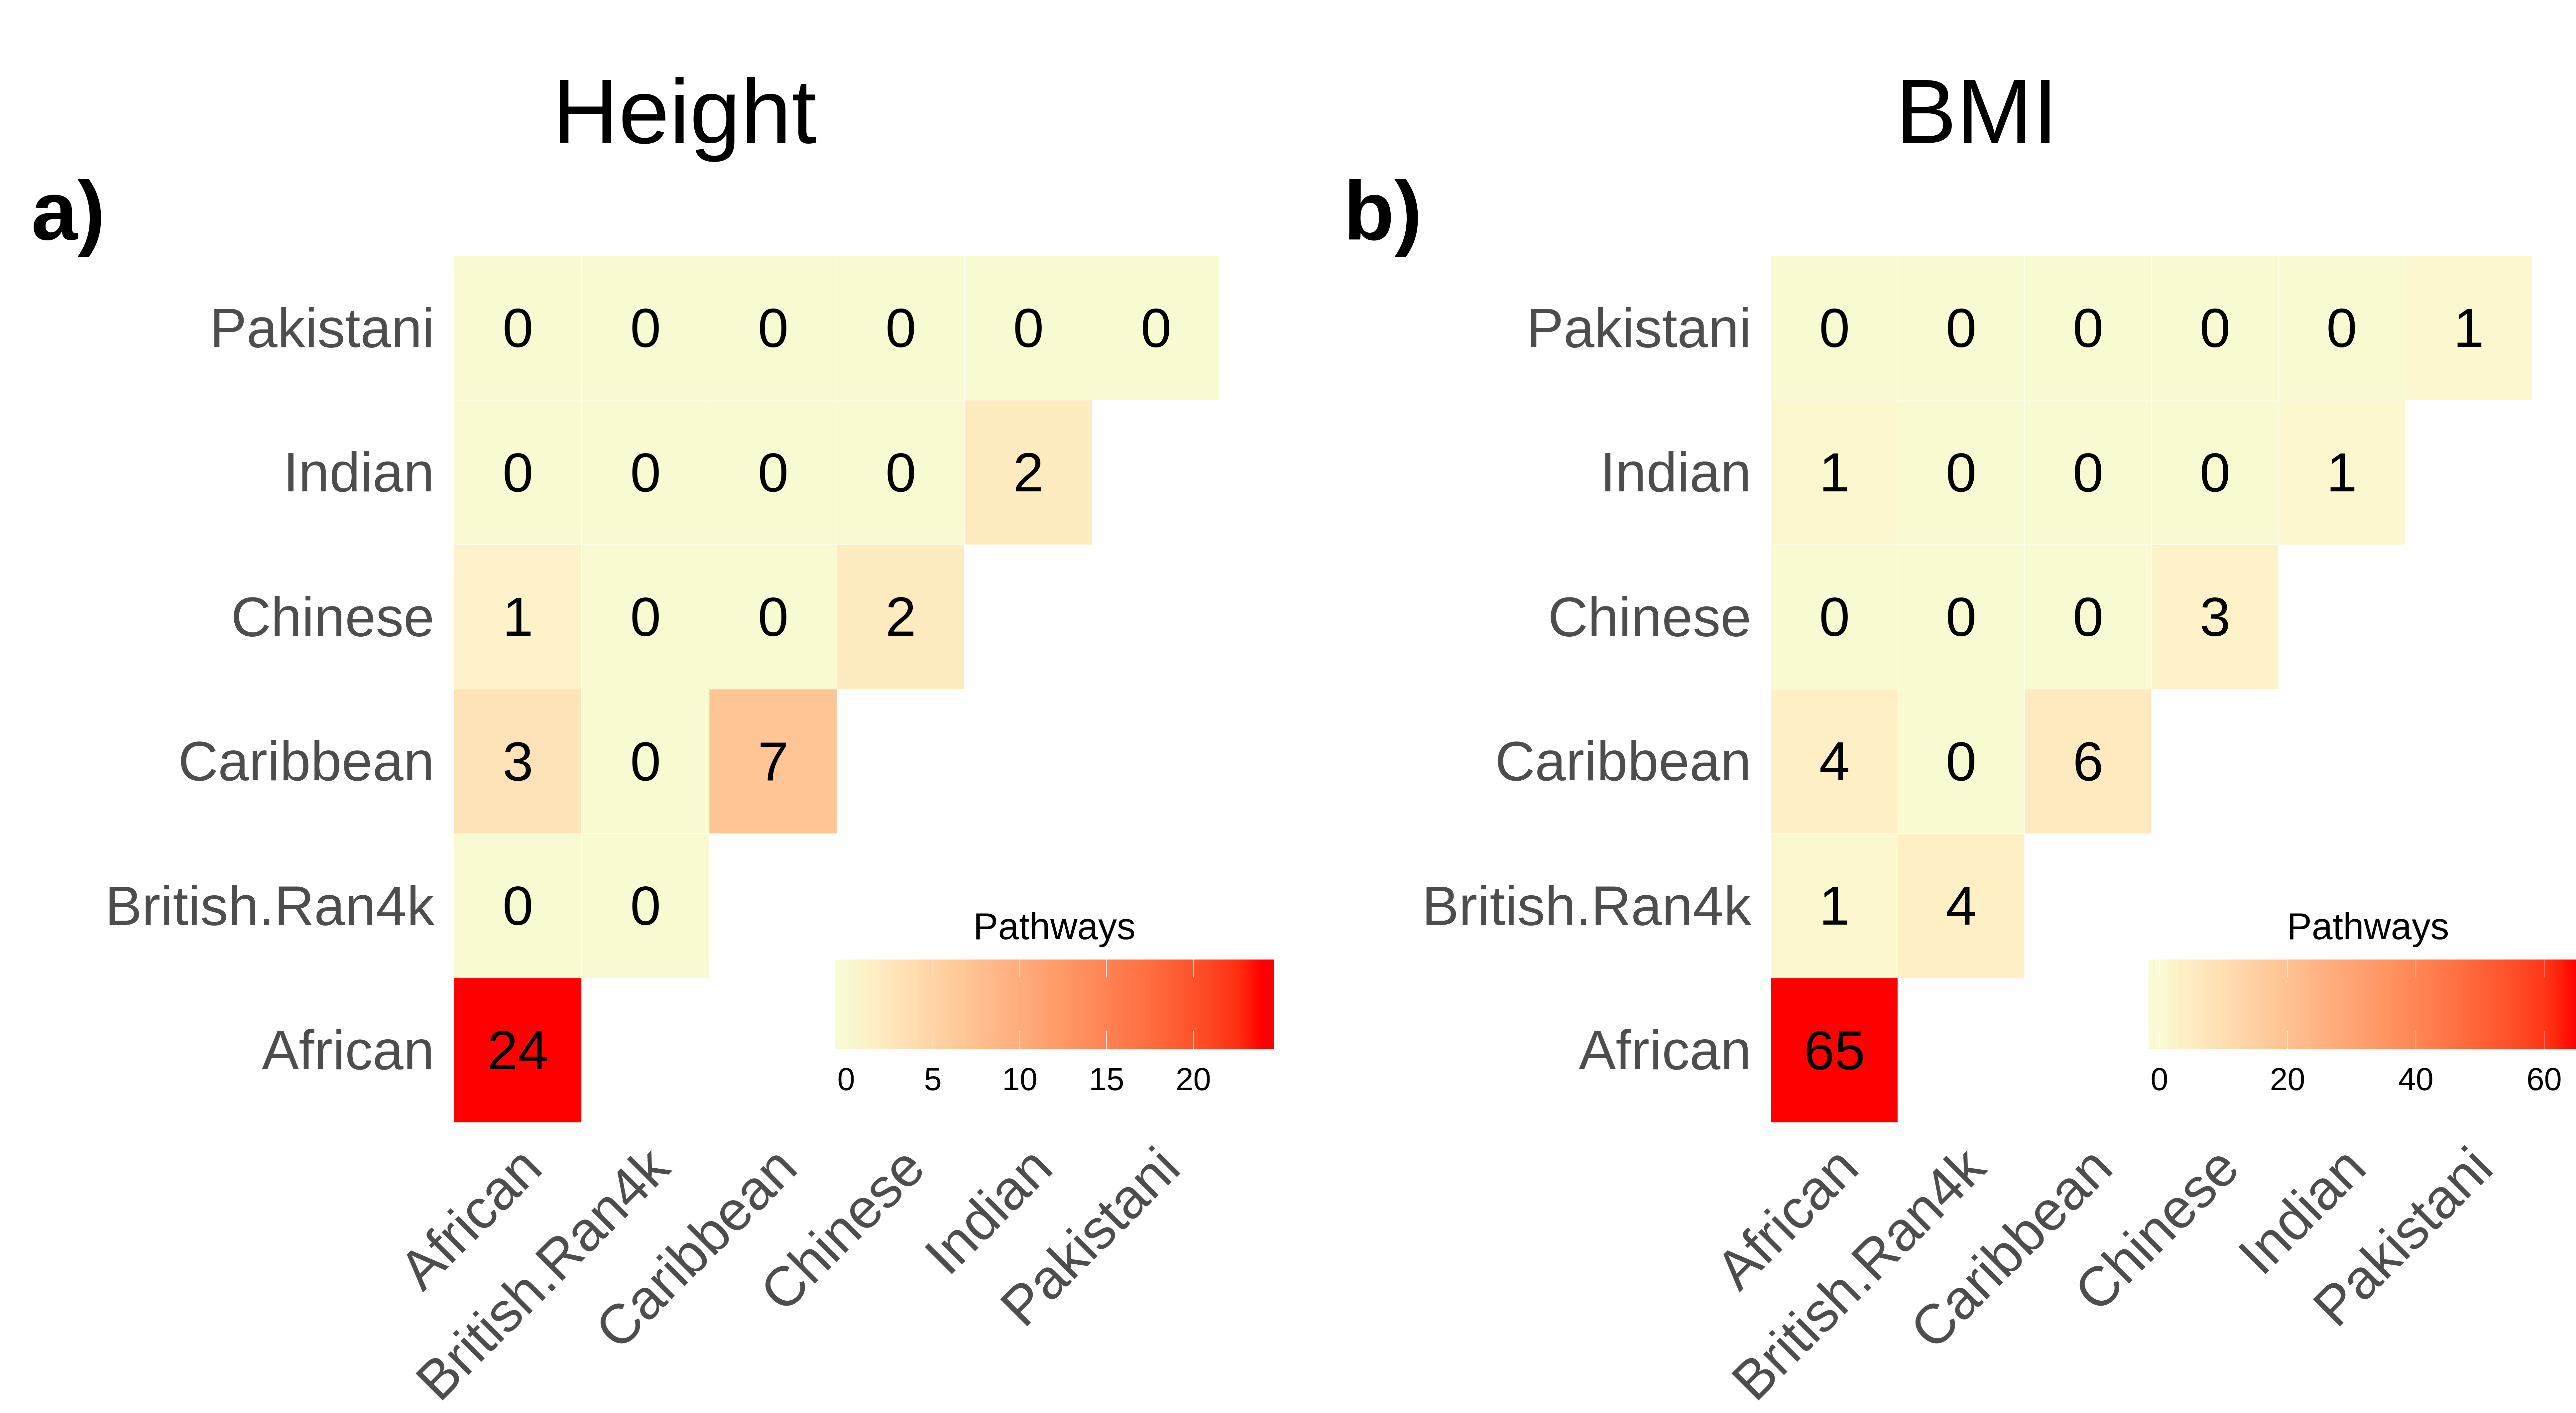
\includegraphics[width = \textwidth]{Images/Supp/InterPath_Supp_Figure_Heatplots_REACTOME_vs4.png}
\caption{\textbf{Heatmaps depicting the overlap of MAPIT-R significant REACTOME pathways for (a) standing height and (b) body mass index (BMI) between the different ancestry-specific subgroups in the UK Biobank}. Here, subgroups in the UK Biobank included individuals based on their self-identified ancestries: ``African'', ``British'', ``Caribbean'', ``Chinese'', ``Indian'', and ``Pakistani'', respectively. Genome-wide significance was determined by using Bonferroni-corrected $P$-value thresholds based on the number of pathways tested in each database-phenotype-subgroup combination (see Supplementary Table \ref{InterPath-Supp-Table-UKBPopStats}). The diagonal shows the total number of genome-wide significant pathways per subgroup. We observe that significant pathways observed in non-African subgroups overlap more often with pathways from the African subgroup than they do with pathways from the other, remaining non-African subgroups. Results for both phenotypes in the KEGG database can be seen in Figure \ref{InterPath-Main-Figure-Heatplots-KEGG} in the main text.}
\label{InterPath-Supp-Figure-Heatplots-REACTOME}
\end{figure}
\clearpage
\setlength{\footskip}{1cm}

\begin{landscape}
\setlength{\footskip}{3cm}
\begin{figure}[htbp]
\centering
\hspace*{-2cm}
\includegraphics[angle=270,scale=.25]{Images/Supp/InterPath_Supp_Figure_MAPITR_PhenoComps_AllPops_vs4.png}
\caption{\textbf{Scatterplots comparing the MAPIT-R $\bm{p}$-values using (top) KEGG and (bottom) REACTOME pathways annotations in height and body mass index (BMI) within all of the different ancestry-specific subgroups in the UK Biobank.} Here, subgroups in the UK Biobank included individuals based on their self-identified ancestries: ``African'', ``British'', ``Caribbean'', ``Chinese'', ``Indian'', and ``Pakistani'', respectively. For each plot, the x-axis depicts the -$\log_{10}$ transformed MAPIT-R $p$-value for height, while the y-axis shows the same results for BMI. The red horizontal and vertical dashed lines are marked at the Bonferroni-corrected $p$-value thresholds for genome-wide significance in each pathway-phenotype combination (see Supplementary Table \ref{InterPath-Supp-Table-UKBPopStats}). Pathways in the top right quadrant have significant marginal epistatic effects in both traits; while, points in the bottom right and top left quadrants are pathways that are uniquely enriched in height or BMI, respectively. Within each plot we also list the Pearson correlation coefficient describing the similarity of marginally epistatic enriched pathways in both traits.}
\label{InterPath-Supp-Figure-MAPITR-PhenoComps-AllPops}
\end{figure}
\clearpage
\setlength{\footskip}{1cm}
\end{landscape}

\begin{figure}[htbp]
\centering
\hspace*{-1.75cm}
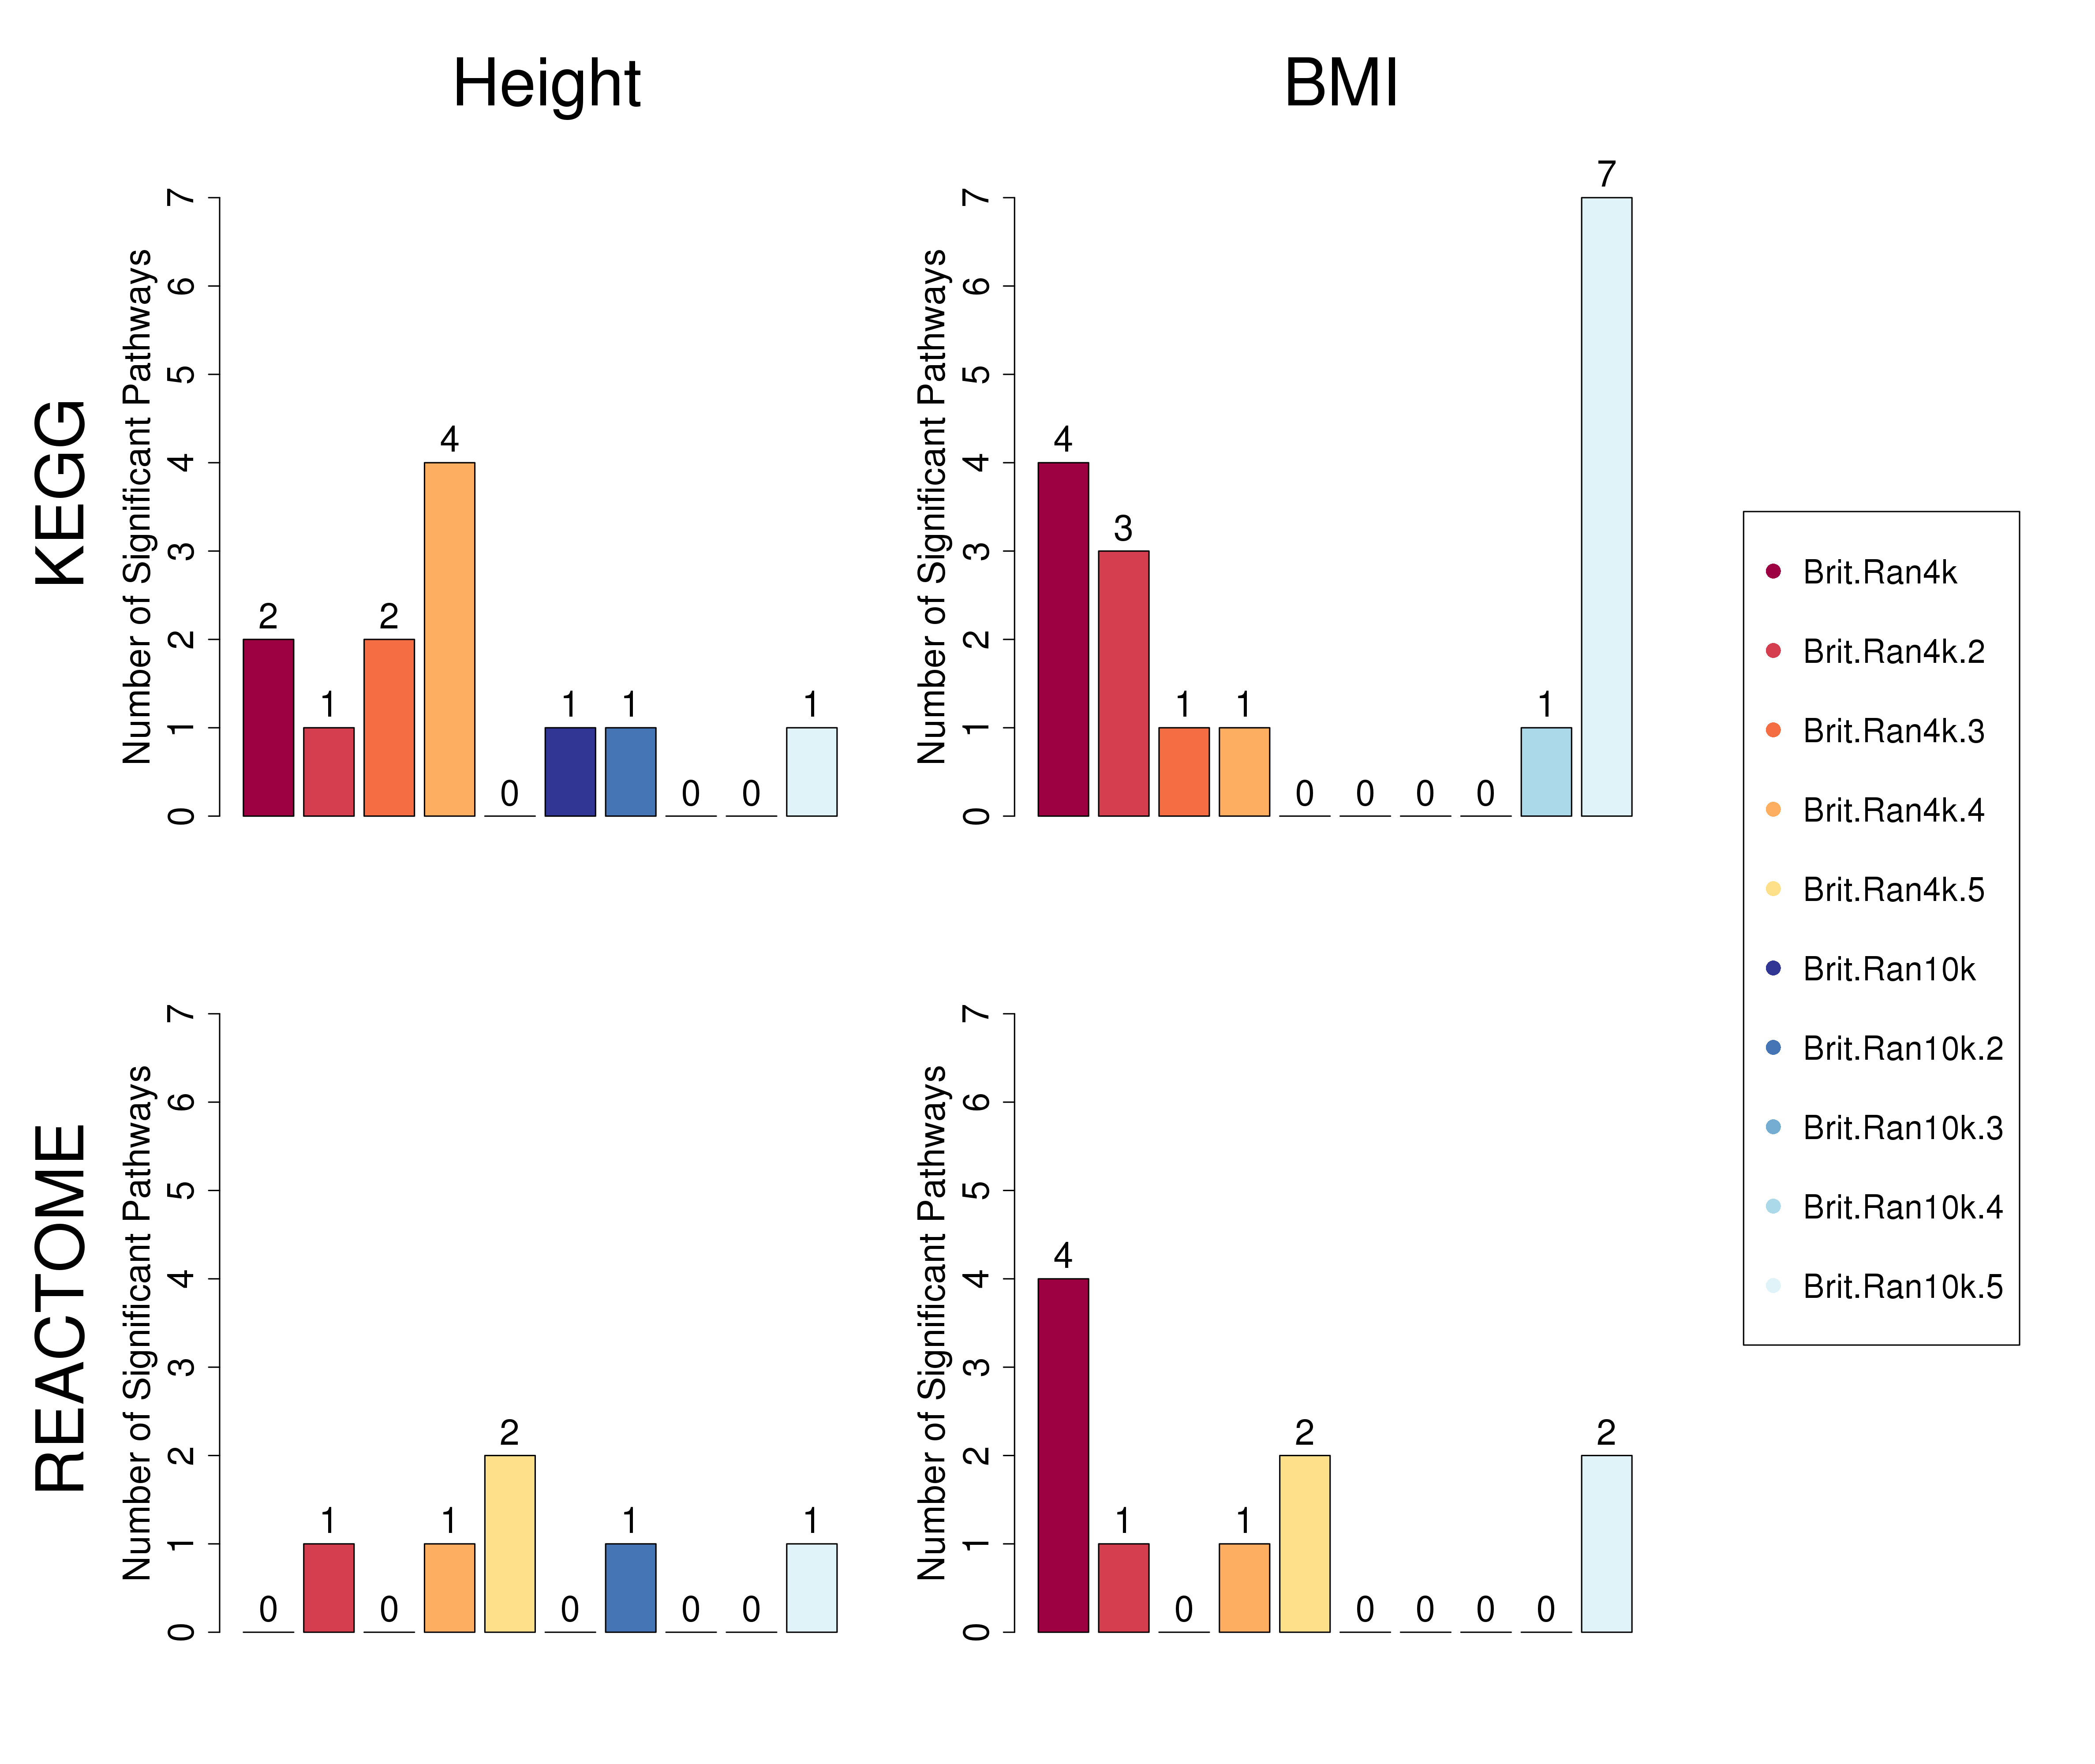
\includegraphics[scale=.45]{Images/Supp/InterPath_Supp_Figure_BritReps_Barplot_vs4.png}
\caption{\textbf{Number of KEGG and REACTOME pathways identified by MAPIT-R that have significant marginal epistatic effects within standing height and body mass index (BMI) per British replicate subgroup in the UK Biobank.} Here, the random subgroups were created by subsampling either $N =$ 4,000 or 10,000 individuals from the full British cohort. In the legend, replicates are marked as numbers after the root tag name (e.g., \texttt{Brit.Ran4k.4} denotes the fourth replicate in the $N =$ 4,000 subsampling scheme). Genome-wide significance was determined by using Bonferroni-corrected $p$-value thresholds based on the number of pathways tested in each database-phenotype-subgroup combination (see Supplementary Table \ref{InterPath-Supp-Table-UKBPopStats}). Note that most replicate runs did not produce many significant results.}
\label{InterPath-Supp-Figure-BritReps-Barplots}
\end{figure}
\clearpage

%\newcounter{CharNumber4}
%\setcounter{CharNumber4}{1}
%\renewcommand{\thefigure}{\arabic{figure}\alph{CharNumber4}}
\begin{landscape}
\begin{figure}[htbp]
\centering
\includegraphics[scale=.2]{Images/Supp/InterPath_Supp_Figure_BritReps_Heatplots_KEGG_vs4.png}
\caption{\textbf{Heatmaps depicting the overlap of MAPIT-R significant KEGG pathways for (a) standing height and (b) body mass index (BMI) per British replicate subgroup in the UK Biobank}. Here, the random subgroups were created by subsampling either $N =$ 4,000 or 10,000 individuals from the full British cohort. In the legend, replicates are marked as numbers after the root tag name (e.g., \texttt{Brit.Ran4k.4} denotes the fourth replicate in the $N =$ 4,000 subsampling scheme). Genome-wide significance was determined by using Bonferroni-corrected $P$-value thresholds based on the number of pathways tested in each database-phenotype-subgroup combination (see Supplementary Table \ref{InterPath-Supp-Table-UKBPopStats}). The diagonal shows the total number of genome-wide significant pathways per subgroup. We do not observe much overlap between enriched pathways between the replicate subgroups --- even though they all consist of individuals of the same ancestry.}
\label{InterPath-Supp-Figure-BritReps-Heatplots-AllPaths-KEGG}
\end{figure}
\clearpage
%\addtocounter{figure}{-1}
%\addtocounter{CharNumber4}{1}
\end{landscape}

\begin{landscape}
\begin{figure}[htbp]
\centering
\includegraphics[scale=.2]{Images/Supp/InterPath_Supp_Figure_BritReps_Heatplots_REACTOME_vs4.png}
\caption{\textbf{Heatmaps depicting the overlap of MAPIT-R significant REACTOME pathways for (a) standing height and (b) body mass index (BMI) per British replicate subgroup in the UK Biobank}. Here, the random subgroups were created by subsampling either $N =$ 4,000 or 10,000 individuals from the full British cohort. In the legend, replicates are marked as numbers after the root tag name (e.g., \texttt{Brit.Ran4k.4} denotes the fourth replicate in the $N =$ 4,000 subsampling scheme). Genome-wide significance was determined by using Bonferroni-corrected $P$-value thresholds based on the number of pathways tested in each database-phenotype-subgroup combination (see Supplementary Table \ref{InterPath-Supp-Table-UKBPopStats}). The diagonal shows the total number of genome-wide significant pathways per subgroup. We do not observe much overlap between enriched pathways between the replicate subgroups --- even though they all consist of individuals of the same ancestry.}
\label{InterPath-Supp-Figure-BritReps-Heatplots-AllPaths-REACTOME}
\end{figure}
\clearpage
\end{landscape}
%\renewcommand{\thefigure}{\arabic{figure}}

\begin{figure}[htbp]
\centering
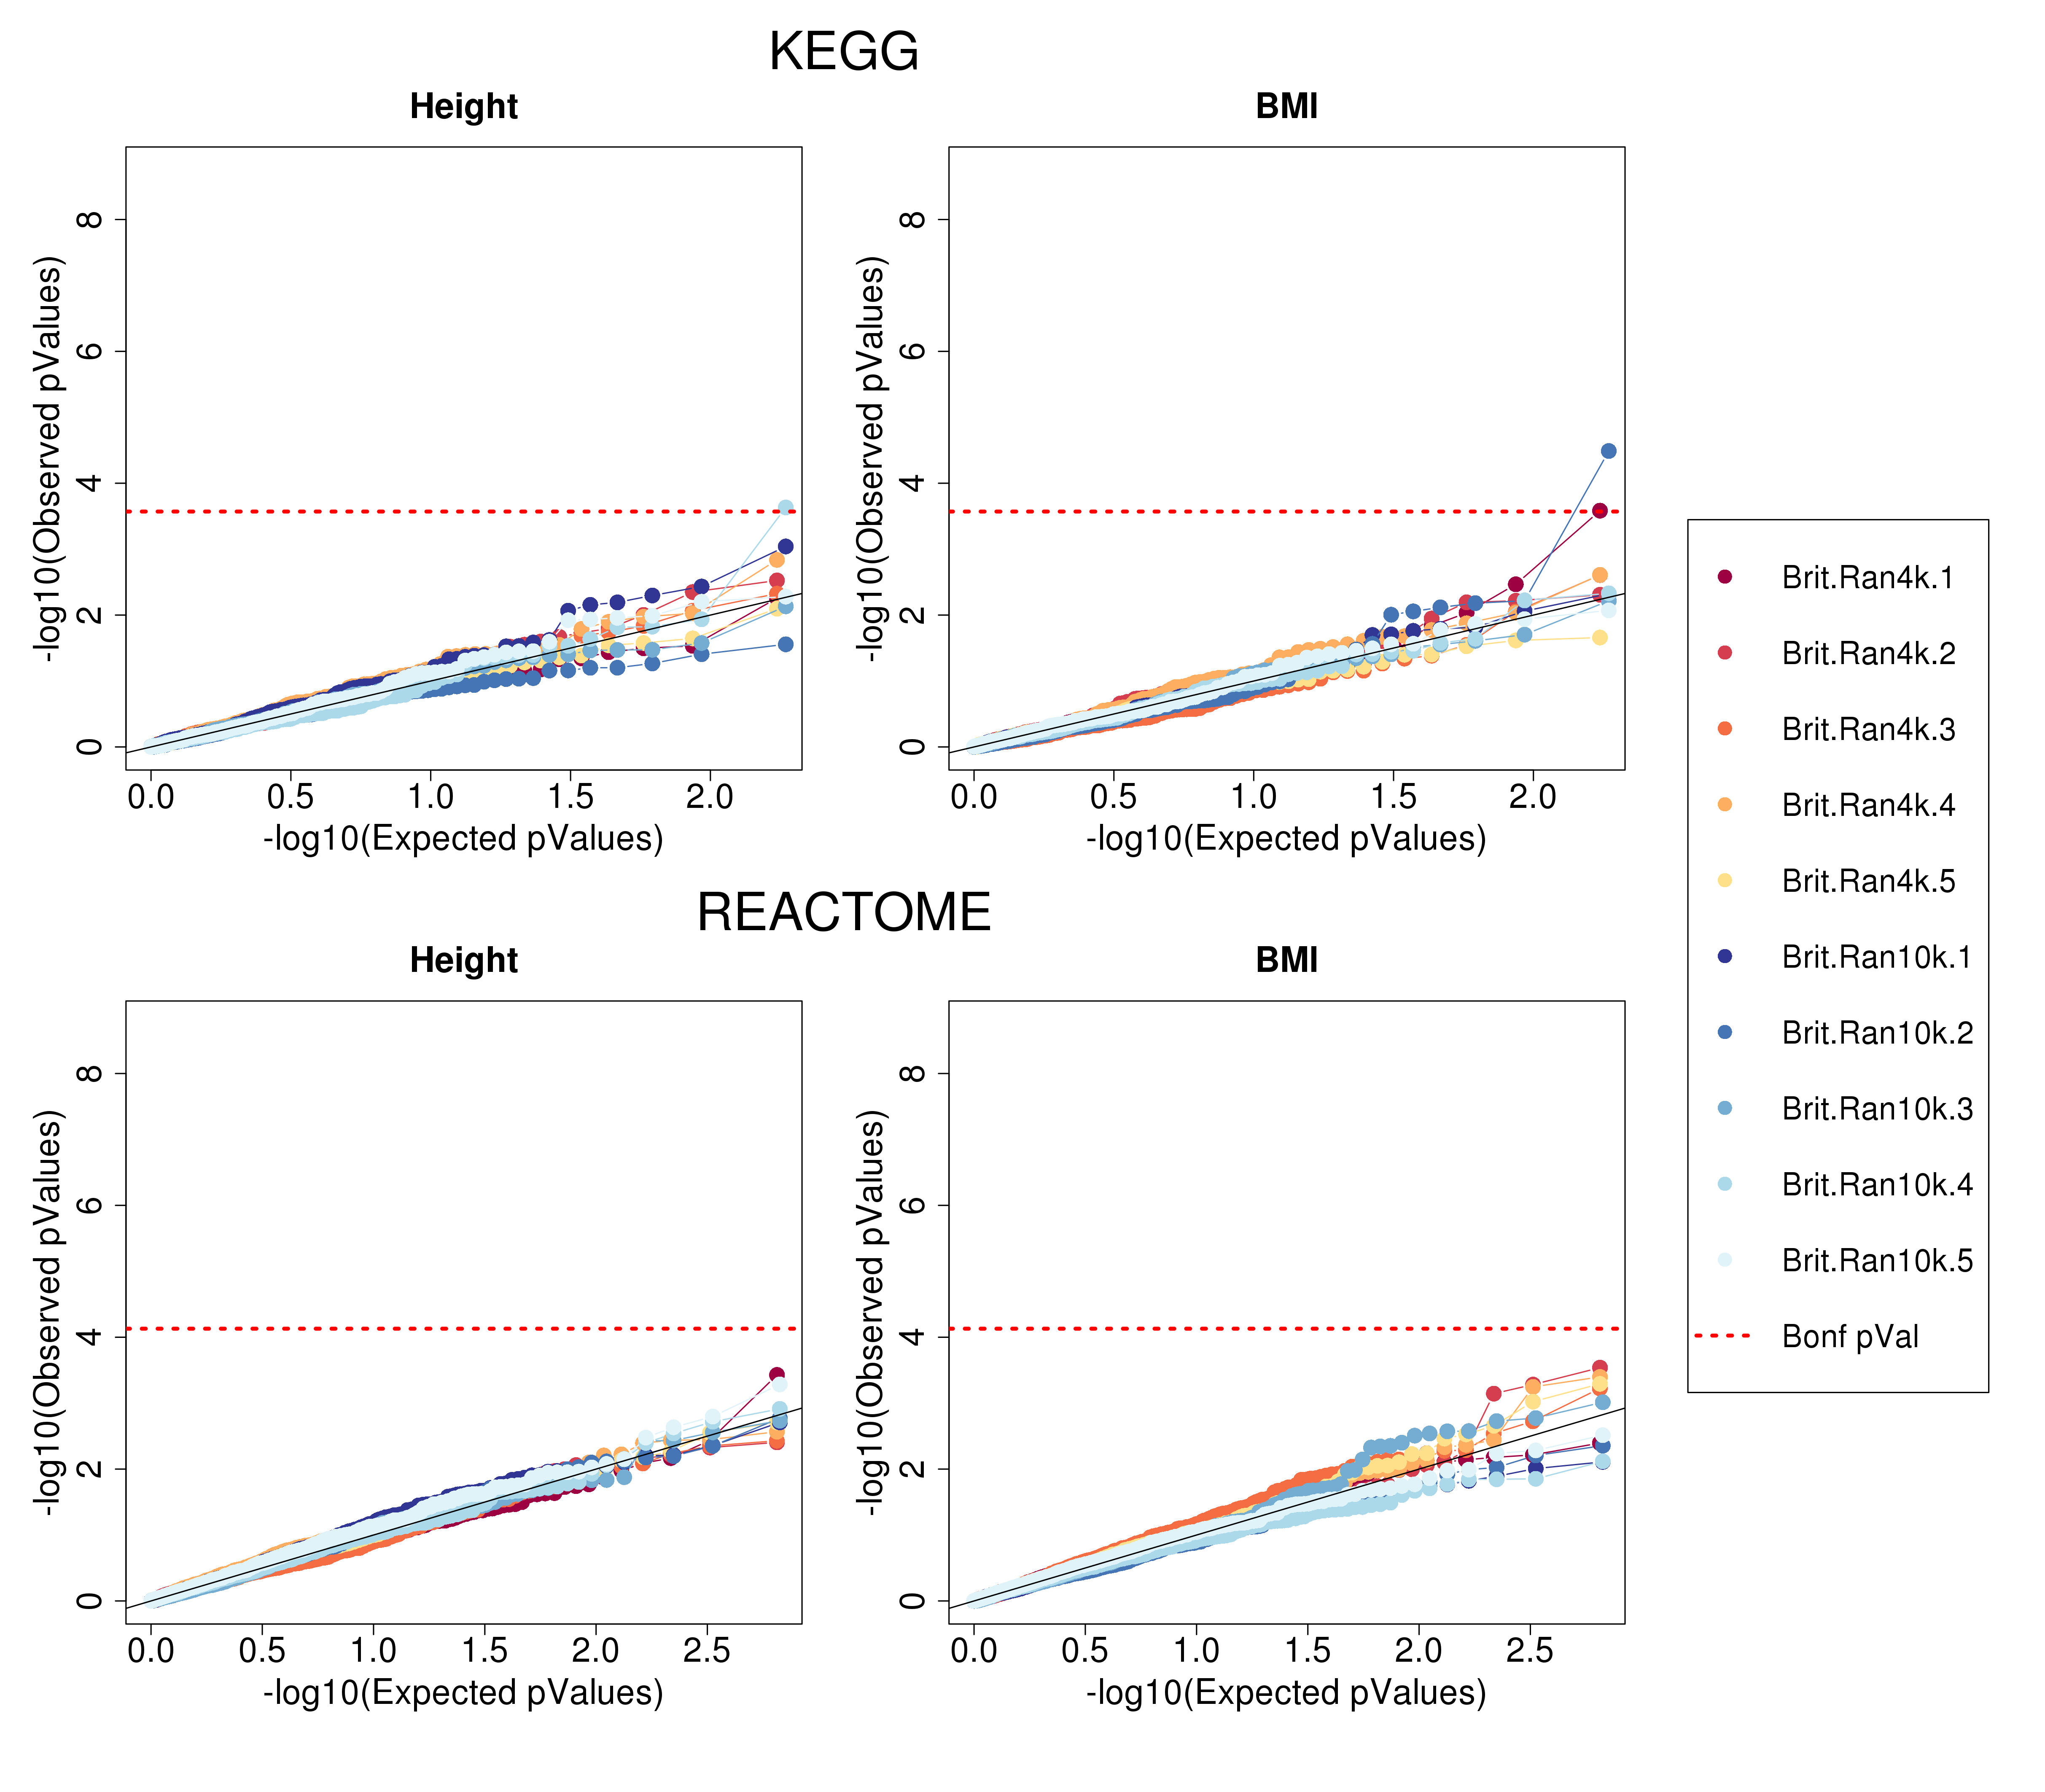
\includegraphics[width=\textwidth]{Images/Supp/InterPath_Supp_Figure_BritReps_perm1_QQPlots_AllPaths_vs1.png}
\caption{\textbf{QQ-Plots of MAPIT-R $\bm{p}$-values using KEGG and REACTOME pathways annotations and randomly permuted phenotypes in British replicate subgroups from the UK Biobank.} Here, we run MAPIT-R after conducting a single random permutation of either height or BMI measurements. Note that traits were permuted within each population subgroup ten different times. Shown on the x-axis are the -$\log_{10}$ transformed expected $p$-values, while the $y$-axis shows the -$\log_{10}$ observed $p$-values. The random subgroups were created by subsampling either $N =$ 4,000 or 10,000 individuals from the full British cohort. In the legend, replicates are marked as numbers after the root tag name (e.g., \texttt{Brit.Ran4k.4} denotes the fourth replicate in the $N =$ 4,000 subsampling scheme). The dotted red line is the Bonferroni-corrected $P$-value threshold based on the number of pathways tested per database-phenotype combination (Supplementary Table \ref{InterPath-Supp-Table-UKBPopStats}). Overall, we find that MAPIT-R continues to exhibit well-calibrated behavior under the null hypothesis and properly controls for type 1 error rate.}
\label{InterPath-Supp-Figure-BritReps-perm1-QQPlots-AllPaths}
\end{figure}
\clearpage

%\newcounter{CharNumber3}
%\setcounter{CharNumber3}{1}
%\renewcommand{\thefigure}{\arabic{figure}\alph{CharNumber3}}
%\setlength{\footskip}{1cm}
\begin{figure}[htbp]
\centering
%\vspace*{-1cm}
\includegraphics[width=\textwidth]{Images/Supp/InterPath_Supp_Figure_BritReps_pValHists_AllPaths_vs1_pt1.png}
\caption{\textbf{Histograms of MAPIT-R $\bm{p}$-values using KEGG and REACTOME pathways annotations and randomly permuted phenotypes in each \textcolor{red}{British 4,000 replicate} subgroup in the UK Biobank.} Here, we run MAPIT-R after conducting a single random permutation of either height or BMI measurements. Note that traits were independently permuted within each population subgroup ten different times. The random subgroups were created by subsampling $N =$ 4,000 individuals from the full British cohort. In the legend, replicates are marked as numbers after the root tag name (e.g., \texttt{Brit.Ran4k.4} denotes the fourth replicate in the $N =$ 4,000 subsampling scheme). Overall, we find that MAPIT-R continues to exhibit well-calibrated behavior under the null hypothesis.}
\label{InterPath-Supp-Figure-BritReps-10perms-pValHists-pt1}
\end{figure}
\clearpage
%\setlength{\footskip}{1cm}
%\addtocounter{figure}{-1}
%\addtocounter{CharNumber3}{1}

%\setlength{\footskip}{2cm}
\begin{figure}[htbp]
\centering
%\vspace*{-1cm}
\includegraphics[width=\textwidth]{Images/Supp/InterPath_Supp_Figure_BritReps_pValHists_AllPaths_vs1_pt2.png}
\caption{\textbf{Histograms of MAPIT-R $\bm{P}$-values using KEGG and REACTOME pathways annotations and randomly permuted phenotypes in each \textcolor{red}{British 10,000 replicate} subgroup in the UK Biobank.} Here, we run MAPIT-R after conducting a single random permutation of either height or BMI measurements. Note that traits were independently permuted within each population subgroup ten different times. The random subgroups were created by subsampling $N =$ 10,000 individuals from the full British cohort. In the legend, replicates are marked as numbers after the root tag name (e.g., \texttt{Brit.Ran10k.4} denotes the fourth replicate in the $N =$ 10,000 subsampling scheme). Overall, we find that MAPIT-R continues to exhibit well-calibrated behavior under the null hypothesis.}
\label{InterPath-Supp-Figure-BritReps-10perms-pValHists-pt2}
\end{figure}
\clearpage
%\setlength{\footskip}{1cm}
%\renewcommand{\thefigure}{\arabic{figure}}

%\setlength{\footskip}{3cm}
\begin{landscape}
\begin{figure}[htbp]
\centering
\vspace*{-2.2cm}
\includegraphics[angle=270,scale=0.179]{Images/Supp/InterPath_Supp_Figure_pValsVsNumSNPs_vs3.png}
\caption{\textbf{Scatterplots comparing the MAPIT-R $\bm{P}$-values as function of the number of SNPs annotated within each pathway for KEGG and REACTOME in height and body mass index (BMI) across each ancestry-specific subgroup in the UK Biobank.} Here, subgroups in the UK Biobank included individuals based on their self-identified ancestries: ``African'', ``British'', ``Caribbean'', ``Chinese'', ``Indian'', and ``Pakistani'', respectively. The dotted red line represents the best fit using a univariate model, and the legend provides the corresponding regression coefficient and its associated $p$-value. We observe that for most combinations there is a significant relationship between the MAPIT-R $p$-value and the number of SNPs present in a pathway. This follows our hypothesis that combining SNPs together in a joint analysis might provide greater power to detect marginal epistasis than analyzing each SNP independently. We note, however, that these results appear to not solely be driven just by the presence or absence of large SNP counts --- conducting this same analysis on one of our sets of permuted phenotypes, we find very few significant relationships between MAPIT-R $p$-values and pathway SNP counts (Supplementary Figure \ref{InterPath-Supp-Figure-pValsVsNumSNPs-perm1}).}
\label{InterPath-Supp-Figure-pValsVsNumSNPs}
\end{figure}
\clearpage
\end{landscape}
%\setlength{\footskip}{1cm}

\begin{landscape}
%\setlength{\footskip}{3cm}
\begin{figure}[htbp]
\centering
\vspace*{-2.2cm}
\includegraphics[angle=270,scale=0.179]{Images/Supp/InterPath_Supp_Figure_pValsVsNumSNPs_perm1_vs3.png}
\caption{\textbf{Scatterplots comparing the MAPIT-R $\bm{P}$-values as function of the number of SNPs annotated within each pathway for KEGG and REACTOME using permuted phenotypes across each ancestry-specific subgroup in the UK Biobank.} Here, we run MAPIT-R after conducting a single random permutation of either height or BMI measurements. Note that traits were independently permuted within each population subgroup ten different times. The dotted red line represents the best fit using a univariate model, and the legend provides the corresponding regression coefficient and its associated $p$-value. Subgroups in the UK Biobank included individuals based on their self-identified ancestries: ``African'', ``British'', ``Caribbean'', ``Chinese'', ``Indian'', and ``Pakistani'', respectively. In these permuted cases, we observe hardly any relationship between MAPIT-R results and the number of SNPs present in a pathway. For this same analysis on the original set of observed phenotypes, see Supplementary Figure \ref{InterPath-Supp-Figure-pValsVsNumSNPs}.}
\label{InterPath-Supp-Figure-pValsVsNumSNPs-perm1}
\end{figure}
\clearpage
%\setlength{\footskip}{1cm}
\end{landscape}

%From: ,https://tex.stackexchange.com/questions/64934/subfig-label-positioning, https://tex.stackexchange.com/questions/196653/how-do-i-stack-two-figures-on-top-of-each-other-rather-than-side-to-side, https://tex.stackexchange.com/questions/47311/include-table-as-a-subfigure, https://tex.stackexchange.com/questions/169541/looking-for-three-images-on-top-of-each-other-with-text-underneath-each, https://tex.stackexchange.com/questions/10863/is-there-a-way-to-slightly-shrink-a-table-including-font-size-to-fit-within-th

%\newcounter{CharNumber5}
%\setcounter{CharNumber5}{1}
%\renewcommand{\thefigure}{\arabic{figure}\alph{CharNumber5}}
%\begin{figure}[ht]
%\centering
%\vspace*{-.5cm}
%\subfloat[]{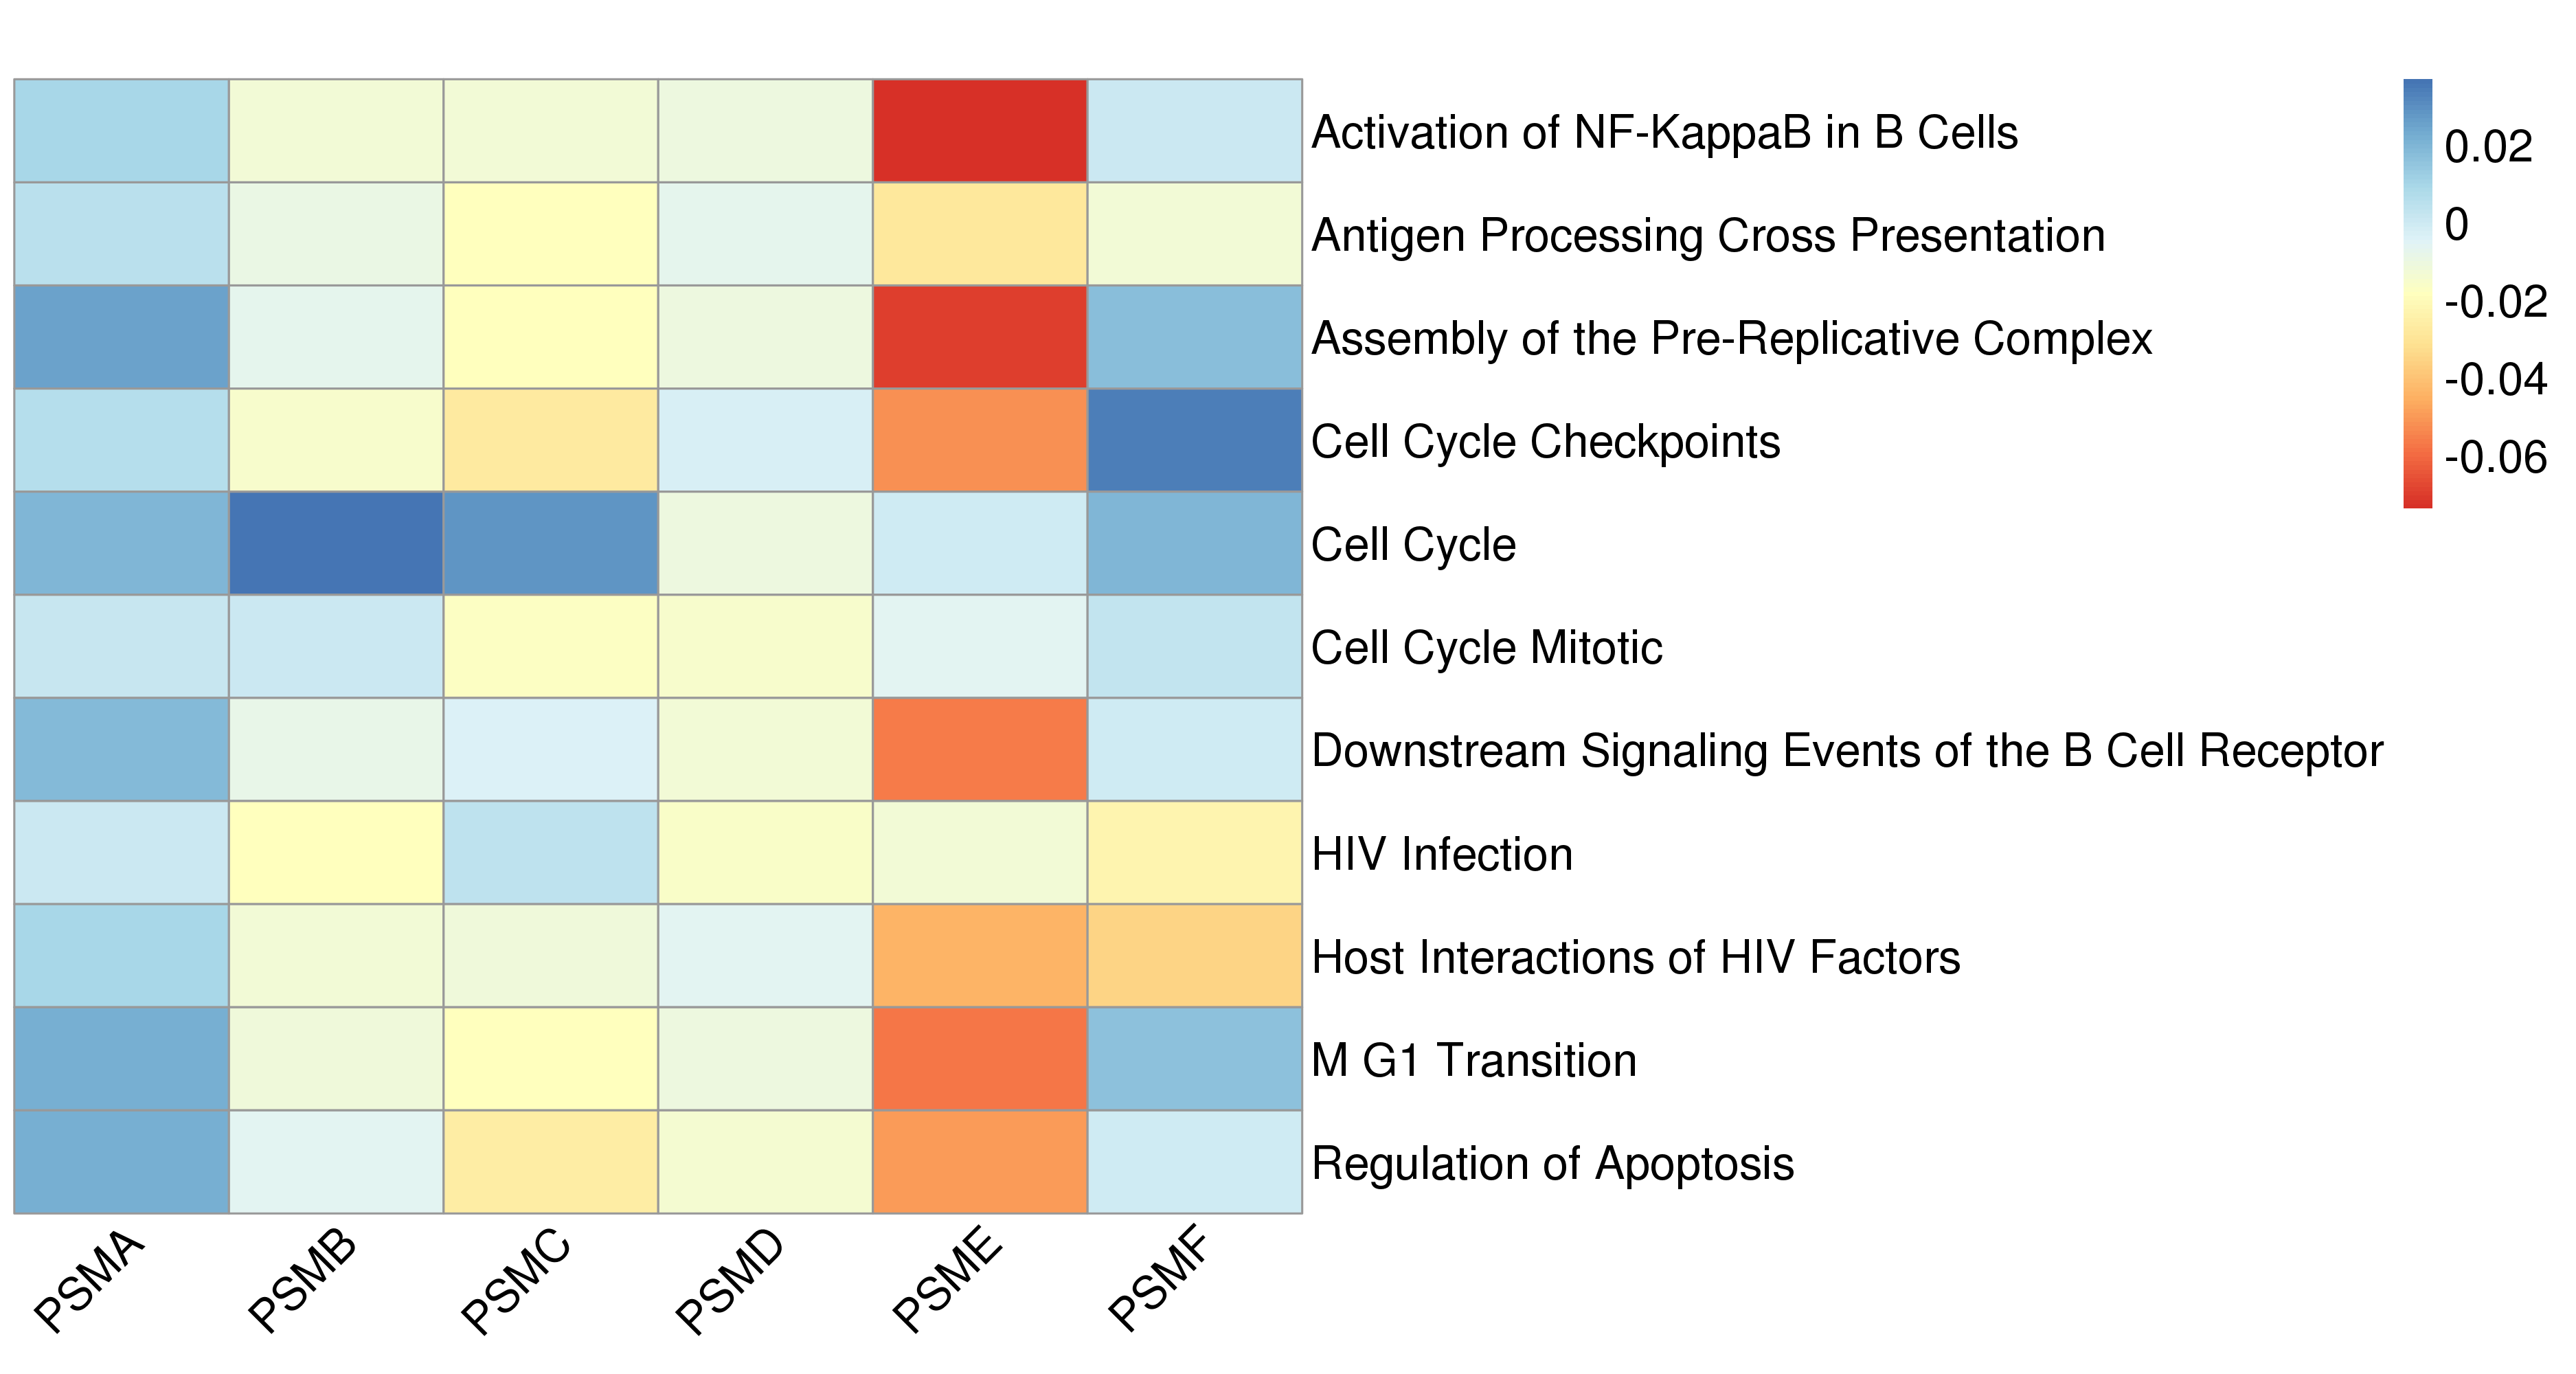
\includegraphics[scale=.5]{Images/Supp/InterPath_Supp_Figure_Proteaseome_Heatplots_African_Loop_vs3.png}}
\par
%\subfloat[]{\resizebox{1.1\columnwidth}{!}{
% \hspace*{-1.75cm}
% \begin{tabular}{cc|ccc}
%  \hline
%\textbf{Proteasome} & \textbf{SNPs} & \textbf{REACTOME} & \textbf{SNPs} & \textbf{MAPIT-R} \\
% \textbf{Gene Family} & & \textbf{Pathway} & & \textbf{$p$-Value} \\
%  \hline
%PSMA & 17 & Activation of NF-KappaB in B Cells & 465 & 1.86E-05  \\
%PSMB & 74 & Antigen Processing Cross Presentation & 850 & 3.96E-05 \\
%PSMC & 20 & Assembly of the Pre-Replicative Complex & 331 & 3.29E-05 \\
%PSMD & 62 & Cell Cycle Checkpoints & 670 & 5.78E-06 \\
%PSME & 15 & Cell Cycle & 2459 & 1.29E-06 \\
%PSMF & 16 & Cell Cycle Mitotic & 1906 & 4.51E-05 \\
% & & Downstream Signaling Events of the B Cell Receptor & 745 & 1.19E-05 \\
% & & HIV Infection & 1346 & 7.53E-07 \\
% & & Host Interactions of HIV Factors & 963 & 7.52E-06 \\
% & & M G1 Transition & 458 & 3.19E-06 \\
% & & Regulation of Apoptosis & 564 & 1.22E-05 \\
%  \hline
%\end{tabular}}}
%\caption[TBD]{\textbf{Proteasome gene family leave-one-out MAPIT-R reruns, REACTOME-BMI-African}. (a) The figure shows the change in original MAPIT-R -$\log_{10}$ $p$-value for each presented REACTOME pathway when each proteasome gene family is removed one at a time. The analyses were conducted in the BMI-African subgroup combination. The $x$-axis shows each proteasome gene family and the $y$-axis shows each REACTOME pathway. Each column has been scaled by the number of SNPs present in the given gene family and, as a result, the heatplot specifically shows the -$\log_{10}$ $p$-value change per SNP. (b) The table shows the number of SNPs that are present in each proteasome gene family (left) and each REACTOME pathway (right). The original MAPIT-R $p$-values for each pathway are also shown (right).}
%\label{InterPath-Supp-Figure-Prot-Heatplots-African}
%\end{figure}
%\clearpage
%\addtocounter{figure}{-1}
%\addtocounter{CharNumber5}{1}

\begin{figure}[H]
\centering
\vspace*{-.5cm}
\subfigure[$\Delta$ in MAPIT-R -$\log_{10}$ $p$-value per SNP]{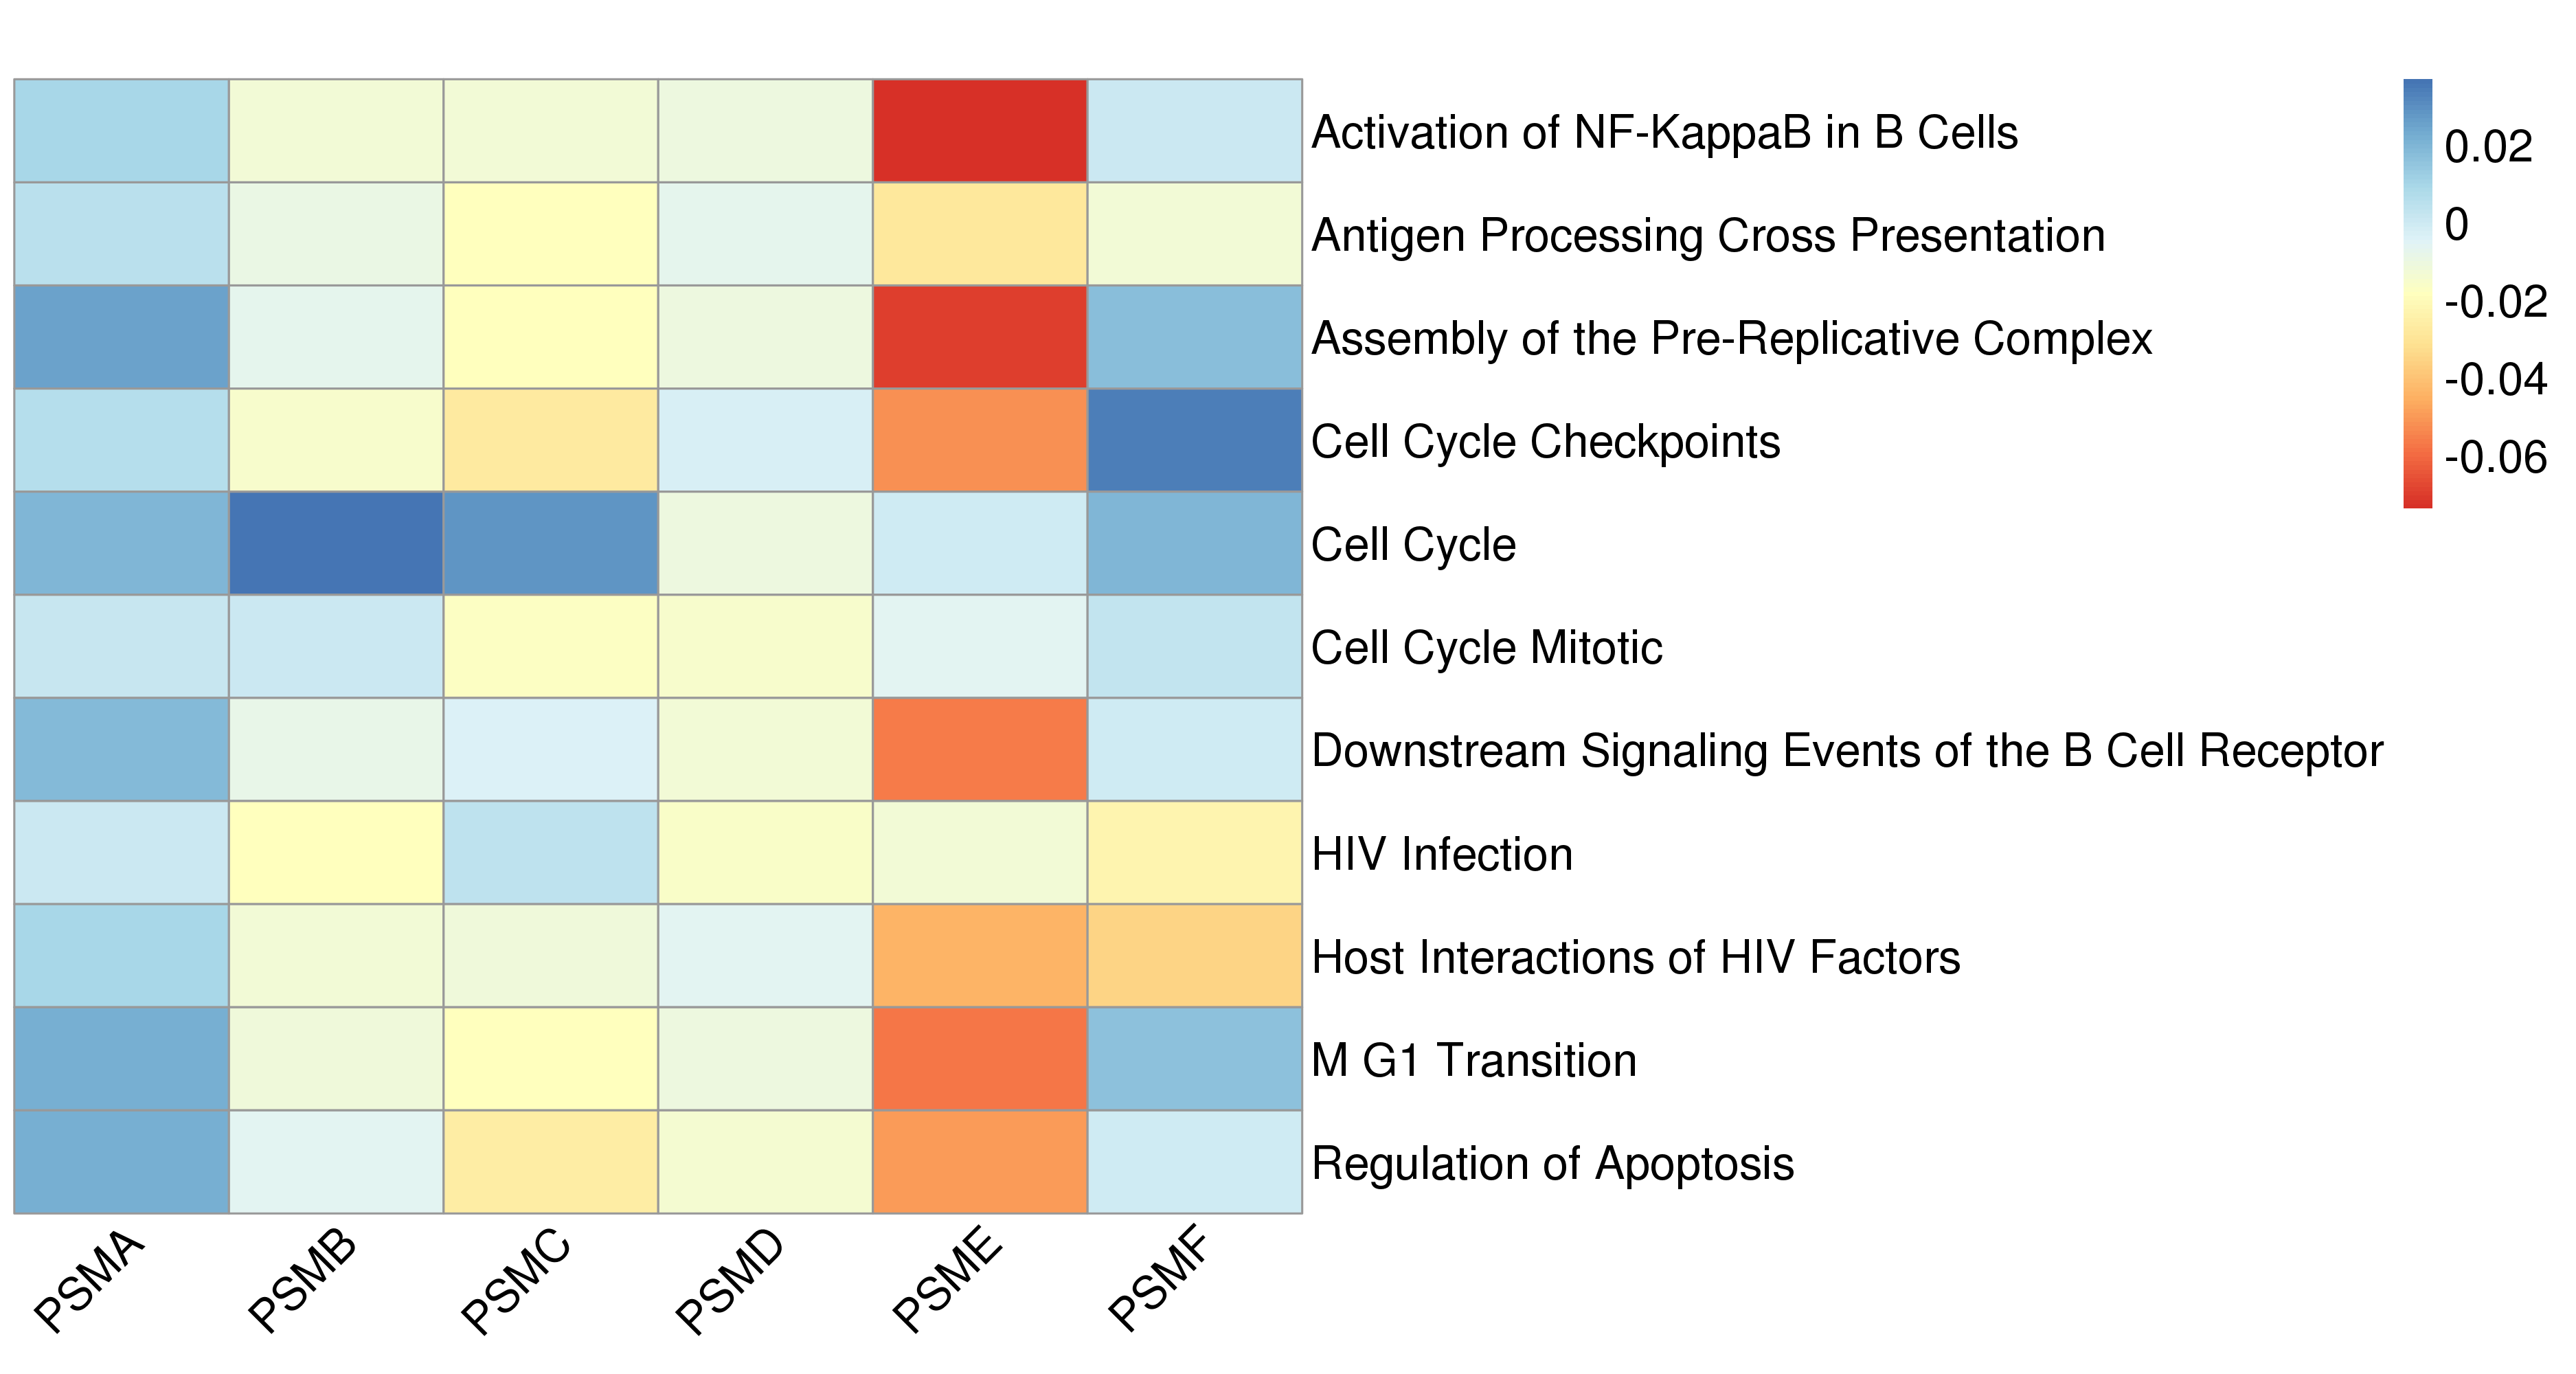
\includegraphics[width=\textwidth]{Images/Supp/InterPath_Supp_Figure_Proteaseome_Heatplots_African_Loop_vs3.png}}
\subfigure[\textcolor{red}{Number of SNPs in each Proteasome Gene Family and REACTOME Pathway}]{
\setlength{\extrarowheight}{3pt}
 \hspace*{-1cm}
 \begin{tabular}{|cc|ccc|}
  \hline
\textbf{Gene Family} & \textbf{\# SNPs} & \textbf{REACTOME Pathway} & \textbf{\# SNPs} & \textbf{$\bm{P}$-Value}\\ [2pt]\hline
PSMA & 17 & Activation of NF-KappaB in B Cells & 465 & 1.86$\times10^{-5}$  \\[2pt]
PSMB & 74 & Antigen Processing Cross Presentation & 850 & 3.96$\times10^{-5}$ \\[2pt]
PSMC & 20 & Assembly of the Pre-Replicative Complex & 331 & 3.29$\times10^{-5}$ \\[2pt]
PSMD & 62 & Cell Cycle Checkpoints & 670 & 5.78$\times10^{-6}$ \\[2pt]
PSME & 15 & Cell Cycle & 2459 & 1.29$\times10^{-6}$\\[2pt]
PSMF & 16 & Cell Cycle Mitotic & 1906 & 4.51$\times10^{-5}$ \\[2pt]
 & & Downstream Signaling Events of the B Cell Receptor & 745 & 1.19$\times10^{-5}$ \\[2pt]
 & & HIV Infection & 1346 & 7.53$\times10^{-7}$ \\[2pt]
 & & Host Interactions of HIV Factors & 963 & 7.52$\times10^{-6}$ \\[2pt]
 & & M G1 Transition & 458 & 3.19$\times10^{-6}$ \\[2pt]
 & & Regulation of Apoptosis & 564 & 1.22$\times10^{-5}$ \\[2pt]
  \hline
\end{tabular}}
\caption{\textbf{Results from applying a ``leave-one-out'' approach to MAPIT-R with proteasome gene families in body mass index (BMI) within the African subgroup in the UK Biobank.} \textbf{(a)} The heatmap shows the change in original MAPIT-R -$\log_{10}$ $P$-value for different REACTOME pathways when each proteasome gene family is removed one at a time in a `leave-one-out' manner. The x-axis shows each proteasome gene family and the y-axis lists each REACTOME pathway. Each column has been scaled by the number of SNPs present in the given gene family and, as a result, the heatmap specifically shows the -$\log_{10}$ $P$-value change per SNP. \textbf{(b)} The table shows the number of SNPs present in each proteasome gene family (left), as well as the number of SNPs present in each REACTOME pathway (right). The original MAPIT-R $P$-values are also shown for each pathway (right).}
\label{InterPath-Supp-Figure-Prot-Heatplots-African}
\end{figure}
\clearpage

%\captionsetup[subfigure]{position=top, labelfont=bf,textfont=normalfont,singlelinecheck=off,justification=raggedright}

\begin{figure}[H]
\centering
\vspace*{-.5cm}
\subfigure[$\Delta$ in MAPIT-R -$\log_{10}$ $p$-value per SNP]{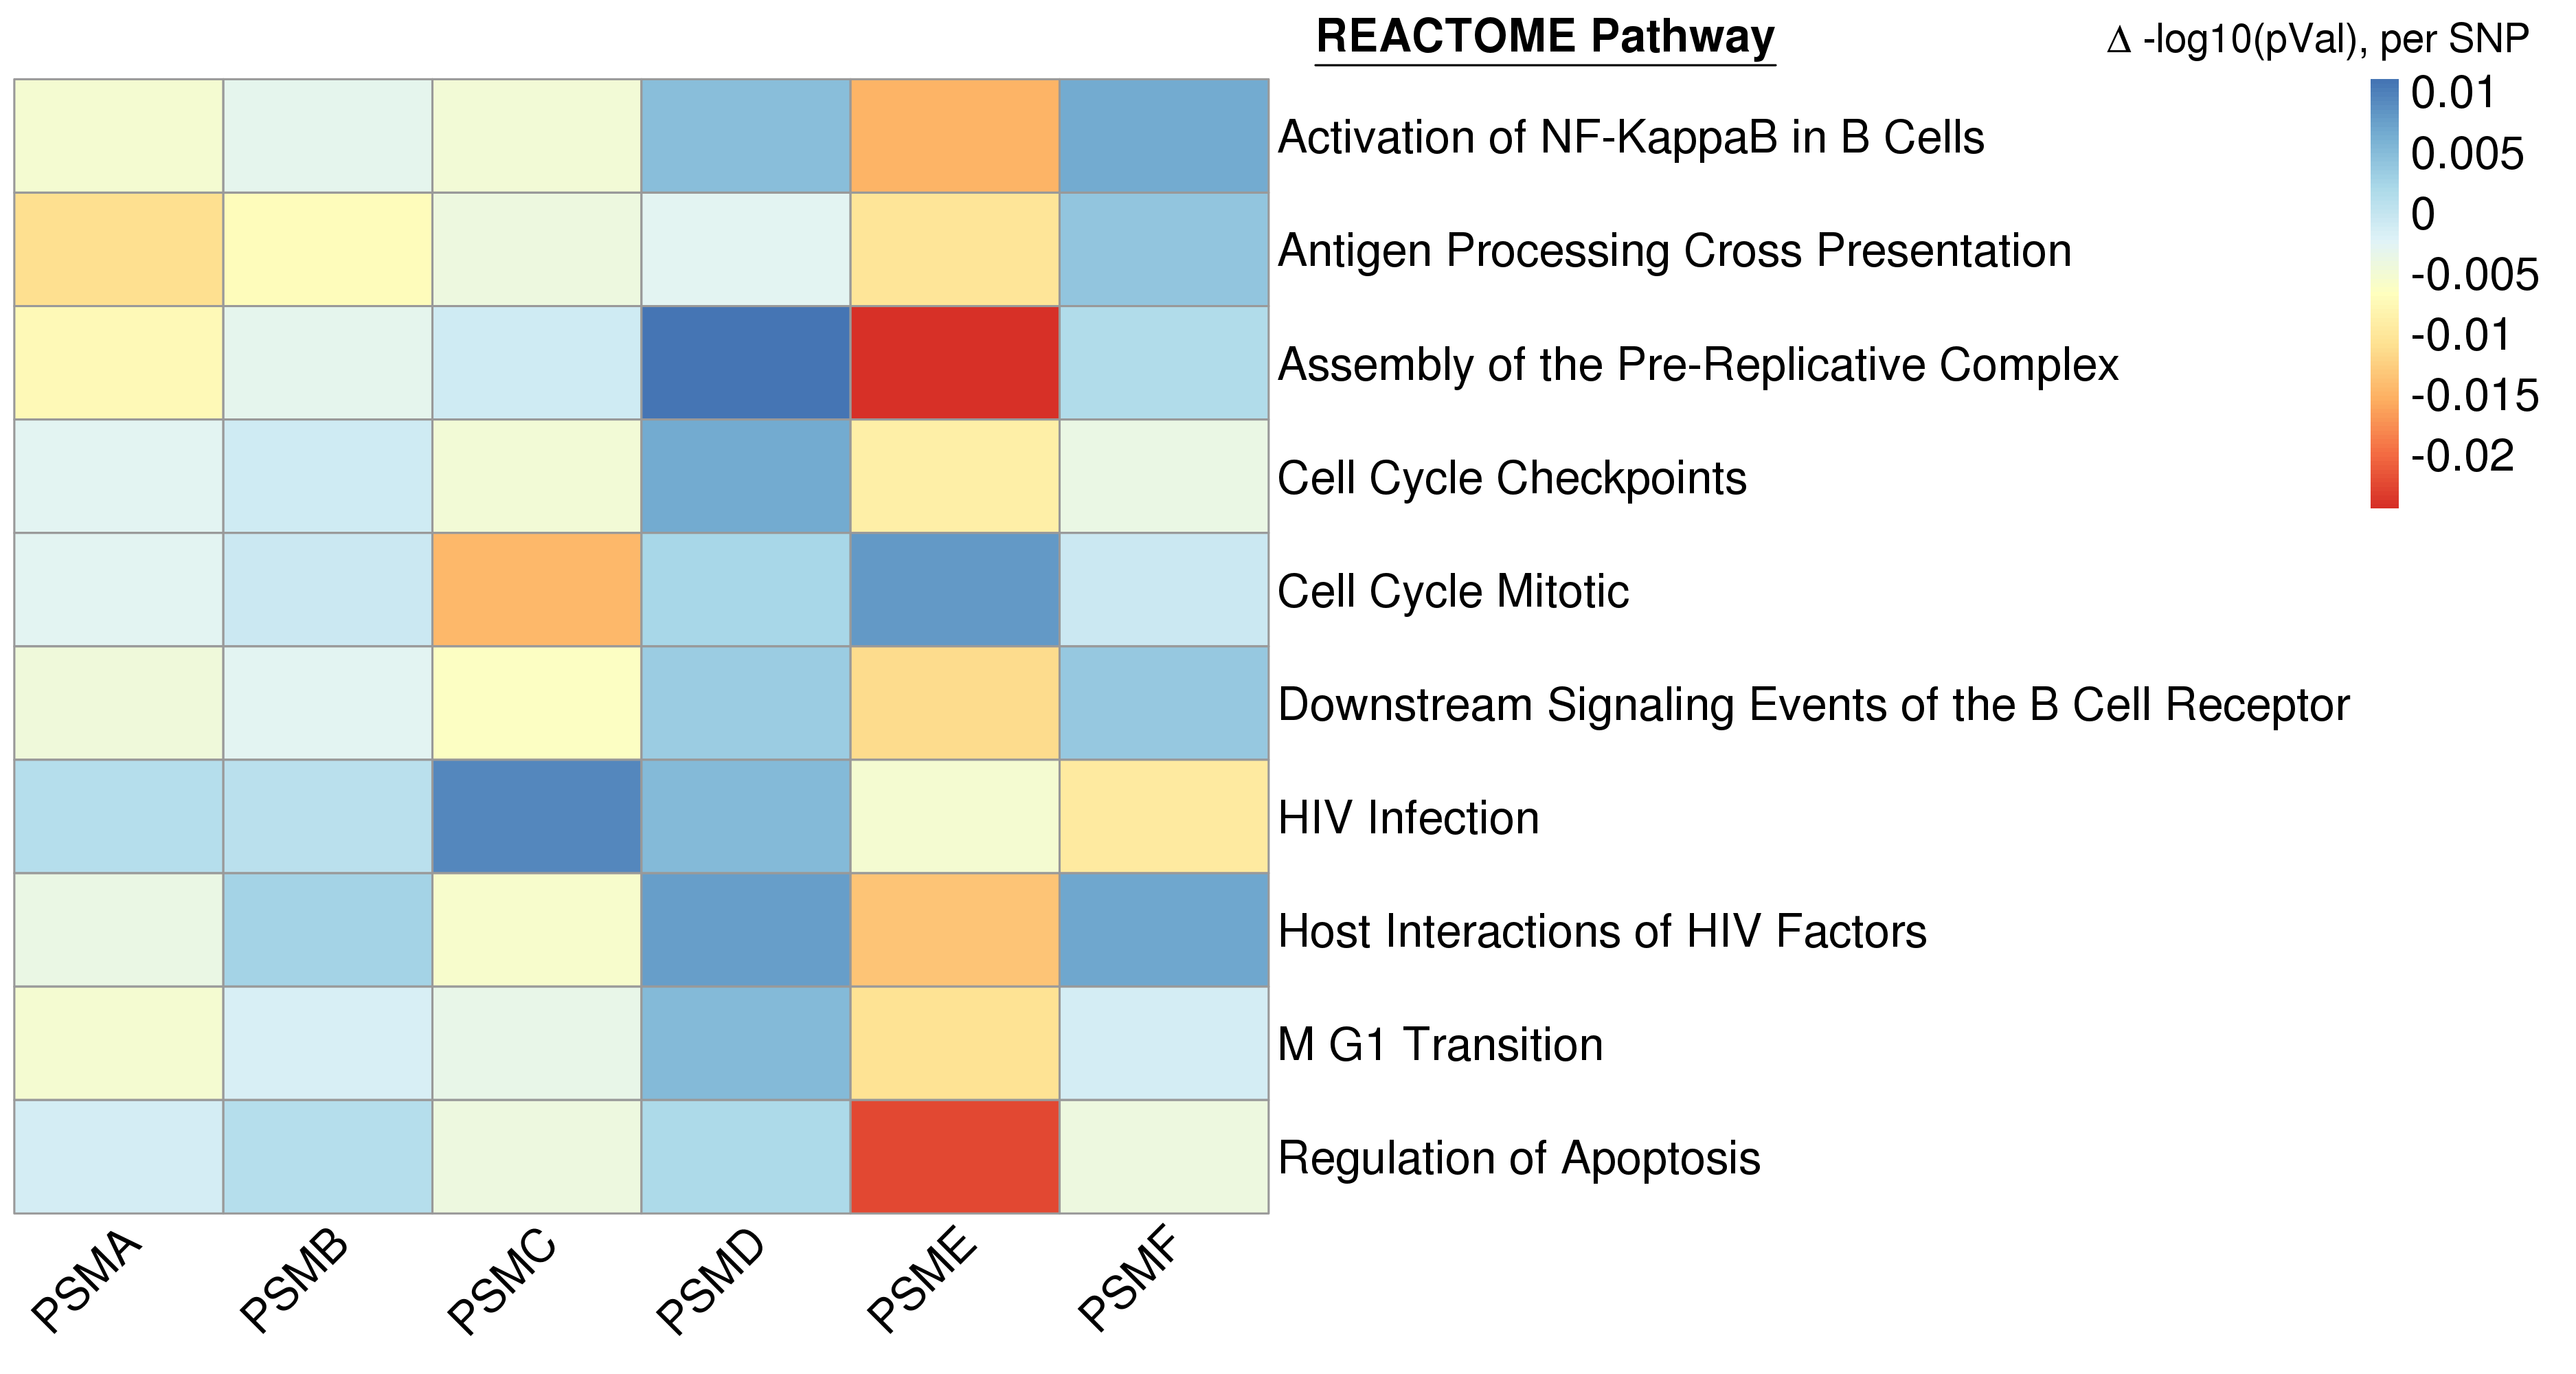
\includegraphics[width=\textwidth]{Images/Supp/InterPath_Supp_Figure_Proteaseome_Heatplots_BritRan4000_Loop_vs3.png}}
\subfigure[\textcolor{red}{Number of SNPs in each Proteasome Gene Family and REACTOME Pathway}]{
\setlength{\extrarowheight}{3pt}
 \hspace*{-1cm}
 \begin{tabular}{|cc|ccc|}
  \hline
\textbf{Gene Family} & \textbf{\# SNPs} & \textbf{REACTOME Pathway} & \textbf{\# SNPs} & \textbf{$\bm{P}$-Value}\\ [2pt]\hline
PSMA & 40 & Activation of NF-KappaB in B Cells & 756 & 2.28$\times10^{-1}$  \\[2pt]
PSMB & 91 & Antigen Processing Cross Presentation & 1104 & 2.48$\times10^{-5}$ \\[2pt]
PSMC & 29 & Assembly of the Pre-Replicative Complex & 507 & 1.84$\times10^{-2}$ \\[2pt]
PSMD & 101 & Cell Cycle Checkpoints & 1121 & 6.77$\times10^{-2}$ \\[2pt]
PSME & 25 & Cell Cycle Mitotic & 3304 & 2.34$\times10^{-1}$ \\[2pt]
 PSMF & 26 & Downstream Signaling Events of the B Cell Receptor & 1248 & 3.25$\times10^{-1}$ \\[2pt]
 & & HIV Infection & 2221 & 8.26$\times10^{-2}$ \\[2pt]
 & & Host Interactions of HIV Factors & 1541 & 1.55$\times10^{-2}$ \\[2pt]
 & & M G1 Transition & 697 & 3.02$\times10^{-1}$ \\[2pt]
 & & Regulation of Apoptosis & 906 & 2.98$\times10^{-2}$ \\[2pt]
  \hline
\end{tabular}}
\caption{\textbf{Results from applying a ``leave-one-out'' approach to MAPIT-R with proteasome gene families in body mass index (BMI) within 4,000 randomly subsampled individuals of British ancestry (\texttt{Brit.Ran4k}) in the UK Biobank.} \textbf{(a)} The heatmap shows the change in original MAPIT-R -$\log_{10}$ $p$-value for different REACTOME pathways when each proteasome gene family is removed one at a time in a `leave-one-out' manner. The x-axis shows each proteasome gene family and the y-axis lists each REACTOME pathway. Each column has been scaled by the number of SNPs present in the given gene family and, as a result, the heatmap specifically shows the -$\log_{10}$ $P$-value change per SNP. \textbf{(b)} The table shows the number of SNPs present in each proteasome gene family (left), as well as the number of SNPs present in each REACTOME pathway (right). The original MAPIT-R $P$-values are also shown for each pathway (right).}
\label{InterPath-Supp-Figure-Prot-Heatplots-BritRan4000}
\end{figure}
\clearpage

\begin{figure}[H]
\centering
\vspace*{-.5cm}
\subfigure[$\Delta$ in MAPIT-R -$\log_{10}$ $p$-value per SNP]{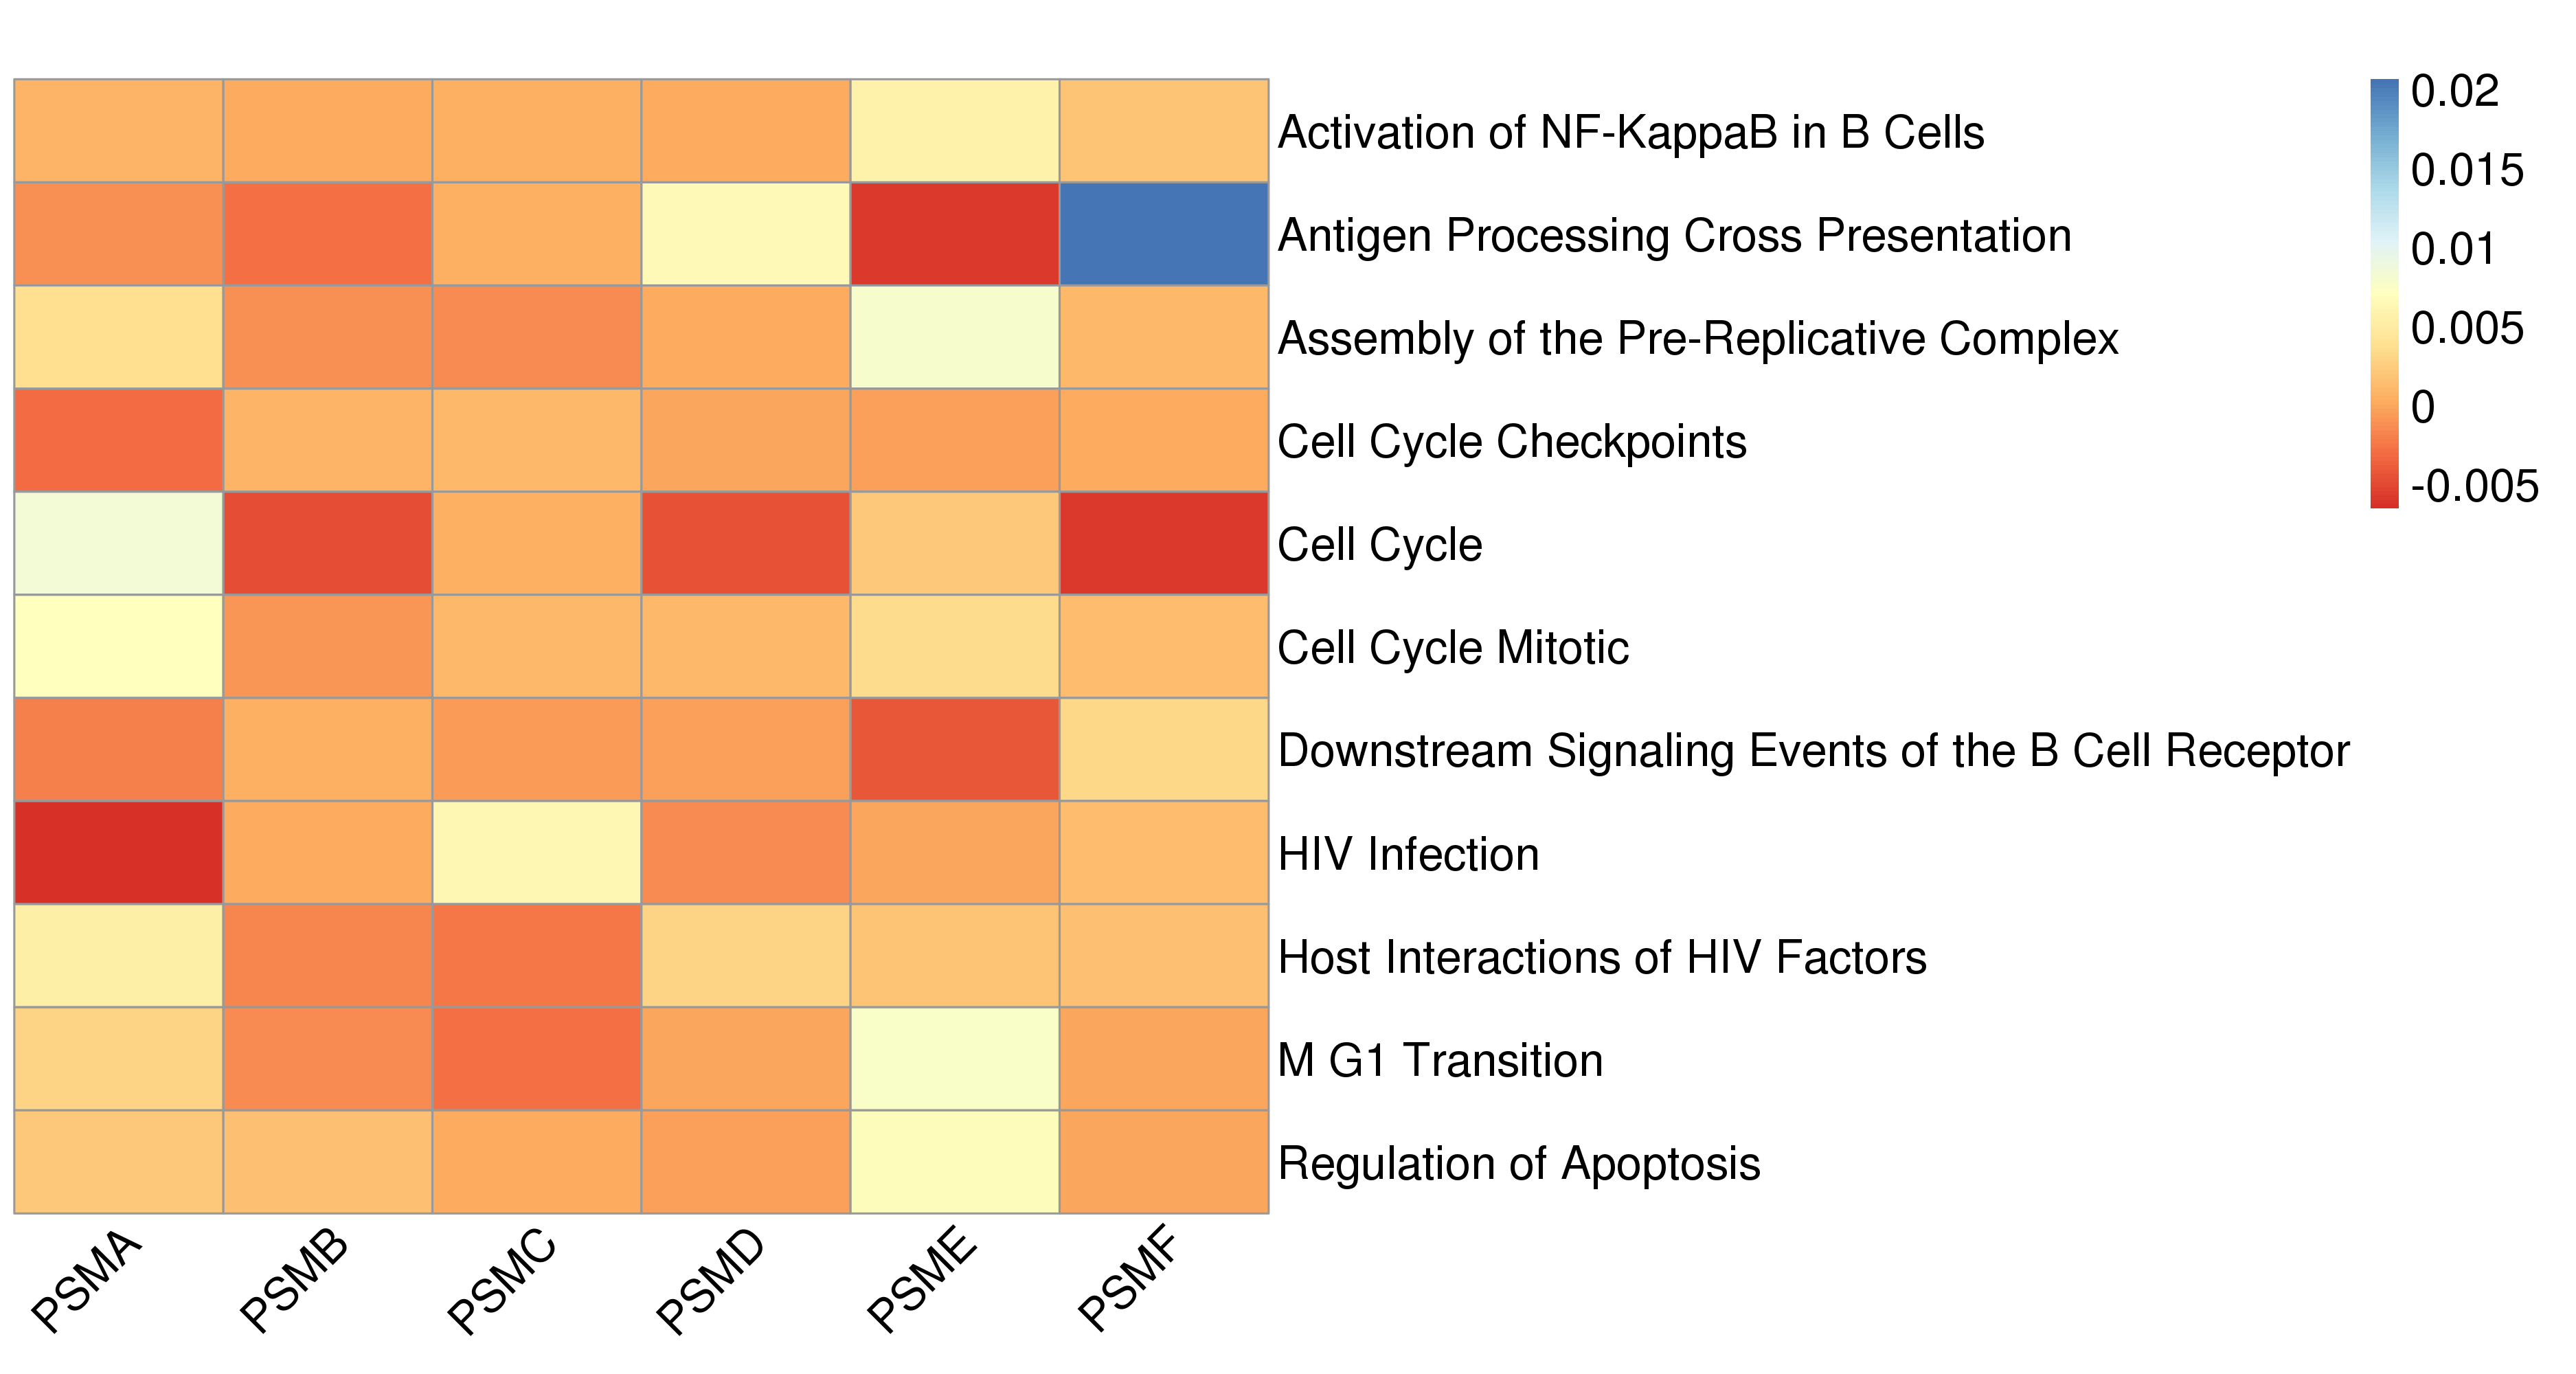
\includegraphics[width=\textwidth]{Images/Supp/InterPath_Supp_Figure_Proteaseome_Heatplots_Caribbean_Loop_vs3.png}}
\subfigure[\textcolor{red}{Number of SNPs in each Proteasome Gene Family and REACTOME Pathway}]{
\setlength{\extrarowheight}{3pt}
 \hspace*{-1cm}
 \begin{tabular}{|cc|ccc|}
  \hline
\textbf{Gene Family} & \textbf{\# SNPs} & \textbf{REACTOME Pathway} & \textbf{\# SNPs} & \textbf{$\bm{P}$-Value}\\ [2pt]\hline
PSMA & 18 & Activation of NF-KappaB in B Cells & 507 & 9.93$\times10^{-1}$   \\[2pt]
PSMB & 77 & Antigen Processing Cross Presentation & 871 & 5.15$\times10^{-2}$  \\[2pt]
PSMC & 21 & Assembly of the Pre-Replicative Complex & 357 & 7.25$\times10^{-1}$  \\[2pt]
PSMD & 69 & Cell Cycle Checkpoints & 736 & 8.83$\times10^{-1}$  \\[2pt]
PSME & 15 & Cell Cycle & 2711 & 2.51$\times10^{-1}$  \\[2pt]
PSMF & 16 & Cell Cycle Mitotic & 2111 & 7.98$\times10^{-1}$  \\[2pt]
 & & Downstream Signaling Events of the B Cell Receptor & 829 & 8.37$\times10^{-1}$  \\[2pt]
 & & HIV Infection & 1483 & 3.11$\times10^{-1}$  \\[2pt]
 & & Host Interactions of HIV Factors & 1055 & 6.68$\times10^{-1}$  \\[2pt]
 & & M G1 Transition & 500 & 6.37$\times10^{-1}$  \\[2pt]
 & & Regulation of Apoptosis & 615 & 9.42$\times10^{-1}$  \\[2pt]
  \hline
\end{tabular}}
\caption{\textbf{Results from applying a ``leave-one-out'' approach to MAPIT-R with proteasome gene families in body mass index (BMI) within the Caribbean cohort in the UK Biobank.} \textbf{(a)} The heatmap shows the change in original MAPIT-R -$\log_{10}$ $P$-value for different REACTOME pathways when each proteasome gene family is removed one at a time in a `leave-one-out' manner. The x-axis shows each proteasome gene family and the y-axis lists each REACTOME pathway. Each column has been scaled by the number of SNPs present in the given gene family and, as a result, the heatmap specifically shows the -$\log_{10}$ $P$-value change per SNP. \textbf{(b)} The table shows the number of SNPs present in each proteasome gene family (left), as well as the number of SNPs present in each REACTOME pathway (right). The original MAPIT-R $P$-values are also shown for each pathway (right).}
\label{InterPath-Supp-Figure-Prot-Heatplots-Caribbean}
\end{figure}
\clearpage

\begin{figure}[H]
\centering
\vspace*{-.5cm}
\subfigure[$\Delta$ in MAPIT-R -$\log_{10}$ $p$-value per SNP]{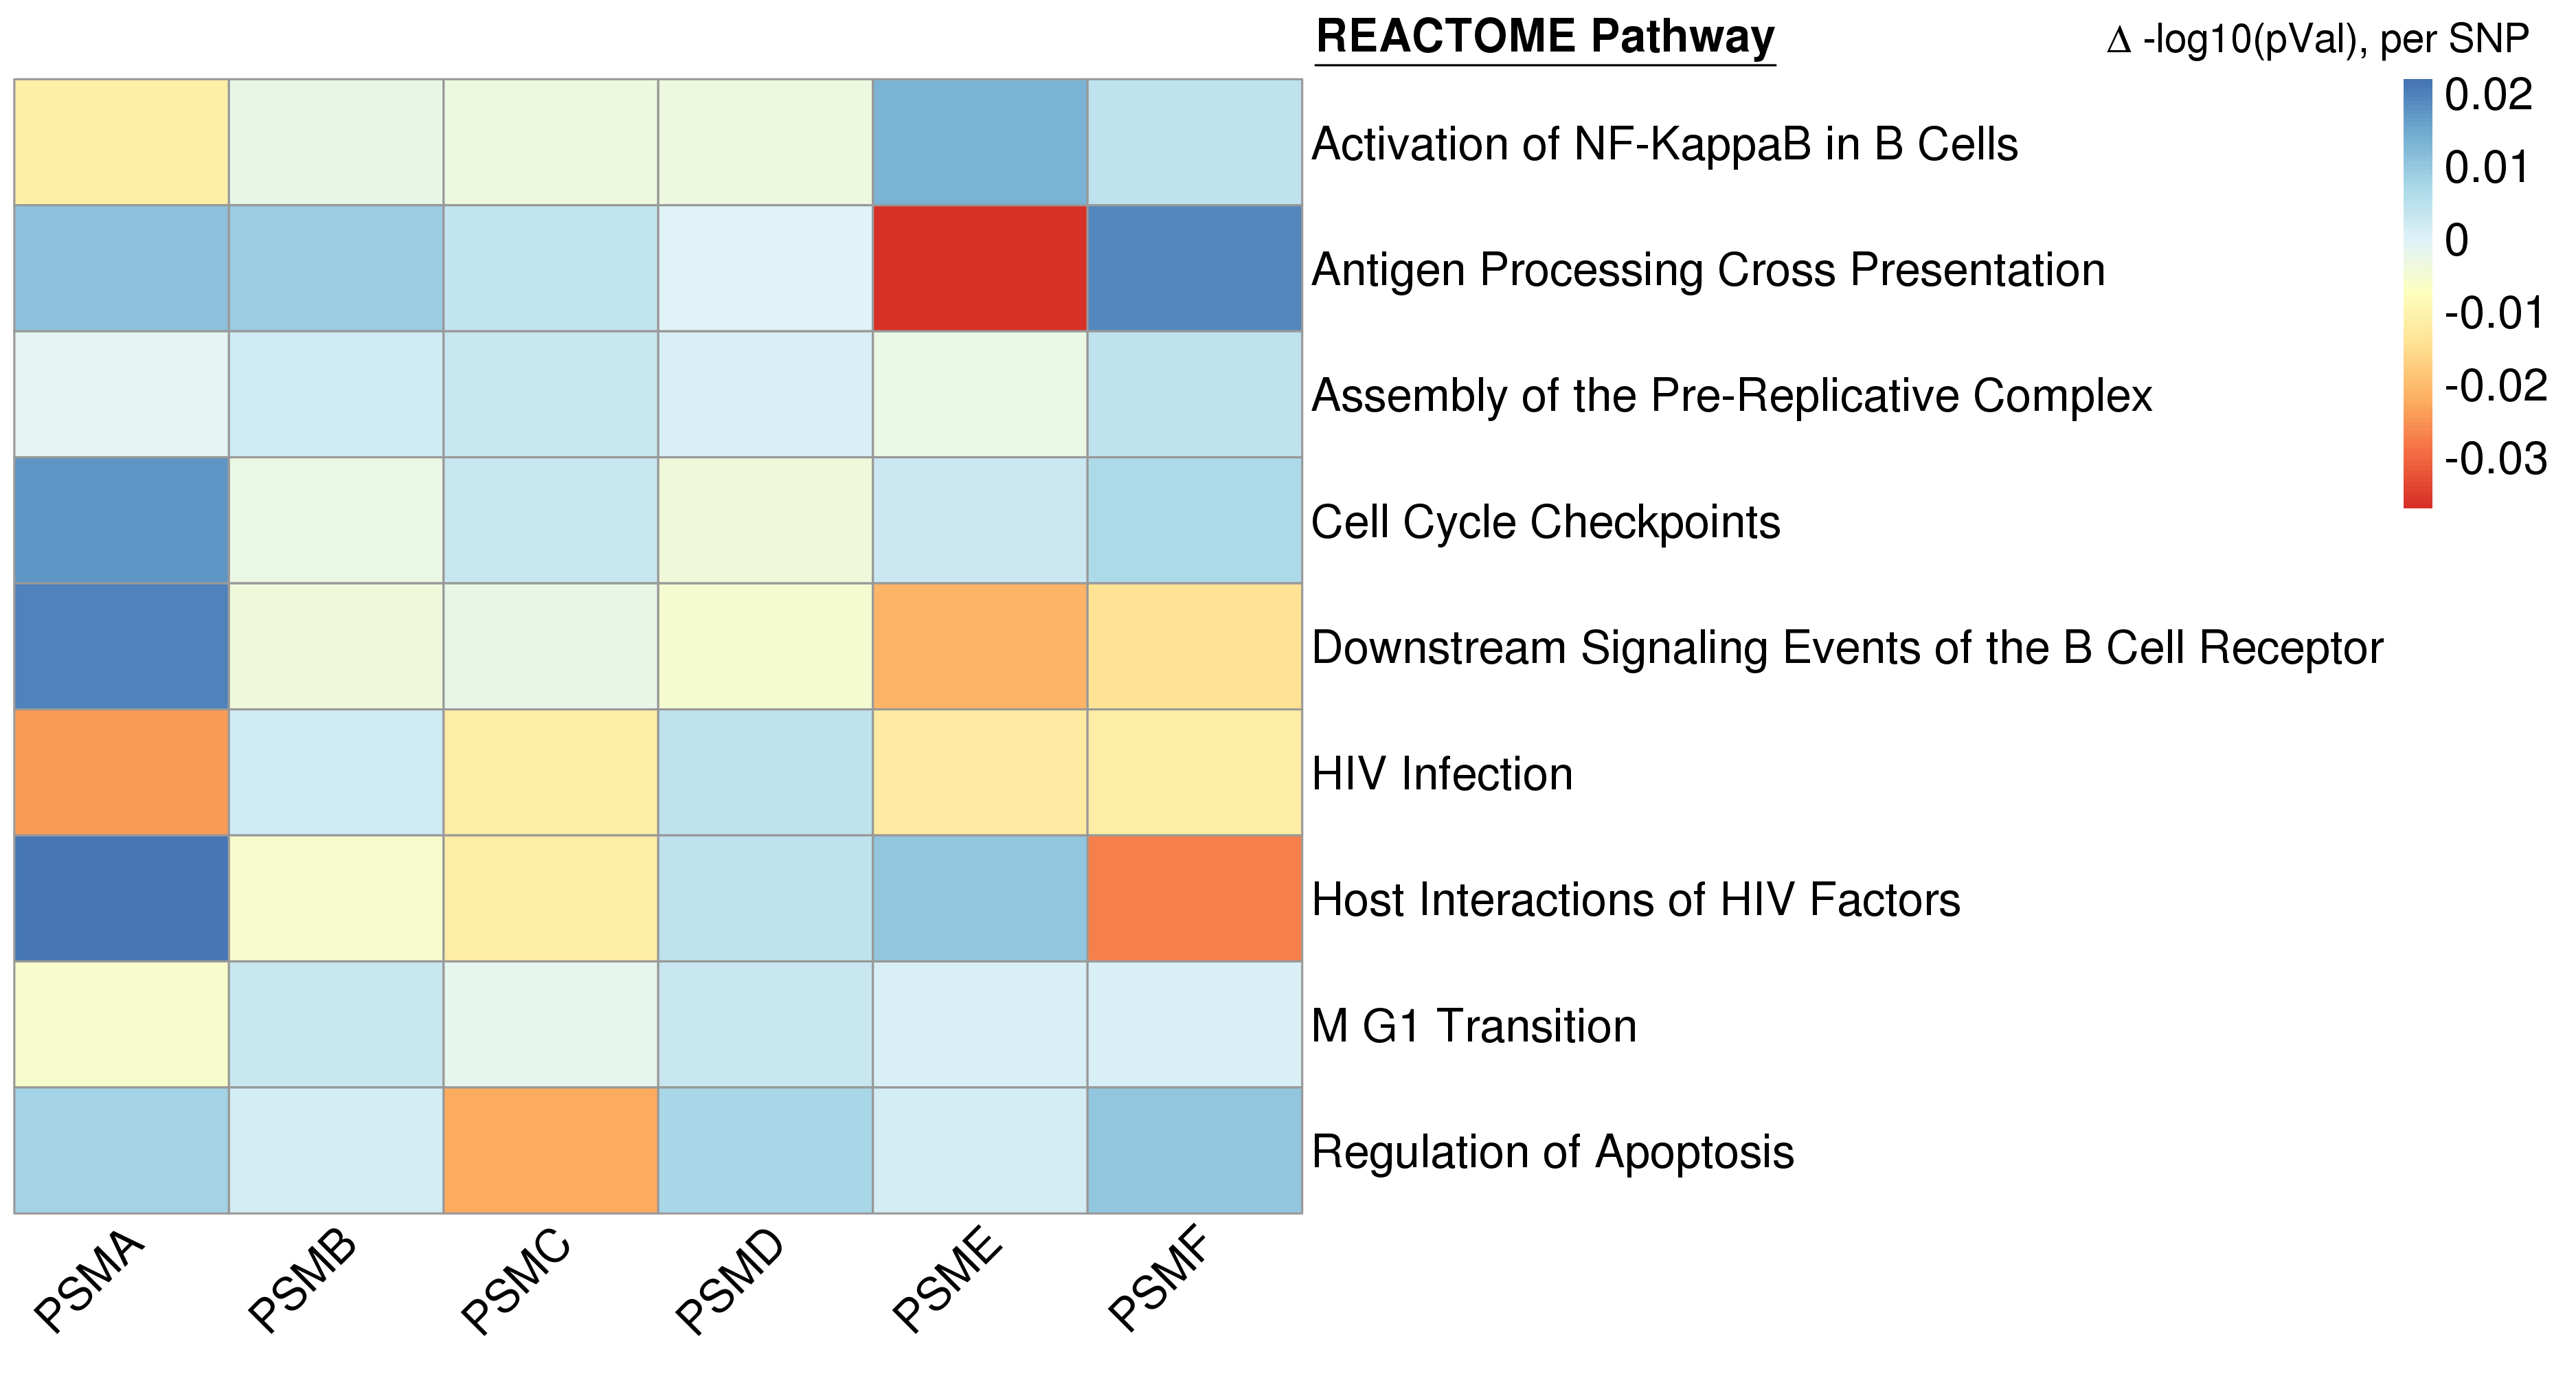
\includegraphics[width=\textwidth]{Images/Supp/InterPath_Supp_Figure_Proteaseome_Heatplots_Chinese_Loop_vs3.png}}
\subfigure[\textcolor{red}{Number of SNPs in each Proteasome Gene Family and REACTOME Pathway}]{
\setlength{\extrarowheight}{3pt}
 \hspace*{-1cm}
 \begin{tabular}{|cc|ccc|}
  \hline
\textbf{Gene Family} & \textbf{\# SNPs} & \textbf{REACTOME Pathway} & \textbf{\# SNPs} & \textbf{$\bm{P}$-Value}\\ [2pt]\hline
PSMA & 13 & Activation of NF-KappaB in B Cells & 433 & 5.27$\times10^{-1}$  \\[2pt]
PSMB & 74 & Antigen Processing Cross Presentation & 771 & 1.11$\times10^{-2}$ \\[2pt]
PSMC & 18 & Assembly of the Pre-Replicative Complex & 292 & 8.77$\times10^{-1}$ \\[2pt]
PSMD & 58 & Cell Cycle Checkpoints & 589 & 5.41$\times10^{-1}$  \\[2pt]
PSME & 12 & Downstream Signaling Events of the B Cell Receptor & 698 & 1.40$\times10^{-1}$ \\[2pt]
PSMF & 16 & HIV Infection & 1266 & 3.68$\times10^{-3}$ \\[2pt]
 & & Host Interactions of HIV Factors & 902 & 4.24$\times10^{-2}$\\[2pt]
 & & M G1 Transition & 400 & 8.20$\times10^{-1}$ \\[2pt]
 & & Regulation of Apoptosis & 527 & 2.26$\times10^{-2}$ \\[2pt]
  \hline
\end{tabular}}
\caption{\textbf{Results from applying a ``leave-one-out'' approach to MAPIT-R with proteasome gene families in body mass index (BMI) within the Chinese cohort in the UK Biobank.} \textbf{(a)} The heatmap shows the change in original MAPIT-R -$\log_{10}$ $P$-value for different REACTOME pathways when each proteasome gene family is removed one at a time in a `leave-one-out' manner. The x-axis shows each proteasome gene family and the y-axis lists each REACTOME pathway. Each column has been scaled by the number of SNPs present in the given gene family and, as a result, the heatmap specifically shows the -$\log_{10}$ $P$-value change per SNP. \textbf{(b)} The table shows the number of SNPs present in each proteasome gene family (left), as well as the number of SNPs present in each REACTOME pathway (right). The original MAPIT-R $P$-values are also shown for each pathway (right).}
\label{InterPath-Supp-Figure-Prot-Heatplots-Chinese}
\end{figure}
\clearpage

\begin{figure}[H]
\centering
\vspace*{-.5cm}
\subfigure[$\Delta$ in MAPIT-R -$\log_{10}$ $p$-value per SNP]{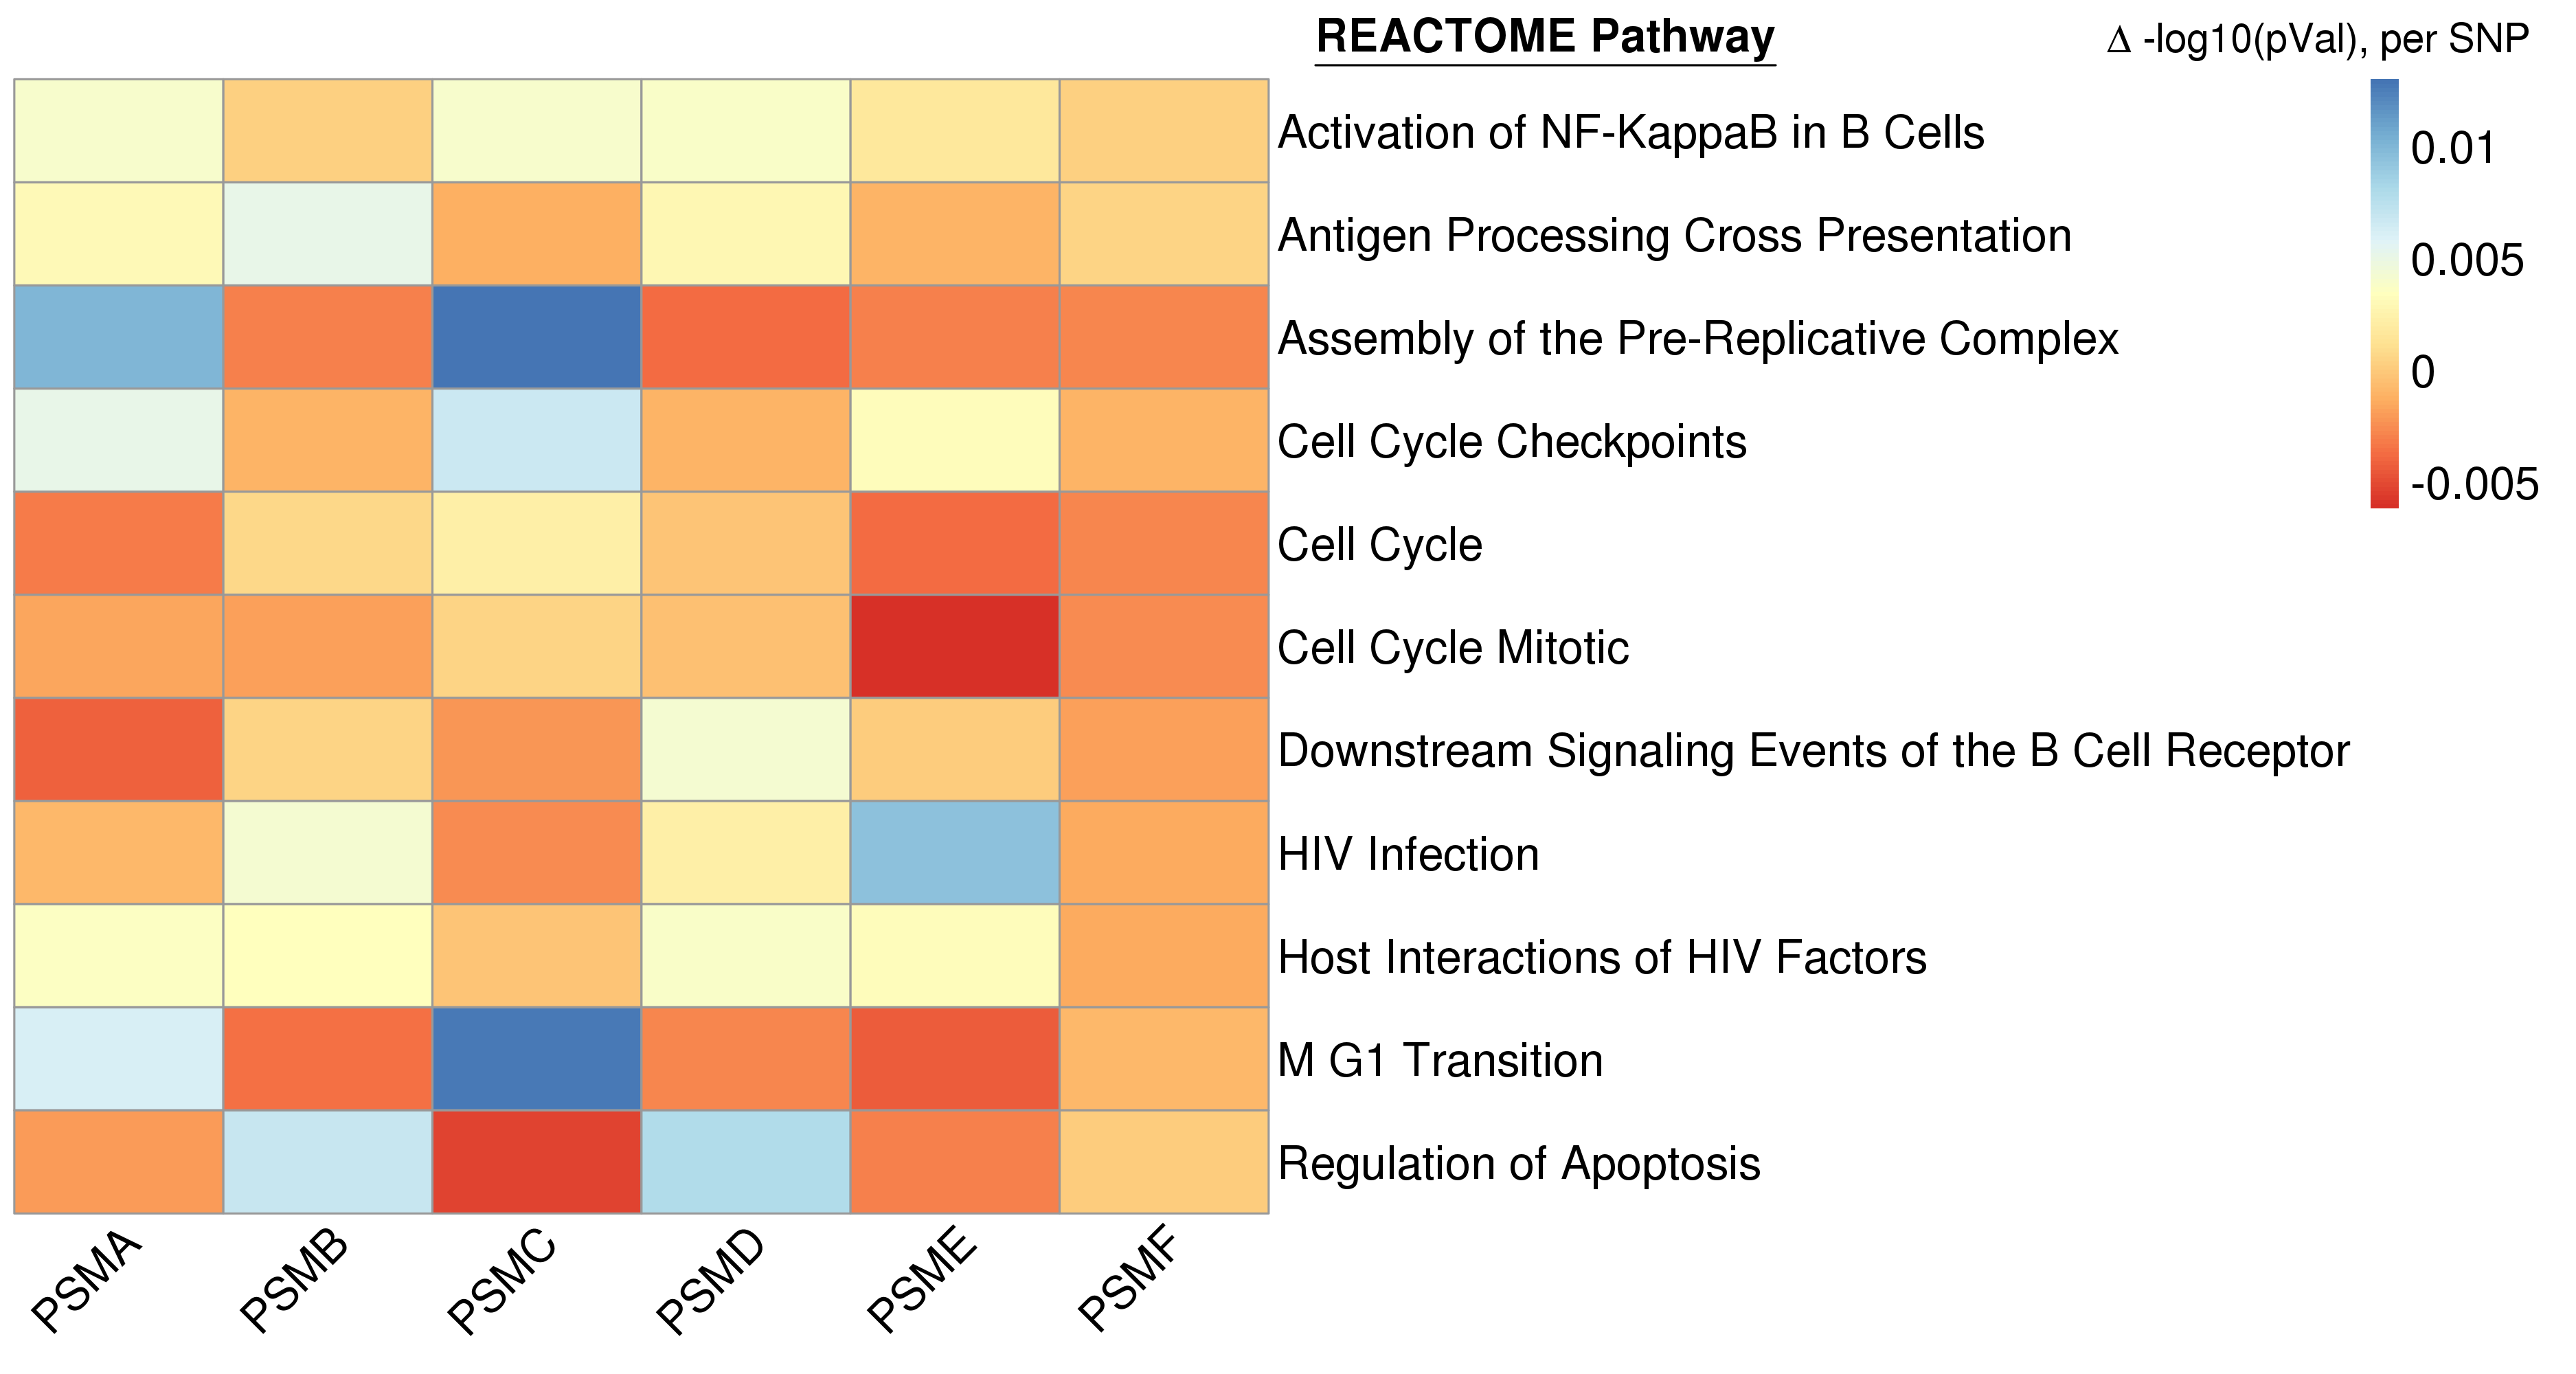
\includegraphics[width=\textwidth]{Images/Supp/InterPath_Supp_Figure_Proteaseome_Heatplots_Indian_Loop_vs3.png}}
\subfigure[\textcolor{red}{Number of SNPs in each Proteasome Gene Family and REACTOME Pathway}]{
\setlength{\extrarowheight}{3pt}
 \hspace*{-1cm}
 \begin{tabular}{|cc|ccc|}
  \hline
\textbf{Gene Family} & \textbf{\# SNPs} & \textbf{REACTOME Pathway} & \textbf{\# SNPs} & \textbf{$\bm{P}$-Value}\\ [2pt]\hline
PSMA & 29 & Activation of NF-KappaB in B Cells & 618 & 9.98$\times10^{-1}$  \\[2pt]
PSMB & 85 & Antigen Processing Cross Presentation & 977 & 4.48$\times10^{-1}$ \\[2pt]
PSMC & 25 & Assembly of the Pre-Replicative Complex & 427 & 5.02$\times10^{-1}$ \\[2pt]
PSMD & 78 & Cell Cycle Checkpoints & 909 & 8.04$\times10^{-1}$ \\[2pt]
PSME & 21 & Cell Cycle & 3361 & 1.87$\times10^{-1}$ \\[2pt]
PSMF & 21 & Cell Cycle Mitotic & 2656 & 2.32$\times10^{-1}$ \\[2pt]
 & & Downstream Signaling Events of the B Cell Receptor & 1037 & 5.53$\times10^{-1}$ \\[2pt]
 & & HIV Infection & 1836 & 9.80$\times10^{-2}$ \\[2pt]
 & & Host Interactions of HIV Factors & 1278 & 3.79$\times10^{-1}$ \\[2pt]
 & & M G1 Transition & 590 & 4.65$\times10^{-1}$ \\[2pt]
 & & Regulation of Apoptosis & 754 & 5.61$\times10^{-1}$\\[2pt]
  \hline
\end{tabular}}
\caption{\textbf{Results from applying a ``leave-one-out'' approach to MAPIT-R with proteasome gene families in body mass index (BMI) within the Indian cohort in the UK Biobank.} \textbf{(a)} The heatmap shows the change in original MAPIT-R -$\log_{10}$ $P$-value for different REACTOME pathways when each proteasome gene family is removed one at a time in a `leave-one-out' manner. The x-axis shows each proteasome gene family and the y-axis lists each REACTOME pathway. Each column has been scaled by the number of SNPs present in the given gene family and, as a result, the heatmap specifically shows the -$\log_{10}$ $P$-value change per SNP. \textbf{(b)} The table shows the number of SNPs present in each proteasome gene family (left), as well as the number of SNPs present in each REACTOME pathway (right). The original MAPIT-R $P$-values are also shown for each pathway (right).}
\label{InterPath-Supp-Figure-Prot-Heatplots-Indian}
\end{figure}
\clearpage

\begin{figure}[H]
\centering
\vspace*{-.5cm}
\subfigure[$\Delta$ in MAPIT-R -$\log_{10}$ $p$-value per SNP]{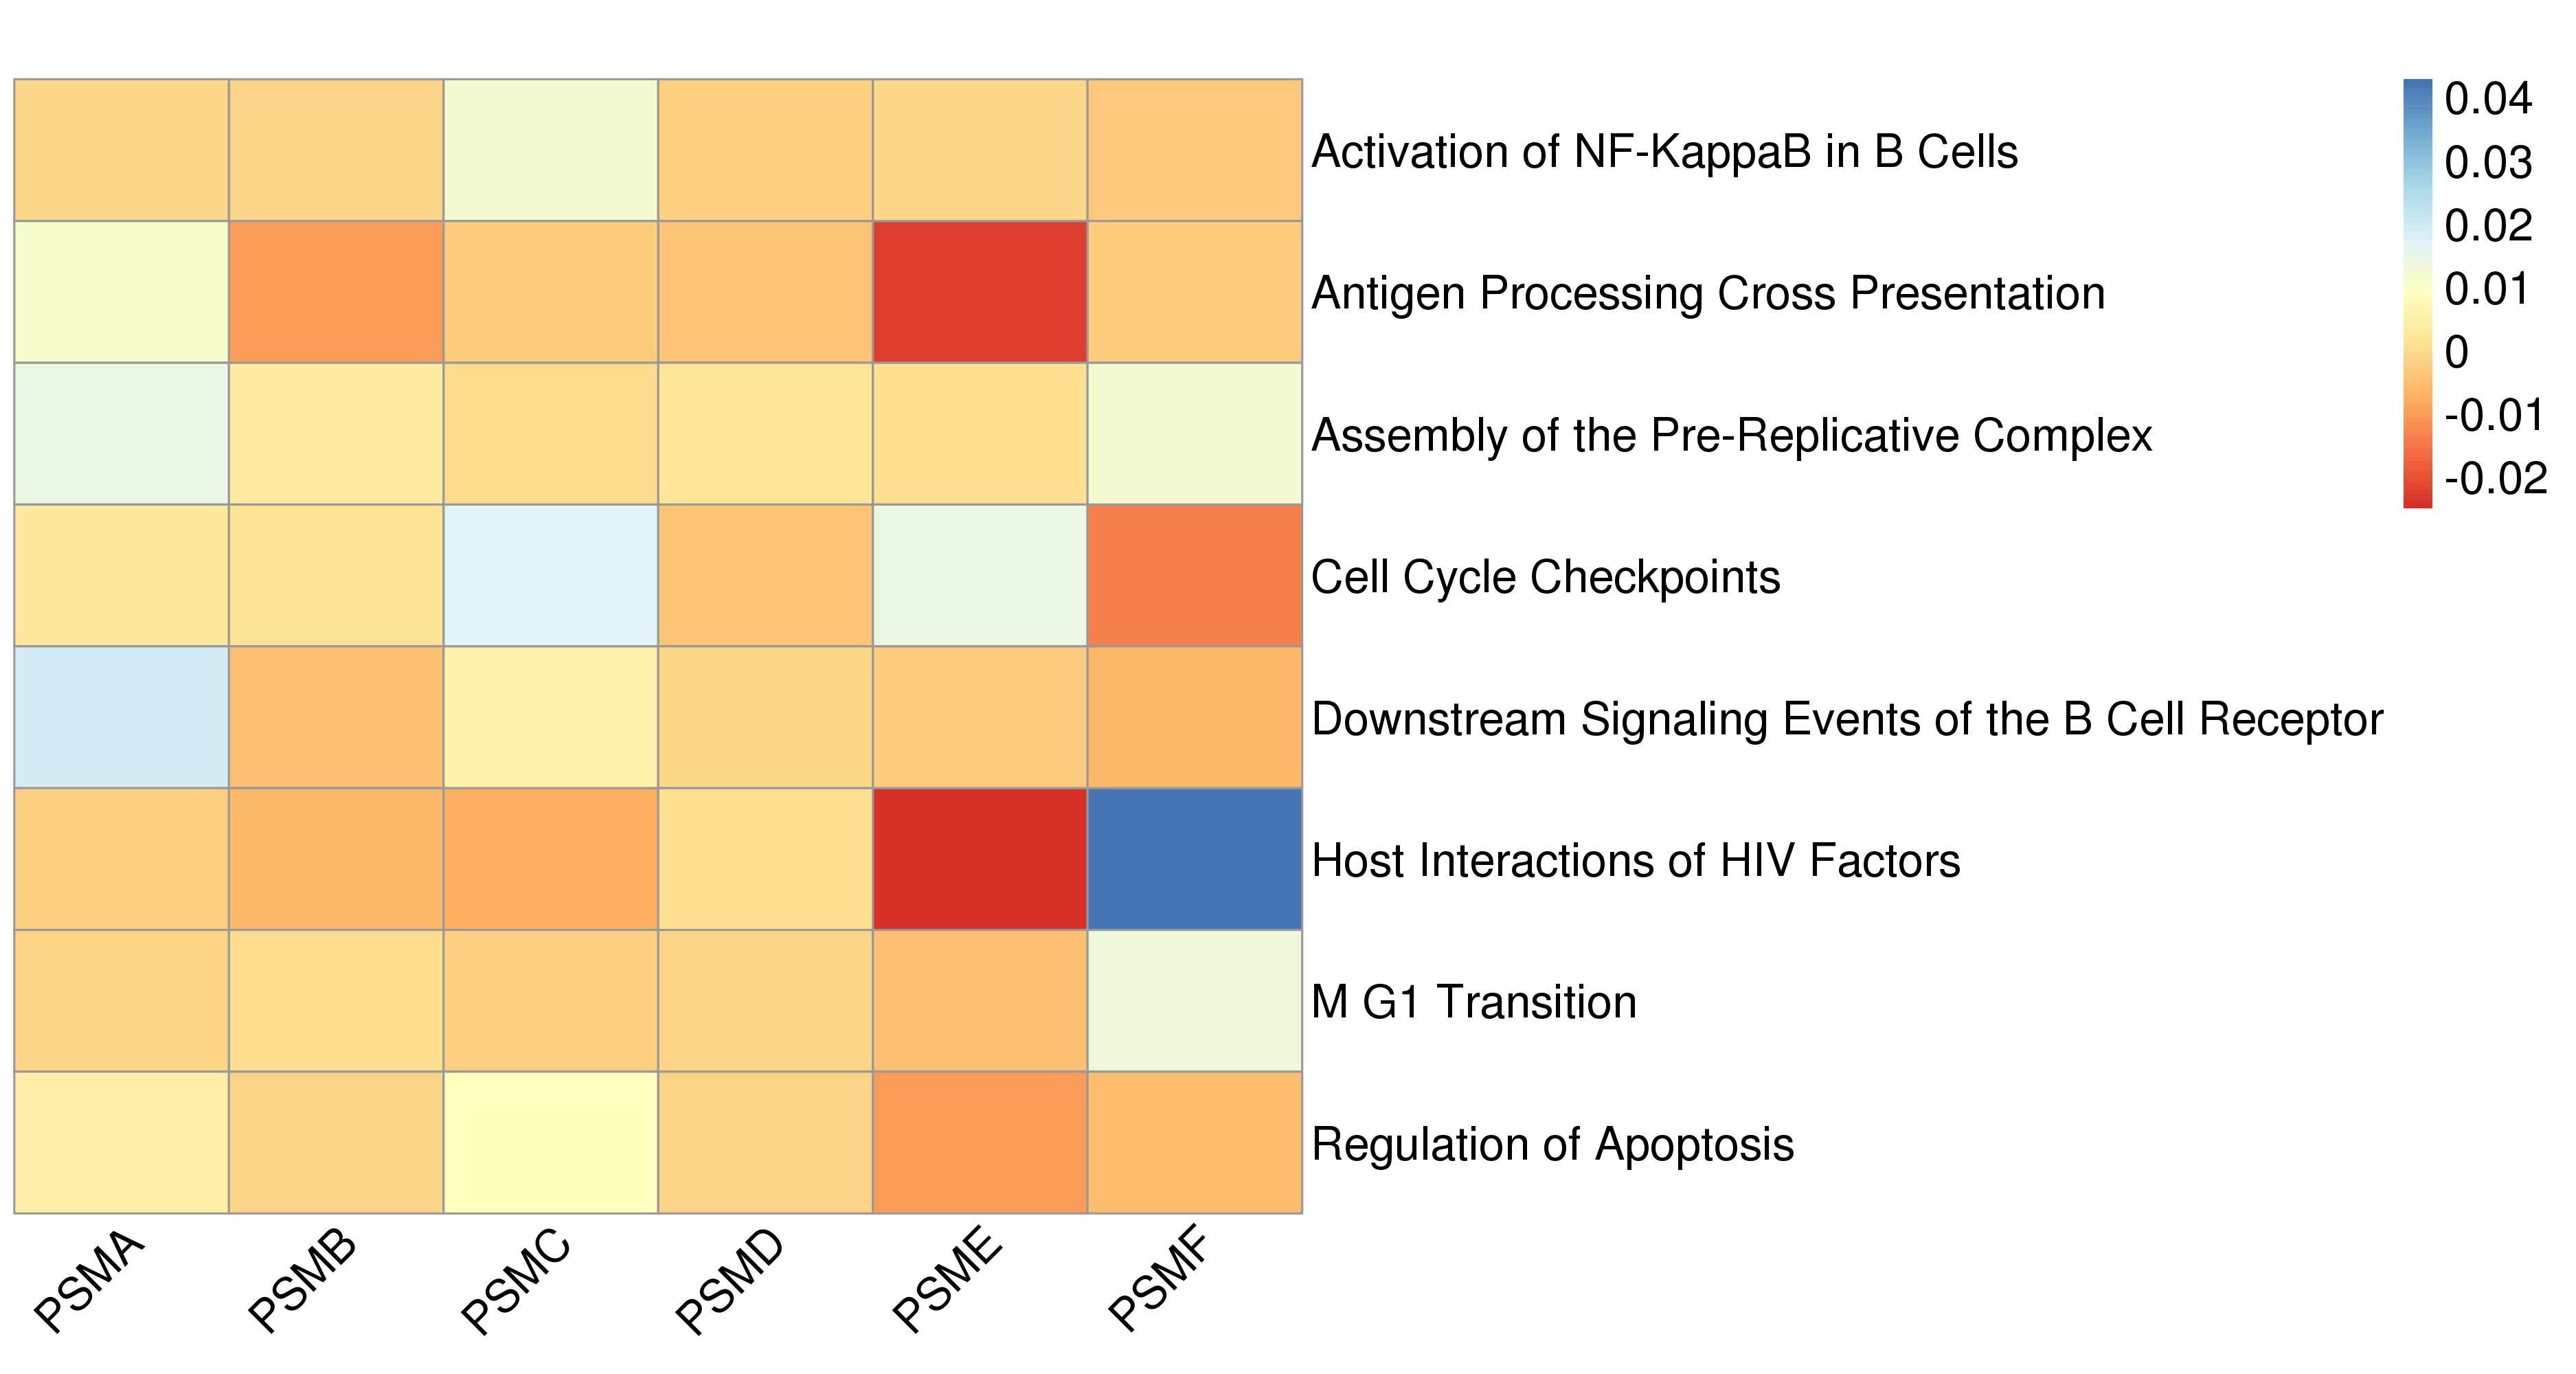
\includegraphics[width=\textwidth]{Images/Supp/InterPath_Supp_Figure_Proteaseome_Heatplots_Pakistani_Loop_vs3.png}}
\subfigure[\textcolor{red}{Number of SNPs in each Proteasome Gene Family and REACTOME Pathway}]{
\setlength{\extrarowheight}{3pt}
 \hspace*{-1cm}
 \begin{tabular}{|cc|ccc|}
  \hline
\textbf{Gene Family} & \textbf{\# SNPs} & \textbf{REACTOME Pathway} & \textbf{\# SNPs} & \textbf{$\bm{P}$-Value}\\ [2pt]\hline
PSMA & 30 & Activation of NF-KappaB in B Cells & 643 & 4.61$\times10^{-1}$  \\[2pt]
PSMB & 90 & Antigen Processing Cross Presentation & 1036 & 8.74$\times10^{-3}$ \\[2pt]
PSMC & 24 & Assembly of the Pre-Replicative Complex & 444 & 9.73$\times10^{-1}$ \\[2pt]
PSMD & 86 & Cell Cycle Checkpoints & 940 & 1.63$\times10^{-1}$ \\[2pt]
PSME & 21 & Downstream Signaling Events of the B Cell Receptor & 1073 & 6.57$\times10^{-2}$ \\[2pt]
PSMF & 22 & Host Interactions of HIV Factors & 1315 & 1.00$\times10^{-1}$ \\[2pt]
 & & M G1 Transition & 612 & 6.66$\times10^{-1}$ \\[2pt]
 & & Regulation of Apoptosis & 774 & 5.16$\times10^{-2}$ \\[2pt]
  \hline
\end{tabular}}
\caption{\textbf{Results from applying a ``leave-one-out'' approach to MAPIT-R with proteasome gene families in body mass index (BMI) within the Pakistani cohort in the UK Biobank.} \textbf{(a)} The heatmap shows the change in original MAPIT-R -$\log_{10}$ $P$-value for different REACTOME pathways when each proteasome gene family is removed one at a time in a `leave-one-out' manner. The x-axis shows each proteasome gene family and the y-axis lists each REACTOME pathway. Each column has been scaled by the number of SNPs present in the given gene family and, as a result, the heatmap specifically shows the -$\log_{10}$ $P$-value change per SNP. \textbf{(b)} The table shows the number of SNPs present in each proteasome gene family (left), as well as the number of SNPs present in each REACTOME pathway (right). The original MAPIT-R $P$-values are also shown for each pathway (right).}
\label{InterPath-Supp-Figure-Prot-Heatplots-Pakistani}
\end{figure}
\clearpage

%\addtocounter{figure}{1}
%\renewcommand{\thefigure}{\arabic{figure}}

%\setlength{\footskip}{2cm}
\begin{figure}[htbp]
\centering
\vspace*{-1cm}
%\vspace*{-1.75cm}
%\hspace*{-1cm}
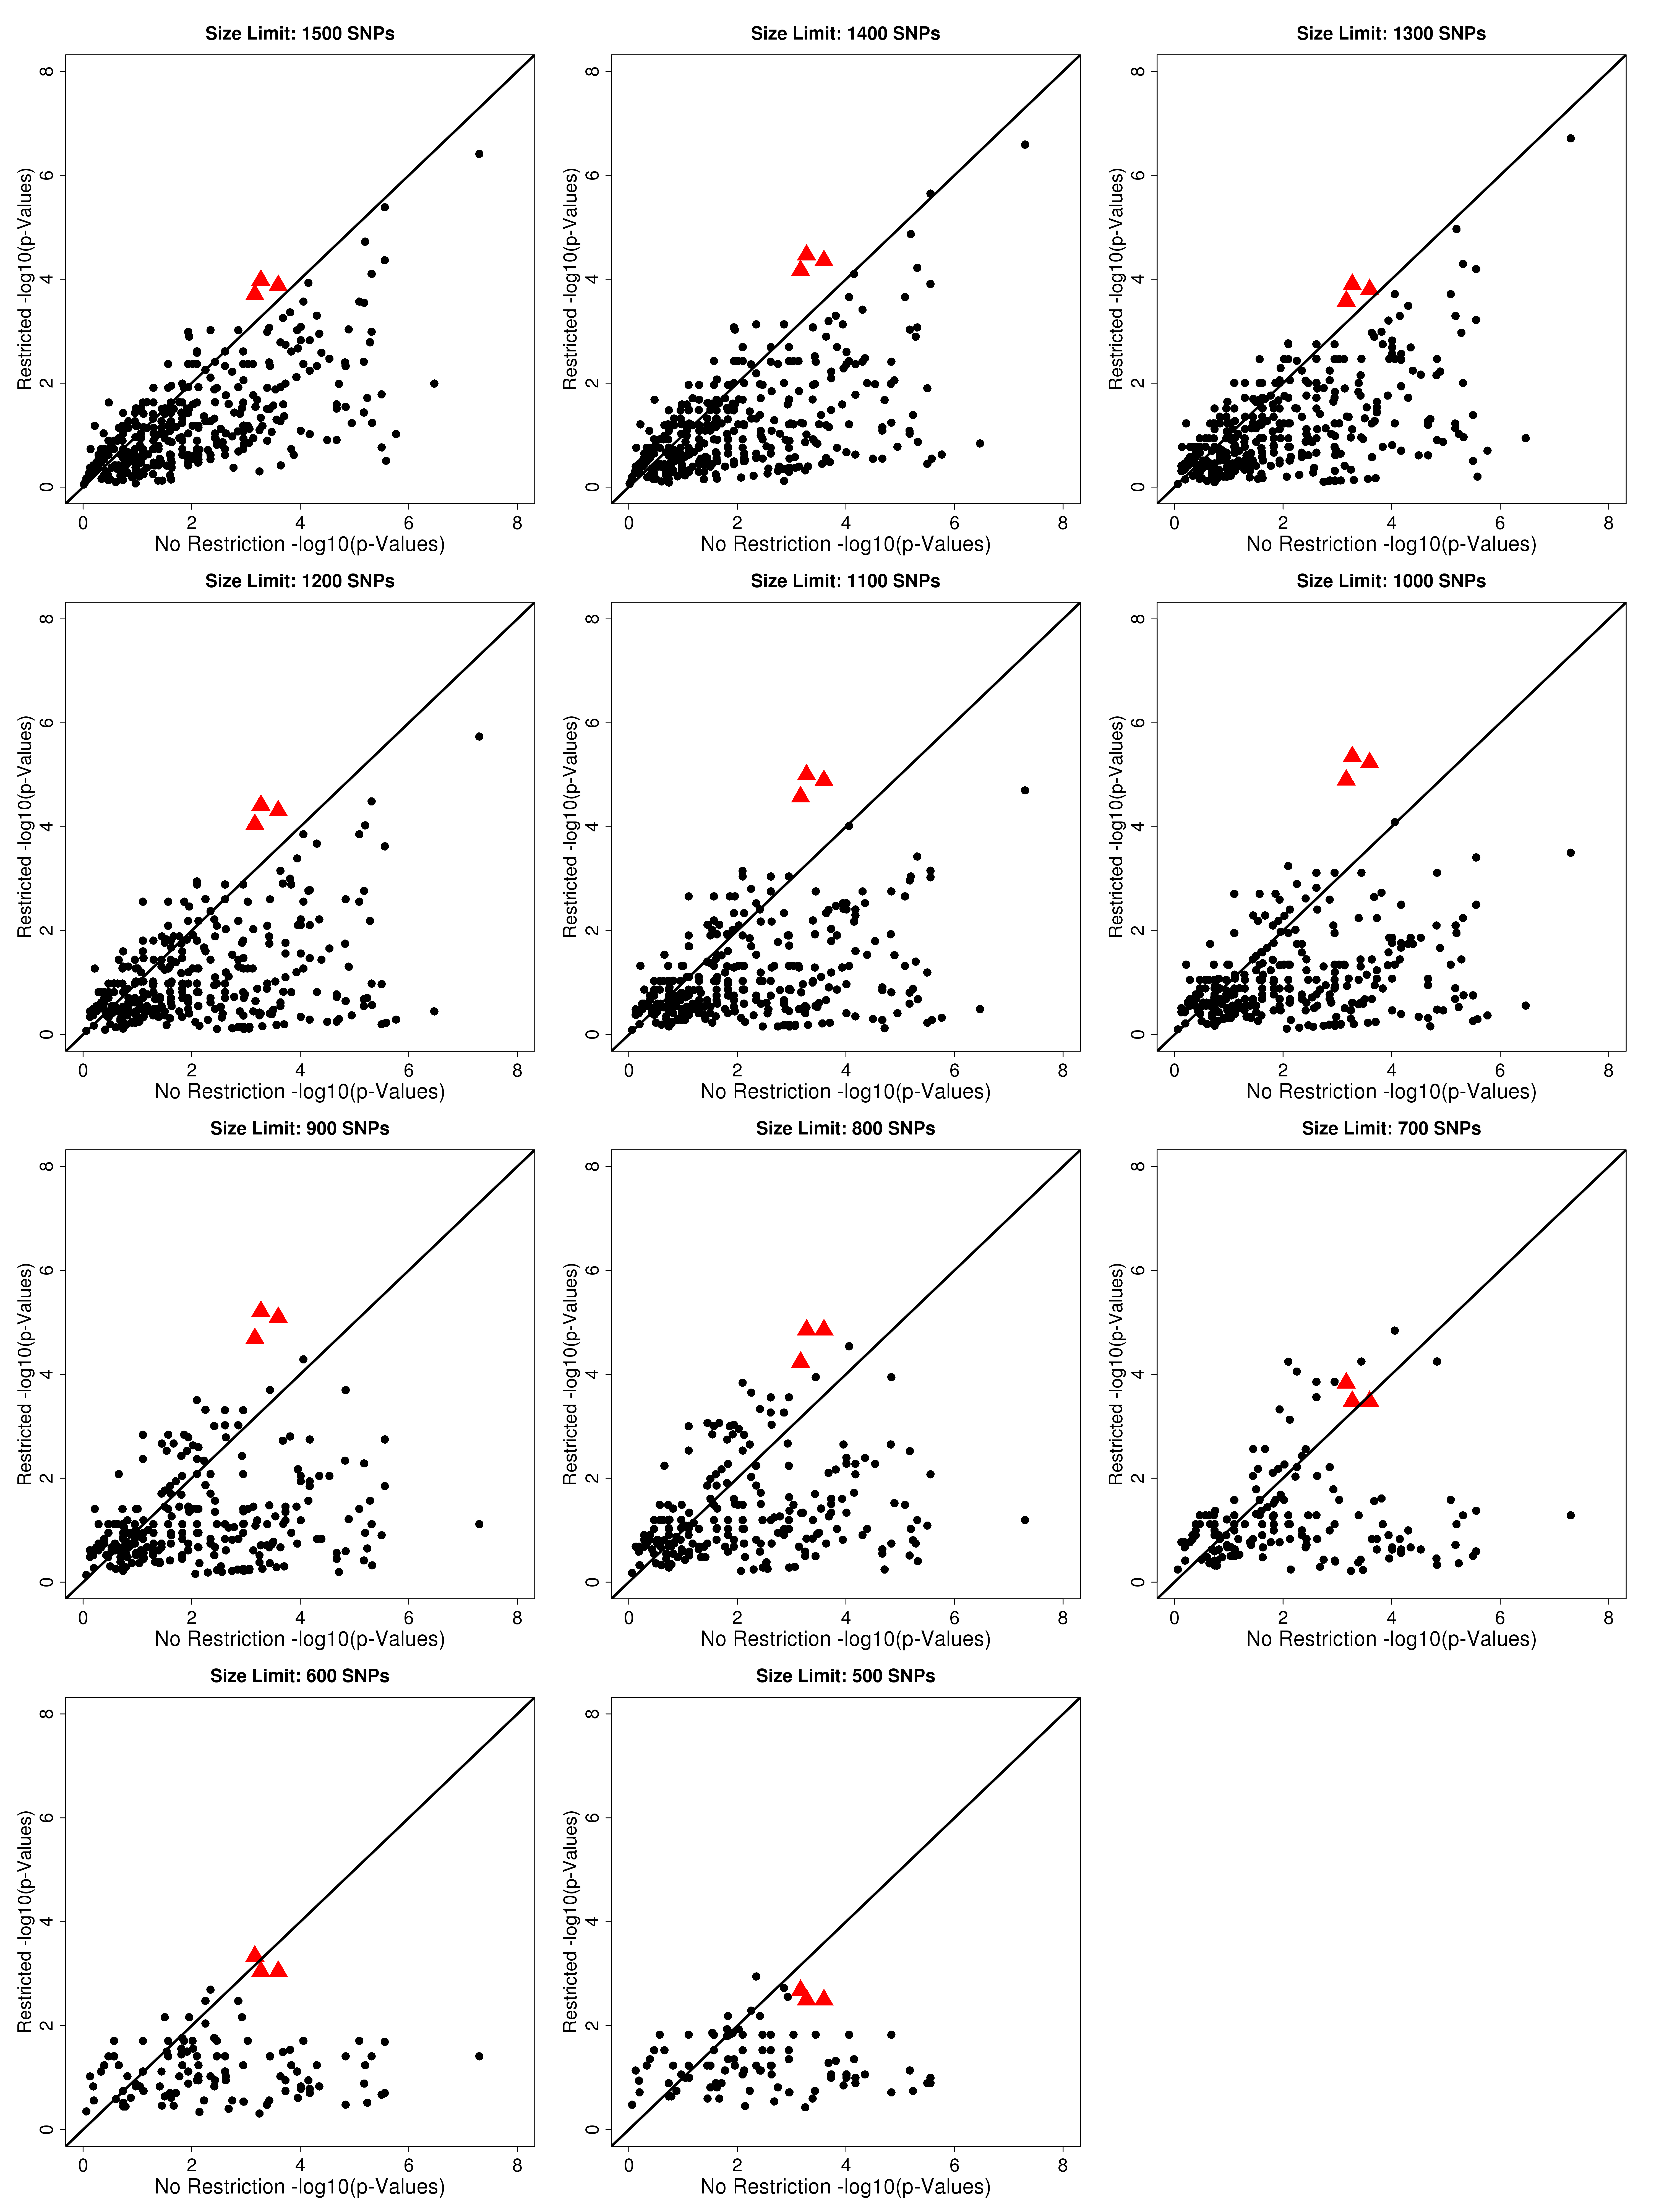
\includegraphics[width=0.9\textwidth]{Images/Supp/InterPath_Supp_Figure_Hypergemeotric_SizeThresholds_vs1.png}
\caption{\textbf{Impact of pathway size thresholds on hypergeometric enrichment analyses.} 
Here, we show multiple comparisons of size-restricted versus unrestricted hypergeometric 
enrichment analyses using incrementally decreasing pathway size thresholds. Size thresholds 
range from $T =$ 500 SNPs to 1,500 SNPs in 100-SNP increments. In each plot, the x-axis is the 
unrestricted hypergeometric $P$-value for each gene, while the y-axis is the size-restricted 
hypergeometric $P$-value for each gene. Red triangles represent results for each gene belonging 
to a proteasome gene family: {\emph{PSMA}}, {\emph{PSMB}}, {\emph{PSMC}}, {\emph{PSMD}}, 
{\emph{PSME}}, and {\emph{PSMF}}. Note that there are only three triangles since most proteasome 
genes are assigned to the same pathways.}
\label{InterPath-Supp-Figure-Hypergeoemtric-SizeThresholds}
\end{figure}
\clearpage
%\setlength{\footskip}{1cm}

%\addtocounter{figure}{-1}
%\begin{figure} [t!]
%  \caption{\textbf{Impact of pathway size thresholds on hypergeometric enrichment analyses}. The figure shows multiple comparisons of size-restricted hypergeometric enrichment analyses versus unrestricted hypergeometric enrichment analyses using incrementally decreasing pathway size thresholds. Size thresholds change from 1,500 SNPs to 500 SNPs in 100 SNP increments. In each plot the $x$-axis is the unrestricted hypergeometric $p$-value for each gene and the $y$-axis is the size-restricted hypergeometric $p$-value for each gene. Red triangles represent results for each gene belonging to a proteasome gene family ({\emph{PSMA}}, {\emph{PSMB}}, {\emph{PSMC}}, {\emph{PSMD}}, {\emph{PSME}}, and {\emph{PSMF}}). Note that there are only three triangles since most proteasome genes are assigned to the same pathways.}
%\label{InterPath-Supp-Figure-Hypergeoemtric-SizeThresholds-Caption}
%\end{figure}
%\clearpage

\section{Supplementary Tables}\label{Supplementary-Tables}

\setlength{\extrarowheight}{3pt}

\begin{table}[ht]
\centering
\begin{tabular}{|c|c|c|c|c|c|}
  \hline
\textbf{Subgroups} & \textbf{Ancestry} & \textbf{Individuals} & \textbf{SNPs} & \textbf{KEGG} & \textbf{REACTOME} \\
[2pt]\hline
 \multirow{6.5}{*}{\textbf{Original}} &African & 3111 & 374466 & 180 & 658 \\ [2pt]
& British (4k, Rep.~1) & 3848 & 600006 & 173 & 650 \\ [2pt]
& Caribbean & 3833 & 410017 & 181 & 661 \\ [2pt]
& Chinese & 1448 & 345221 & 153 & 626 \\ [2pt]
& Indian & 5077 & 505854 & 181 & 662 \\ [2pt]
& Pakistani & 1581 & 516806 & 141 & 596 \\ [2pt]\hline
\multirow{9.5}{*}{\textbf{British}} & British (4k, Rep.~2) & 3869 & 599381 & 173 & 650 \\[2pt] 
& British (4k, Rep.~3) & 3836 & 600654 & 173 & 649 \\ [2pt]
& British (4k, Rep.~4) & 3838 & 599829 & 173 & 650 \\ [2pt]
& British (4k, Rep.~5) & 3853 & 599442 & 173 & 650 \\ [2pt]
& British (10k, Rep.~1) & 9603 & 597298 & 186 & 669 \\ [2pt]
& British (10k, Rep.~2) & 9628 & 597577 & 186 & 669 \\ [2pt]
& British (10k, Rep.~3) & 9636 & 597486 & 186 & 669 \\ [2pt]
& British (10k, Rep.~4) & 9593 & 597369 & 186 & 669 \\ [2pt]
& British (10k, Rep.~5) & 9596 & 597507 & 186 & 669 \\ [2pt]
  \hline
\end{tabular}
\caption{\textbf{Tabulation of the number of subgroups, individuals, SNPs, and pathways analyzed in this study}. Here, the category ``original'' subgroups refers to the multiple global human ancestries from the UK Biobank that were initially analyzed at the beginning of this study, while the ``British replicates'' refers specifically to the different subgroups that were created by taking random independent subsamples of the full British cohort in the UK Biobank. The number of individuals and SNPs in the second and third columns are those post quality-control (see Supplementary Note), and the number of KEGG and REACTOME pathways analyzed within each subgroup are shown in the fourth and fifth columns. Note that for the ``British replicate'' subgroups, each dataset initially began with either 4,000 or 10,000 individuals before quality-control.}
\label{InterPath-Supp-Table-UKBPopStats}
\end{table}

%Irish & 11575 & 588324 & 186 & 671 \\ 

%\textbf{Supplementary Tables 2a-d.} \textbf{Lists of New \bmass{} Multivariate Associations, per Dataset}. \\ Attached Excel sheets list new \bmass{} associations for each dataset analyzed.
%\bigskip \bigskip

\begin{table}[H]
\caption{\textbf{List of MAPIT-R significant pathways genome-wide for standing height and body mass index (BMI) across the different ancestry-specific subgroups in the UK Biobank.} Here, subgroups in the UK Biobank included individuals based on their self-identified ancestries: ``African'', ``British'', ``Caribbean'', ``Chinese'', ``Indian'', and ``Pakistani'', respectively. Phenotype and pathway database combinations include: (\textit{i}) KEGG+Height, (\textit{ii}) KEGG+BMI, (\textit{iii}) REACTOME+Height, and (\textit{iv}) REACTOME+BMI. Genome-wide significance was determined by using Bonferroni-corrected $p$-value thresholds based on the number of pathways tested in each database-phenotype-subgroup combination with significance value $\alpha = 0.05$ (see Supplementary Table \ref{InterPath-Supp-Table-UKBPopStats}). (XLSX)}
\label{InterPath-Supp-Table-TopPathways-AllPaths-AllPhenos}
\end{table}

\clearpage

\begin{landscape}

\setlength{\extrarowheight}{3pt}

\begin{table}[ht]
\centering
\vspace*{-1.5cm}
\hspace*{-2em}
\begin{tabular}{|c|c|c|ccc|cc|cc|}
  \hline
& & & \multicolumn{3}{c|}{\textbf{$\bm{\alpha =}$ Bonferroni Correction}} & \multicolumn{2}{c|}{\textbf{$\bm{\alpha = 0.001}$ Thresh.}} & \multicolumn{2}{c|}{\textbf{$\bm{\alpha = 0.01}$ Thresh.}}\\
\hline
\textbf{Database (Trait)} & \textbf{Subgroup} & \textbf{\# Pathways} & \textbf{Thresh.} & \textbf{\# FPs} & \textbf{FDR (\%)} & \textbf{\# FPs} & \textbf{FDR (\%)} &  \textbf{\# FPs} & \textbf{FDR (\%)} \\ 
  \hline
\multirow{6.5}{*}{\textbf{KEGG (Height)}} & African & 1800 & 2.78$\times10^{-4}$ & 0 & 0.000  & 1 & 0.056 & 10 & 0.556 \\ 
  & British (4k) & 1730 & 2.89$\times10^{-4}$ & 0 & 0.000 & 0 & 0.000 & 13 & 0.751 \\ 
  & Caribbean & 1810 & 2.76$\times10^{-4}$ & 1 & 0.055 & 1 & 0.055 & 5 & 0.276 \\ 
  & Chinese & 1530 & 3.27$\times10^{-4}$ & 0 & 0.000 & 3 & 0.196 & 24 & 1.569 \\ 
  & Indian & 1810 & 2.76$\times10^{-4}$ & 1 & 0.055 & 1 & 0.055 & 20 & 1.105 \\ 
  & Pakistani & 1410 & 3.55$\times10^{-4}$ & 0 & 0.000 & 2 & 0.142 & 17 & 1.206 \\ 
  \hline
\multirow{6.5}{*}{\textbf{KEGG (BMI)}} & African & 1800 & 2.778$\times10^{-4}$ & 0 & 0.000 & 1 & 0.056 & 16 & 0.889 \\
 & Caribbean & 1810 & 2.762$\times10^{-4}$ & 0 & 0.000 & 1 & 0.055 & 25 & 1.381 \\ 
 & Chinese & 1530 & 3.268$\times10^{-4}$ & 0 & 0.000 & 1 & 0.065 & 24 & 1.569 \\ 
 & Indian & 1810 & 2.762$\times10^{-4}$ & 1 & 0.055 & 2 & 0.110 & 20 & 1.105 \\ 
 & Irish & 1860 & 2.688$\times10^{-4}$ & 0 & 0.000 & 0 & 0.000 & 14 & 0.753 \\ 
 & Pakistani & 1410 & 3.546$\times10^{-4}$ & 0 & 0.000 & 2 & 0.142 & 15 & 1.064 \\ 
  \hline
\multirow{6.5}{*}{\textbf{REACTOME (Height)}} & African & 6580 & 7.599$\times10^{-5}$ & 0 & 0.000 & 6 & 0.091 & 47 & 0.714 \\ 
 & Caribbean & 6610 & 7.564$\times10^{-5}$ & 0 & 0.000 & 2 & 0.030 & 22 & 0.333 \\ 
 & Chinese & 6260 & 7.987$\times10^{-5}$ & 0 & 0.000 & 13 & 0.208 & 85 & 1.358 \\ 
 & Indian & 6620 & 7.553$\times10^{-5}$ & 1 & 0.015 & 5 & 0.076 & 90 & 1.360 \\ 
 & Irish & 6710 & 7.452$\times10^{-5}$ & 0 & 0.000 & 1 & 0.015 & 55 & 0.820 \\
 & Pakistani & 5960 & 8.389$\times10^{-5}$ & 0 & 0.000 & 3 & 0.050 & 63 & 1.057 \\
\hline 
\multirow{6.5}{*}{\textbf{REACTOME (BMI)}} & African & 6580 & 7.60$\times10^{-5}$ & 1 & 0.015 & 4 & 0.061 & 39 & 0.593 \\
 & British (4k) & 6490 & 7.70$\times10^{-5}$ & 1 & 0.015 & 4 & 0.062 & 52 & 0.801 \\
 & Caribbean & 6610 & 7.56$\times10^{-5}$ & 0 & 0.000 & 13 & 0.197 & 97 & 1.467 \\
 & Chinese & 6260 & 7.99$\times10^{-5}$ & 0 & 0.000 & 6 & 0.096 & 49 & 0.783 \\
 & Indian & 6620 & 7.55$\times10^{-5}$ & 0 & 0.000 & 3 & 0.045 & 66 & 0.997 \\
 & Pakistani & 5960 & 8.39$\times10^{-5}$ & 0 & 0.000 & 4 & 0.067 & 45 & 0.755 \\
   \hline
\end{tabular}
\caption[TBD]{\textbf{MAPIT-R false discovery rates at different significance thresholds using permuted phenotypes across the different ancestry-specific subgroups in the UK Biobank.} Here, we run MAPIT-R after conducting a single random permutation of either height or BMI measurements. Note that traits were independently permuted within each population subgroup ten different times. Subgroups in the UK Biobank included individuals based on their self-identified ancestries: ``African'', ``British'', ``Caribbean'', ``Chinese'', ``Indian'', and ``Pakistani'', respectively. Phenotype and pathway database combinations include: (\textit{i}) KEGG+Height, (\textit{ii}) KEGG+BMI, (\textit{iii}) REACTOME+Height, and (\textit{iv}) REACTOME+BMI. Genome-wide significance at a Bonferroni-corrected $p$-value threshold was based on the number of pathways tested in each database-phenotype-subgroup combination with significance value set to $\alpha = 0.05$. The second column lists the total number of pathways that were tested across each of the ten phenotype permutations. \# FPs denotes the number of false positives at that threshold and FDR reports the corresponding false discovery rate (listed as percentages). The remaining columns list the same information but at significance levels $\alpha = 0.001$ and 0.01, respectively.}
\label{InterPath-Supp-Table-AllPops-FDRs}
\end{table}

\end{landscape}
\clearpage

\setlength{\extrarowheight}{3pt}

\begin{table}[H]
\centering
\hspace*{-0.5em}
\begin{tabular}{|c|P{4.25 in}|}
  \hline
\textbf{Population Comparison} & \textbf{Enriched Pathways} \\
[2pt]\hline
 \multirow{6.5}{*}{\textbf{African and Caribbean}} & \texttt{KEGG\_ARRHYTHMOGENIC\_RIGHT\_VENTRICULAR\_CARDIOMYOPATHY\_ARVC} \\ [2pt] \cline{2-2}
& \texttt{KEGG\_AXON\_GUIDANCE} \\ [2pt] \cline{2-2}
& \texttt{KEGG\_CHEMOKINE\_SIGNALING\_PATHWAY} \\ [2pt] \cline{2-2}
& \texttt{KEGG\_HYPERTROPHIC\_CARDIOMYOPATHY\_HCM} \\ [2pt] \cline{2-2}
& \texttt{KEGG\_NATURAL\_KILLER\_CELL\_MEDIATED\_CYTOTOXICITY} \\ [2pt] \cline{2-2} 
& \texttt{KEGG\_VASCULAR\_SMOOTH\_MUSCLE\_CONTRACTION} \\ [2pt] \hline
\multirow{5.5}{*}{\textbf{African and Chinese}} & \texttt{KEGG\_ALLOGRAFT\_REJECTION} \\ [2pt] \cline{2-2}
& \texttt{KEGG\_ANTIGEN\_PROCESSING\_AND\_PRESENTATION} \\ [2pt] \cline{2-2}
& \texttt{KEGG\_GRAFT\_VERSUS\_HOST\_DISEASE} \\ [2pt] \cline{2-2}
& \texttt{KEGG\_SYSTEMIC\_LUPUS\_ERYTHEMATOSUS} \\ [2pt] \cline{2-2}
& \texttt{KEGG\_TYPE\_I\_DIABETES\_MELLITUS}\\ [2pt]
  \hline
\end{tabular}
\caption{\textbf{List of overlap between the MAPIT-R enriched pathways genome-wide for standing height and body mass index (BMI) across the different ancestry-specific subgroups in the UK Biobank.} Here, we compare enrichment between the following subgroups in the UK Biobank: ``African'' and ``Chinese'', and ``African'' and``Caribbean'', respectively. Pathway annotations were determined according to the KEGG database. Genome-wide significance was determined by using Bonferroni-corrected $p$-value thresholds based on the number of pathways tested in each database-phenotype-subgroup combination with significance value $\alpha = 0.05$ (see Supplementary Table \ref{InterPath-Supp-Table-UKBPopStats}).}
\label{InterPath-Supp-Table-MAPITR-TopPathway-Overlap}
\end{table}

%\addtocounter{table}{-1}
%\begin{table} [t!]
%  \caption{\textbf{Genome-wide significant MAPIT-R KEGG pathway overlap between UKB subgroups, in height}. The table shows genome-wide significant pathways that overlap between multiple UKB subgroups. Specifically, pathways that overlap between the African subgroup and Caribbean subgroup, and between the African subgroup and Chinese subgroup, are listed for height results from KEGG.}
%\label{InterPath-Supp-Table-MAPITR-TopPathway-Overlap-Caption}
%\end{table}
%\clearpage

\setlength{\extrarowheight}{3pt}

\begin{table}[ht]
\centering
\hspace*{-0.5em}
\begin{tabular}{|c|c|P{3.5 in}|}
  \hline
\textbf{Population Comparison} & \textbf{Frequency} & \textbf{Genes in Enriched Pathways} \\
[2pt]\hline
 \multirow{4}{*}{\textbf{African and Caribbean}} & 4 & \textit{MAPK1}, \textit{MAPK3} \\ [2pt] \cline{2-3}
 & \multirow{3}{*}{3} & \textit{ROCK2}, \textit{ROCK1}, \textit{RHOA}, \textit{RAF1}, \textit{RAC2}, \textit{RAC1}, \textit{PRKCB}, \textit{PAK1}, \textit{NRAS}, \textit{MAP2K1}, \textit{KRAS}, \textit{ITGB1}, \textit{HRAS}, \textit{CACNA1S}, \textit{CACNA1D}, \textit{CACNA1C}, \textit{BRAF} \\ [2pt]\hline
\multirow{6}{*}{\textbf{African and Chinese}} & \multirow{3}{*}{5} & \textit{HLA-DRB1}, \textit{HLA-DRA}, \textit{HLA-DQB1}, \textit{HLA-DQA2}, \textit{HLA-DQA1}, \textit{HLA-DPB1}, \textit{HLA-DPA1}, \textit{HLA-DOB}, \textit{HLA-DOA}, \textit{HLA-DMB}, \textit{HLA-DM}\\ [2pt] \cline{2-3}
& \multirow{2}{*}{4} & \textit{TNF}, \textit{IFNG}, \textit{HLA-G}, \textit{HLA-F}, \textit{HLA-E}, \textit{HLA-C}, \textit{HLA-B}, \textit{HLA-A}, \textit{CD86}, \textit{CD80}, \textit{CD28} \\ [2pt] \cline{2-3}
& 3 & \textit{PRF1}, \textit{IL2}, \textit{GZMB}, \textit{FASLG}, \textit{FAS}\\ [2pt]
  \hline
\end{tabular}
\caption{\textbf{Genes that are annotated for multiple MAPIT-R enriched pathways in both standing height and body mass index (BMI) for different ancestry-specific subgroups in the UK Biobank.} Here, we compare enrichment between the following subgroups in the UK Biobank: ``African'' and ``Chinese'', and ``African'' and``Caribbean'', respectively. Genome-wide significance was determined by using Bonferroni-corrected $p$-value thresholds based on the number of pathways tested in each database-phenotype-subgroup combination with significance value $\alpha = 0.05$ (see Supplementary Table \ref{InterPath-Supp-Table-UKBPopStats}). The second column records the number of enriched pathways that each gene belongs to, according to the KEGG database.}
\label{InterPath-Supp-Table-MAPITR-TopPathway-GeneCounts-Overlap}
\end{table}

\setlength{\extrarowheight}{3pt}

\begin{table}[ht]
\centering
\hspace*{-0.5em}
\begin{tabular}{|c|c|P{3.5 in}|}
  \hline
\textbf{Trait Comparison} & \textbf{Frequency} & \textbf{Genes in Enriched Pathways} \\
[2pt]\hline
 \multirow{10}{*}{\textbf{Height vs.~BMI}} & \multirow{2}{*}{4} & \textit{PIK3R5}, \textit{PIK3R3}, \textit{PIK3R2}, \textit{PIK3R1}, \textit{PIK3CG}, \textit{PIK3CD}, \textit{PIK3CB}, \textit{PIK3CA}, \textit{AKT3}, \textit{AKT2}, \textit{AKT1} \\ [2pt] \cline{2-3}
 & \multirow{2}{*}{3} & \textit{SOS2}, \textit{SOS1}, \textit{RAF1}, \textit{PLCG1}, \textit{NRAS}, \textit{MAPK3}, \textit{MAPK1}, \textit{MAP2K2}, \textit{MAP2K1}, \textit{KRAS}, \textit{HRAS}, \textit{GRB2}, \textit{CDK4} \\ [2pt]\cline{2-3}
 & \multirow{6}{*}{2} & \textit{TP53}, \textit{TGFA}, \textit{RXRG}, \textit{RXRB}, \textit{RXRA}, \textit{RELA}, \textit{RB1}, \textit{RARB}, \textit{PTK2}, \textit{PRKCG}, \textit{PRKCB}, \textit{PRKCA}, \textit{PLCG2}, \textit{PDPK1}, \textit{PAK6}, \textit{PAK4}, \textit{PAK2}, \textit{PAK1}, \textit{NFKBIA}, \textit{NFKB1}, \textit{NCK2}, \textit{NCK1}, \textit{MYC}, \textit{MAPK9}, \textit{MAP2K7}, \textit{JUN}, \textit{IKBKB}, \textit{GSK3B}, \textit{FHIT}, \textit{ERBB2}, \textit{EGFR}, \textit{EGF}, \textit{E2F3}, \textit{E2F2}, \textit{E2F1}, \textit{CHUK}, \textit{CDKN1B}, \textit{CDK6}, \textit{CCND1}, \textit{CBLC}, \textit{CBLB}, \textit{CBL}, \textit{CASP9}, \textit{BRAF}, \textit{BAD} \\ [2pt]
 \hline
\end{tabular}
\caption{\textbf{Genes that are annotated for multiple enriched pathways in both standing height and body mass index (BMI) within the African subgroup from the UK Biobank.} Here, we compare genes that are present across multiple of the pathways highlighted in blue in Figure \ref{InterPath-Main-Figure-MAPITR-PhenoComps-African}; these are specific pathways that have more significant MAPIT-R $p$-values in BMI than in height. Genome-wide significance was determined by using Bonferroni-corrected $p$-value thresholds based on the number of pathways tested in each database-phenotype-subgroup combination with significance value $\alpha = 0.05$ (see Supplementary Table \ref{InterPath-Supp-Table-UKBPopStats}). The second column records the number of enriched pathways that each gene belongs to, according to the KEGG database.}
\label{InterPath-Supp-Table-MAPITR-PhenoComps-African-GeneCounts}
\end{table}

\begin{table}[H]
\caption{\textbf{Genes that are annotated for multiple MAPIT-R enriched pathways in standing height and body mass index (BMI) across the different ancestry-specific subgroups in the UK Biobank.} Subgroups in the UK Biobank included individuals based on their self-identified ancestries: ``African'', ``British'', ``Caribbean'', ``Chinese'', ``Indian'', and ``Pakistani'', respectively. Phenotype and pathway database combinations include: (\textit{i}) KEGG+Height, (\textit{ii}) KEGG+BMI, (\textit{iii}) REACTOME+Height, and (\textit{iv}) REACTOME+BMI. Genome-wide significance at a Bonferroni-corrected $P$-value threshold was based on the number of pathways tested in each database-phenotype-subgroup combination with significance value set to $\alpha = 0.05$ (see Supplementary Table \ref{InterPath-Supp-Table-UKBPopStats}). (XLSX)}
\label{InterPath-Supp-Table-AllPops-TopGeneCounts-Caption}
\end{table}

\begin{table}[H]
\caption{\textbf{Genes that are annotated for multiple MAPIT-R enriched pathways (after imposing a size restriction) in standing height and body mass index (BMI) across the different ancestry-specific subgroups in the UK Biobank.} Here, we only consider pathways that contain less than or equal to 1,000 SNPs. Subgroups in the UK Biobank included individuals based on their self-identified ancestries: ``African'', ``British'', ``Caribbean'', ``Chinese'', ``Indian'', and ``Pakistani'', respectively. Phenotype and pathway database combinations include: (\textit{i}) KEGG+Height, (\textit{ii}) KEGG+BMI, (\textit{iii}) REACTOME+Height, and (\textit{iv}) REACTOME+BMI. Genome-wide significance at a Bonferroni-corrected $p$-value threshold was based on the number of pathways tested in each database-phenotype-subgroup combination with significance value set to $\alpha = 0.05$ (see Supplementary Table \ref{InterPath-Supp-Table-UKBPopStats}). (XLSX)}
\label{InterPath-Supp-Table-AllPops-TopGeneCounts-SizeRestricted-Caption}
\end{table}

\begin{table}[H]
\caption{\textbf{Results from hypergeometric tests performed for body mass index (BMI) using both the original and size-restricted pathway annotations within the African subgroup in the UK Biobank.} Here, pathway annotations were determined according to both the KEGG and REACTOME databases. Listed are the -$\log_{10}$ transformed $p$-values from the hypergeometric tests. Differences in the -$\log_{10}$ $p$-values between the original and size-restricted hypergeometric analyses are also shown per gene. Attached Excel sheets contain lists of the hypergeometric -$\log_{10}$ $p$-values for both the original and size-restricted gene count analyses per gene in both the KEGG and REACTOME-BMI-African combinations. Differences in the -$\log_{10}$ $p$-values between the original and size-restricted hypergeometric analyses are also shown per gene. Plots of these differences in can be seen in Figure \ref{InterPath-Main-Figure-Hypergeometric-RestrictedComps-African-BMI} in the main text. (XLSX)}
\label{InterPath-Supp-Table-Hypergeometric-RestrictedComps-African-BMI}
\end{table}
\clearpage

\setlength{\extrarowheight}{3pt}

\begin{table}[H]
\centering
\hspace*{-2.5cm}
\begin{tabular}{|c|c|c|c|c|c|c|}
  \hline
  \textbf{Notable} & \textbf{Pathway SNP} & \textbf{Gene Count in} & \textbf{Total Count of} & \textbf{Gene Count in} & \textbf{Total Count of} & \textbf{Hypergeometric} \\
 \textbf{Gene} & \textbf{Count Limit} & \textbf{Top Pathways} & \textbf{Top Pathways} & \textbf{All Pathways} & \textbf{All Pathways} & \textbf{$\bm{P}$-Value} \\[2pt]
  \hline
 \multirow{2}{*}{\textit{UBA52}} & No Limit & 22 & 65 & 106 & 658 & 1.53$\times10^{-4}$ \\ [2pt] \cline{2-7}
 & $<$ 1000 SNPs & 10 & 26 & 84 & 577 & 1.86$\times10^{-3}$ \\ [2pt]\hline
\multirow{2}{*}{\textit{PSM*}} & No Limit & 12 & 65 & 44 & 658 & 5.30$\times10^{-4}$ \\ [2pt] \cline{2-7}
 & $<$ 1000 SNPs & 9 & 26 & 34 & 577 & 4.46$\times10^{-6}$ \\ [2pt]
   \hline
\end{tabular}
\caption[TBD]{\textbf{Specific results from hypergeometric tests performed for body mass index (BMI) using both the original and size-restricted pathway annotations within the African subgroup in the UK Biobank.} Here, we focus on two genes, \textit{UBA52} and \textit{PSM*}. Note that the vast majority of proteasome genes included in our analysis had similar results across each hypergeometric category, so we use \textit{PSM*} to represent the gene family as a whole. In each case, genes are tested for being annotated more frequently among MAPIT-R enriched pathways than among the background distribution of pathways in the KEGG and REACTOME databases. Two study designs were employed for these tests: (\textit{i}) using all pathways present in the given databases, or (\textit{ii}) using only pathways that contained less than or equal to 1,000 SNPs. The first column lists the gene or gene family being tested. The second column lists which of the two aforementioned study designs was used. Columns three through six list the different count values used in the hypergeometric test: the third column lists the number of times a gene is present among the genome-wide significant list of pathways, the fourth column lists the total number of pathways that were genome-wide significant, the fifth column lists the number of times a gene is present among all the pathways in the given database, and the sixth column lists the total number of pathways in the given database. The seventh column is the hypergeometric $p$-value associated with columns three through six.}
\label{InterPath-Supp-Table-AllPops-TopGeneCount-HypergeometricTests}
\end{table}

\begin{table}[H]
\caption{\textbf{Results from applying a ``leave-one-out'' approach to MAPIT-R with proteasome gene families in body mass index (BMI) across the different ancestry-specific subgroups in the UK Biobank.} Here, pathway annotations were determined according to the REACTOME database. Subgroups in the UK Biobank included individuals based on their self-identified ancestries: ``African'', ``British'', ``Caribbean'', ``Chinese'', ``Indian'', and ``Pakistani'', respectively. The proteasome genes analyzed included: \textit{PSMA}, \textit{PSMB}, \textit{PSMC}, \textit{PSMD}, \textit{PSME}, and \textit{PSMF}, respectively. These are the raw MAPIT-R $P$-values underlying Figure \ref{InterPath-Main-Figure-Proteasome-Panels} in the main text and Supplementary Figures \ref{InterPath-Supp-Figure-Prot-Heatplots-African}-\ref{InterPath-Supp-Figure-Prot-Heatplots-Pakistani}. Note that for some subgroups not all of the original pathways from Figure \ref{InterPath-Main-Figure-Proteasome-Panels} were analyzable (generally due to number of SNPs being far greater than the number of individuals). (XLSX)}
\label{InterPath-Supp-Table-AllPops-Proteasome-Dropouts-Caption}
\end{table}

\begin{landscape}
\setlength{\extrarowheight}{3pt}
\begin{table}[ht]
\centering
\vspace*{-1.5cm}
\hspace*{-2em}
\begin{tabular}{|c|c|c|ccc|cc|cc|}
  \hline
& & & \multicolumn{3}{c|}{\textbf{$\bm{\alpha =}$ Bonferroni Correction}} & \multicolumn{2}{c|}{\textbf{$\bm{\alpha = 0.001}$ Thresh.}} & \multicolumn{2}{c|}{\textbf{$\bm{\alpha = 0.01}$ Thresh.}}\\
\hline
\textbf{Database (Trait)} & \textbf{Subgroup} & \textbf{\# Pathways} & \textbf{Thresh.} & \textbf{\# FPs} & \textbf{FDR (\%)} & \textbf{\# FPs} & \textbf{FDR (\%)} &  \textbf{\# FPs} & \textbf{FDR (\%)} \\ 
  \hline
\multirow{10.5}{*}{\textbf{KEGG (Height)}} & British (4k, Rep.~1) & 1730 & 2.89$\times 10^{-4}$ & 0 & 0.000 & 0 & 0.000 & 13 & 0.751 \\
  & British (4k, Rep.~2) & 1730 & 2.89$\times 10^{-4}$ & 0 & 0.000 & 1 & 0.058 & 18 & 1.040 \\
  & British (4k, Rep.~3) & 1730 & 2.89$\times 10^{-4}$ & 1 & 0.058 & 1 & 0.058 & 20 & 1.156 \\
  & British (4k, Rep.~4) & 1730 & 2.89$\times 10^{-4}$ & 0 & 0.000 & 4 & 0.231 & 23 & 1.329 \\
  & British (4k, Rep.~5) & 1730 & 2.89$\times 10^{-4}$ & 0 & 0.000 & 2 & 0.116 & 22 & 1.272 \\
  & British (10k, Rep.~1) & 1860 & 2.69$\times 10^{-4}$ & 0 & 0.000 & 1 & 0.054 & 26 & 1.398 \\
  & British (10k, Rep.~2) & 1860 & 2.69$\times 10^{-4}$ & 0 & 0.000 & 1 & 0.054 & 12 & 0.645 \\
  & British (10k, Rep.~3) & 1860 & 2.69$\times 10^{-4}$ & 2 & 0.108 & 2 & 0.108 & 21 & 1.129 \\
  & British (10k, Rep.~4) & 1860 & 2.69$\times 10^{-4}$ & 1 & 0.054 & 2 & 0.108 & 16 & 0.860 \\
  & British (10k, Rep.~5) & 1860 & 2.69$\times 10^{-4}$ & 0 & 0.000 & 0 & 0.000 & 12 & 0.645 \\ 
  \hline
\multirow{10.5}{*}{\textbf{KEGG (BMI)}} & British (4k, Rep.~1) & 1730 & 2.89$\times 10^{-4}$ & 1 & 0.058 & 2 & 0.116 & 14 & 0.809 \\
  & British (4k, Rep.~2) & 1730 & 2.89$\times 10^{-4}$ & 0 & 0.000 & 1 & 0.058 & 23 & 1.329 \\
  & British (4k, Rep.~3) & 1730 & 2.89$\times 10^{-4}$ & 0 & 0.000 & 3 & 0.173 & 21 & 1.214 \\
  & British (4k, Rep.~4) & 1730 & 2.89$\times 10^{-4}$ & 1 & 0.058 & 5 & 0.289 & 21 & 1.214 \\
  & British (4k, Rep.~5) & 1730 & 2.89$\times 10^{-4}$ & 2 & 0.116 & 7 & 0.405 & 23 & 1.329 \\
  & British (10k, Rep.~1) & 1860 & 2.69$\times 10^{-4}$ & 0 & 0.000 & 1 & 0.054 & 25 & 1.344 \\
  & British (10k, Rep.~2) & 1860 & 2.69$\times 10^{-4}$ & 2 & 0.108 & 4 & 0.215 & 22 & 1.183 \\
  & British (10k, Rep.~3) & 1860 & 2.69$\times 10^{-4}$ & 0 & 0.000 & 2 & 0.108 & 20 & 1.075 \\
  & British (10k, Rep.~4) & 1860 & 2.69$\times 10^{-4}$ & 1 & 0.054 & 2 & 0.108 & 23 & 1.237 \\
  & British (10k, Rep.~5) & 1860 & 2.69$\times 10^{-4}$ & 0 & 0.000 & 0 & 0.000 & 20 & 1.075 \\ 
   \hline
\end{tabular}
\caption{\textbf{MAPIT-R false discovery rates at different significance thresholds using KEGG pathway annotations and permuted phenotypes across the British replicate subgroups in the UK Biobank.} Here, we run MAPIT-R after conducting a single random permutation of either height or body mass index (BMI) measurements. Note that traits were independently permuted within each population subgroup ten different times. The random subgroups were created by subsampling either $N$ = 4,000 or 10,000 individuals from the full British cohort. Genome-wide significance at a Bonferroni-corrected $P$-value threshold was based on the number of pathways tested in each database-phenotype-subgroup combination with significance value set to $\alpha = 0.05$. The second column lists the total number of pathways that were tested across each of the ten phenotype permutations. \# FPs denotes the number of false positives at that threshold and FDR reports the corresponding false discovery rate (listed as percentages). The remaining columns list the same information but at significance levels $\alpha = 0.001$ and 0.01, respectively.}
\label{InterPath-Supp-Table-BritReps-FDRs-pt1}
\end{table}
\end{landscape}

\begin{landscape}

\setlength{\extrarowheight}{3pt}

\begin{table}[ht]
\centering
\vspace*{-1.5cm}
\hspace*{-4em}
\begin{tabular}{|c|c|c|ccc|cc|cc|}
  \hline
& & & \multicolumn{3}{c|}{\textbf{$\bm{\alpha =}$ Bonferroni Correction}} & \multicolumn{2}{c|}{\textbf{$\bm{\alpha = 0.001}$ Thresh.}} & \multicolumn{2}{c|}{\textbf{$\bm{\alpha = 0.01}$ Thresh.}}\\
\hline
\textbf{Database (Trait)} & \textbf{Subgroup} & \textbf{\# Pathways} & \textbf{Thresh.} & \textbf{\# FPs} & \textbf{FDR (\%)} & \textbf{\# FPs} & \textbf{FDR (\%)} &  \textbf{\# FPs} & \textbf{FDR (\%)} \\ 
  \hline
\multirow{10.5}{*}{\textbf{REACTOME (Height)}} & British (4k, Rep.~1) & 6500 & 7.692$\times 10^{-5}$ & 0 & 0.000 & 9 & 0.138 & 69 & 1.062 \\
  & British (4k, Rep.~2) & 6500 & 7.692$\times 10^{-5}$ & 0 & 0.000 &  4 & 0.062 & 61 & 0.938 \\
  & British (4k, Rep.~3) & 6490 & 7.704$\times 10^{-5}$ & 1 & 0.015 & 8 & 0.123 & 59 & 0.909 \\
  & British (4k, Rep.~4) & 6500 & 7.692$\times 10^{-5}$ & 0 & 0.000 & 5 & 0.077 & 69 & 1.062 \\
  & British (4k, Rep.~5) & 6500 & 7.692$\times 10^{-5}$ & 0 & 0.000 & 6 & 0.092 & 53 & 0.815 \\
  & British (10k, Rep.~1) & 6690 & 7.474$\times 10^{-5}$ & 0 & 0.000 & 4 & 0.060 & 55 & 0.822 \\
  & British (10k, Rep.~2) & 6690 & 7.474$\times 10^{-5}$ & 0 & 0.000 & 4 & 0.060 & 52 & 0.777 \\
  & British (10k, Rep.~3) & 6690 & 7.474$\times 10^{-5}$ & 2 & 0.030 & 11 & 0.164 & 60 & 0.897 \\
  & British (10k, Rep.~4) & 6690 & 7.474$\times 10^{-5}$ & 1 & 0.015 & 4 & 0.060 & 69 & 1.031 \\
  & British (10k, Rep.~5) & 6690 & 7.474$\times 10^{-5}$ & 0 & 0.000 & 4 & 0.060 & 60 & 0.897 \\
   \hline
\multirow{10.5}{*}{\textbf{REACTOME (BMI)}} & British (4k, Rep.~1) & 6490 & 7.704$\times 10^{-5}$ & 1 & 0.015 & 4 & 0.062 & 52 & 0.801 \\
  & British (4k, Rep.~2) & 6500 & 7.692$\times 10^{-5}$ & 1 & 0.015 & 14 & 0.215 & 63 & 0.969 \\
  & British (4k, Rep.~3) & 6490 & 7.704$\times 10^{-5}$ & 0 & 0.000 & 5 & 0.077 & 79 & 1.217 \\
  & British (4k, Rep.~4) & 6500 & 7.692$\times 10^{-5}$ & 2 & 0.031 & 6 & 0.092 & 61 & 0.938 \\
  & British (4k, Rep.~5) & 6500 & 7.692$\times 10^{-5}$ & 0 & 0.000 & 7 & 0.108 & 73 & 1.123 \\
  & British (10k, Rep.~1) & 6690 & 7.474$\times 10^{-5}$ & 2 & 0.030 & 10 & 0.149 & 73 & 1.091 \\
  & British (10k, Rep.~2) & 6690 & 7.474$\times 10^{-5}$ & 0 & 0.000 & 3 & 0.045 & 42 & 0.628 \\
  & British (10k, Rep.~3) & 6690 & 7.474$\times 10^{-5}$ & 1 & 0.015 & 10 & 0.149 & 74 & 1.106 \\
  & British (10k, Rep.~4) & 6690 & 7.474$\times 10^{-5}$ & 0 & 0.000 & 7 & 0.105 & 65 & 0.972 \\
  & British (10k, Rep.~4) & 6690 & 7.474$\times 10^{-5}$ & 0 & 0.000 & 5 & 0.075 & 57 & 0.852 \\
    \hline
\end{tabular}
\caption{\textbf{MAPIT-R false discovery rates at different significance thresholds using REACTOME pathway annotations and permuted phenotypes across the British replicate subgroups in the UK Biobank.} Here, we run MAPIT-R after conducting a single random permutation of either height or body mass index (BMI) measurements. Note that traits were independently permuted within each population subgroup ten different times. The random subgroups were created by subsampling either $N$ = 4,000 or 10,000 individuals from the full British cohort. Genome-wide significance at a Bonferroni-corrected $P$-value threshold was based on the number of pathways tested in each database-phenotype-subgroup combination with significance value set to $\alpha = 0.05$. The second column lists the total number of pathways that were tested across each of the ten phenotype permutations. \# FPs denotes the number of false positives at that threshold and FDR reports the corresponding false discovery rate (listed as percentages). The remaining columns list the same information but at significance levels $\alpha = 0.001$ and 0.01, respectively.}
\label{InterPath-Supp-Table-BritReps-FDRs-pt2}
\end{table}

\end{landscape}

%\begin{landscape}
%
%\setlength{\extrarowheight}{3pt}
%
%\begin{table}[ht]
%\centering
%\hspace*{-2.7cm}
%\begin{tabular}{|c|c|P{1.5 in}|c|cc|cc|c|}
%\hline
%\textbf{Database (Trait)} & \textbf{Subgroup} & \textbf{Pathway} & \textbf{Threshold} & \textbf{SNP \#1} & \textbf{Locus \#1} & \textbf{SNP \#2} & \textbf{Locus \#2} &  \textbf{$\bm{P}$-Value} \\ [2pt]
%  \hline
%\multirow{2}{*}{\textbf{KEGG (Height)}} & \multirow{2}{*}{African} & Phosphatidylinositol Signaling & \multirow{2}{*}{7.95$\times 10^{-11}$} & \multirow{2}{*}{10:134411966} & \multirow{2}{*}{INPP5A (Intronic)} & \multirow{2}{*}{21:43586397} & \multirow{2}{*}{Intergenic} & \multirow{2}{*}{2.81$\times 10^{-11}$}\\ [2pt]\hline
%\multirow{2}{*}{\textbf{REACTOME (Height)}} & \multirow{2}{*}{Caribbean} & Signaling By Rho GTPases & \multirow{2}{*}{4.63$\times 10^{-11}$} & \multirow{2}{*}{8:13404303} & \multirow{2}{*}{DLC1 (Intronic)} & \multirow{2}{*}{21:43586397} & \multirow{2}{*}{Intergenic} & \multirow{2}{*}{3.41$\times 10^{-11}$}\\ [2pt]\hline
%\multirow{5.5}{*}{\textbf{REACTOME (BMI)}} & \multirow{5.5}{*}{African} & Glycerophospholipid Biosynthesis & \multirow{2}{*}{1.49$\times 10^{-10}$} & \multirow{2}{*}{12:14693353} & \multirow{2}{*}{PLBD1 (Intronic)} & \multirow{2}{*}{4:129890790} & \multirow{2}{*}{SCLT1 (Intronic)} & \multirow{2}{*}{1.24$\times 10^{-10}$}\\ [2pt]\cline{3-9}
%& & Assembly of the Pre Replicative Complex & \multirow{2}{*}{4.04$\times 10^{-10}$} & \multirow{2}{*}{22:35797833} & \multirow{2}{*}{MCM5 (Intronic)} & \multirow{2}{*}{22:23489042} & \multirow{2}{*}{RAB36 (Intronic)} & \multirow{2}{*}{3.55$\times 10^{-10}$}\\ [2pt]\cline{3-9}
%& & Integrin Cell Surface Interactions & \multirow{2}{*}{8.38$\times 10^{-11}$} & \multirow{2}{*}{17:45320514} & \multirow{2}{*}{ITGB3 (Downstream)} & \multirow{2}{*}{6:25897169} & \multirow{2}{*}{Intergenic} & \multirow{2}{*}{7.85$\times 10^{-11}$}\\ [2pt]
%   \hline
%\end{tabular}
%\caption{\textbf{Significant pairwise interactions between SNPs within MAPIT-R enriched pathways and variants throughout the rest of the genome}. The table shows pairwise SNP interactions that have $P$-values lower than Bonferroni-corrected thresholds. Here, for every MAPIT-R significant pathway found in each database-phenotype-subgroup combination (Supplementary Table \ref{InterPath-Supp-Table-TopPathways-AllPaths-AllPhenos}), all the SNPs within each pathway were tested for pairwise interactions with the remaining SNPs in the genome using PLINK (version 1.90) with the \texttt{-{}-epistasis set-by-all} command \cite{Purcell2007}. The first two columns of the table list the database-phenotype-subgroup combination; the third column gives the pathway containing the significant SNP pairwise interaction; the fourth column shows the Bonferroni corrected $P$-value threshold with a significance level set to $\alpha = 0.05$; the fifth column shows the SNP within the pathway that is part of the significant interaction (i.e., chromosome:basepair formatting); the sixth column shows the locus that SNP \#1 maps to (if known); the seventh column shows the SNP from the rest of the genome that is part of the significant interaction (i.e., chromosome:basepair formatting); the eighth column shows the locus that SNP \#2 maps to (if known); and the ninth column gives the $P$-value for the PLINK pairwise epistasis test between SNP \#1 and SNP \#2. Combinations involving KEGG and BMI are not shown because there were no significant pairwise epistatic interactions found within those groupings.}
%\label{InterPath-Supp-Table-PairwiseEpi-Results}
%\end{table}
%\end{landscape}

\begingroup
\addcontentsline{toc}{section}{References}
%\bibliographystyle{apalike}
\setstretch{1.0}
\bibliography{Main}
\endgroup



\iffalse

SCRAP


\fi

\end{document}
